\documentclass[a4paper,10pt]{article}

% --- Paquetes ---
\usepackage[utf8]{inputenc}
\usepackage[T1]{fontenc}
\usepackage[spanish]{babel}
\usepackage[draft]{graphicx} % Aplicamos draft solo a imágenes para mayor velocidad sin perder enlaces ni funcionalidad
\usepackage{booktabs}
\usepackage{amsmath}
\usepackage{amssymb}
\usepackage{hyperref}
\usepackage{geometry}
\usepackage{caption}
\usepackage{subcaption}
\usepackage{longtable}
\usepackage{array}
\usepackage{float}
\usepackage{titlesec}

% --- Paginación automática ---
\newcommand{\sectionbreak}{\clearpage}
\newcommand{\subsectionbreak}{\clearpage}

\newcommand{\subsubsectionbreak}{\clearpage}



% --- Estilo de párrafos con salto de línea ---
\titleformat{\paragraph}[hang]
{\normalfont\normalsize\bfseries}{}{0pt}{}
\titlespacing*{\paragraph}
{0pt}{3.25ex plus 1ex minus .2ex}{1em}

\titleformat{\subparagraph}[hang]
{\normalfont\normalsize\bfseries\itshape}{}{0pt}{}
\titlespacing*{\subparagraph}
{0pt}{2.25ex plus 1ex minus .2ex}{1em}

% --- Configuración ---
\geometry{margin=1.5cm}
\hypersetup{
    colorlinks=true,
    linkcolor=blue,
    filecolor=magenta,      
    urlcolor=cyan,
    pdftitle={Reporte de Resultados y Comparativa TFG},
}

\title{Reporte de Resultados y Comparativa}
\author{Trabajo de Fin de Grado}
\date{22 de Abril de 2026}

\begin{document}

\maketitle

Este reporte técnico presenta un análisis detallado de la evaluación experimental del Trabajo de Fin de Grado (TFG) centrado en el problema de selección de Tag SNPs mediante algoritmos evolutivos multiobjetivo. El documento comienza con los resultados de referencia de \textbf{Moqa et al. (2022)} y prosigue con la comparativa de dos configuraciones experimentales propias (Ejecuciones \textbf{A} y \textbf{B}), permitiendo validar la eficacia de las propuestas metodológicas desarrolladas.

\begin{itemize}
    \item \textbf{Reporte 1 (Moqa 2022)}: resultados del paper de referencia.
    \item \textbf{Reporte 2 (Ejecución A)}: \texttt{20260420T205406}.
    \item \textbf{Reporte 3 (Ejecución B)}: \texttt{20260422T113918}.
\end{itemize}

Para facilitar la comprensión de las comparativas y los indicadores agregados, se detallan a continuación las tres fuentes de datos analizadas y su tratamiento metodológico respecto a los objetivos de maximización (Tolerancia y Hamming):

\begin{itemize}
    \item \textbf{Estudio Moqa 2022 (Referencia):} Se analizan los resultados extraídos del paper original. La principal problemática de este estudio reside en la dificultad de reproducir los resultados obtenidos por los autores. Este asunto se desarollará en su sección correspondiente. 
    
    Uno de estos problemas de reproducibilidad es la ausencia de una descripción detallada sobre la transformación de objetivos en el estudio. Se hipotetiza que emplean una estrategia de inversión basándose en otro estudio en el que se parcialmente se sustenta: \textbf{Ting et al. (2010)}. En este estudio se invierten los objetivos a maximizar como en la Ejecución B, en vez de negarlos como se hace en la Ejecución A.
    \item \textbf{Ejecución A (Negación):} Emplea una transformación lineal mediante la negación de los objetivos ($f' = -f$). Este enfoque preserva la estructura del espacio original y las distancias relativas entre individuos, lo que permite que métricas como el Hipervolumen mantengan una relación directa y proporcional con el espacio biológico. Esta idea fue propuesta por mi tutor.
    \item \textbf{Ejecución B (Inversión):} Utiliza una transformación no lineal mediante la inversión de los valores ($f' = 1/f$). Esta técnica penaliza severamente los valores bajos de precisión, obligando a los algoritmos a priorizar soluciones de alta calidad biológica, aunque introduce una distorsión en la topología del frente de Pareto que dificulta la comparación directa de magnitudes con la Ejecución A.
\end{itemize}


\newpage
\tableofcontents

% =========================================================
\section{Reporte 1 — Moqa et al., 2022}
\subsection{Configuración resumida (Moqa)}
En este bloque se sintetiza el estado del conocimiento sobre la configuración técnica del estudio de referencia, distinguiendo entre los datos verificables y aquellos que han sido inferidos o permanecen como incógnitas.


 \paragraph{Datos Confirmados}
 \begin{itemize}
     \item \textbf{Tamaño del haplotipo:} 1032 SNPs (Dataset Hinds et al., 2005).
     \item \textbf{Representación:} Cadena binaria.
     \item \textbf{Tamaño de la población:} 200 individuos.
     \item \textbf{Tamaño de la descendencia:} 200 individuos.
     \item \textbf{Tamaño del vecindario ($T$):} 15 (específico para MOEA/D).
     \item \textbf{Probabilidad de cruce ($p_c$):} 0,7.
     \item \textbf{Probabilidad de mutación ($p_m$):} $1/l$, donde $l$ representa la longitud del vector de decisión.
     \item \textbf{Criterio de finalización:} 500 generaciones.
     \item \textbf{Estrategia de inicialización:} Aleatoria (Random) y Heurística (Greedy).
     \item \textbf{Número de algoritmos:} 4 (NSGA-II, SPEA2, NSGA-III y MOEA/D).
     \item \textbf{Número de ejecuciones:} 5 por cada configuración experimental.
     \item \textbf{Número total de experimentos:} 40.
 \end{itemize}


\subsection{Profundización de la configuración}
\label{sec:marco_repro_moqa}

\subsubsection{Especulaciones e inconsistencias}
\textit{Limitaciones metodológicas y omisiones de reporte que imposibilitan la replicación exacta del estudio.}

A pesar de los resultados reportados, el estudio de Moqa et al. (2022) presenta una serie de ambigüedades técnicas y vacíos de información que se detallan a continuación:

\paragraph{Hallazgos y Especulaciones}
A través del análisis detallado del código fuente y la documentación técnica complementaria, se han podido esclarecer diversos aspectos de la implementación que permanecían opacos en el paper original, aunque muchos de ellos son meras especulaciones. Estas interpretaciones, derivadas de la inspección del código base de algunos estudios similares y la literatura de referencia, permiten realizar una comparativa más justa y fundamentada:

Mediante la ingeniería inversa del código de Ting et al. (2010), se han identificado los siguientes aspectos:

\begin{itemize}
    \item \textbf{Infraestructura de Datos y Preprocesado:} En el proyecto de código abierto de Ting et al. (2010), se ha localizado el bloque genómico de 1032 SNPs en el archivo \texttt{input.txt}. El motor realiza un filtrado automático de SNPs monomórficos (aquellos con suma 0 o 48) antes de la optimización. El número efectivo de variables de decisión (\texttt{SNP\_NUM}) queda definido, por tanto, por el subconjunto de SNPs polimórficos tras este proceso.
    \item \textbf{Lógica de la Inicialización Greedy:} El análisis del código del estudio de Ting et al. (2010), revela que \texttt{GreedyInit(...)} construye cromosomas de forma incremental hasta alcanzar una cobertura del 100\% de los pares de haplotipos. Esta estrategia no es puramente determinista, ya que introduce estocasticidad mediante \texttt{random\_shuffle} y el uso de generadores aleatorios (\texttt{Rng::discrete}) para la selección dentro de los grupos de cobertura.
    \item \textbf{Configuración del Motor y Gestión de Semillas:} En el código de Ting, se confirma una población (\texttt{PopSize}) de 200 individuos con una mezcla de individuos \textit{seed}, \textit{greedy} y \textit{random} (ratio 0.5). Se ha constatado el uso de \texttt{Rng::seed(time(NULL))} y \texttt{srand(time(NULL))}, lo que explica la naturaleza no determinista de las ejecuciones originales y la dependencia del estado del generador en la inicialización.
    \item \textbf{Transformación de Objetivos:} El código de Ting aplica transformaciones de inversión ($1/f^2$ y $1/f^3$) para convertir los objetivos de maximización en problemas de minimización matemáticamente tratables por el motor evolutivo.
    \item \textbf{Normalización Proporcional de Objetivos:} Mediante el análisis del código fuente de Ting et al. (2010), se ha descubierto que la distancia de Hamming media ($f_3$) y su varianza ($f_4$) se evalúan como proporciones relativas al número de marcadores seleccionados ($k$), una transformación fundamental que no se declara explícitamente en la formulación matemática de los objetivos de su artículo. 
    
    Este hallazgo se ve confirmado por las gráficas del propio estudio de Ting, donde los ejes etiquetados como \guillemotleft Average of Hamming distance\guillemotright\ muestran valores en el rango $[0, 0.5]$ y el eje de \guillemotleft Variance of Hamming distance\guillemotright\ se sitúa en el rango $[0, 0.05]$, lo cual sería físicamente imposible en un bloque de 1032 SNPs si la métrica fuera absoluta (donde los valores deberían ser órdenes de magnitud superiores). Resulta especialmente crítico señalar que el estudio de Moqa et al. (2022) omite por completo declarar esta transformación en caso de llevarse a cabo.
    
    Esta falta de transparencia metodológica en la literatura de referencia supone un obstáculo mayor para la reproducibilidad, ya que altera radicalmente el balance de compromiso en el frente de Pareto. Los objetivos probablemente implementados corresponden a:
    \begin{equation}
        f'_3 = \frac{\frac{1}{N_{pair}} \sum_{i=1}^{N_{pair}} D_i}{k} \quad ; \quad f'_4 = \frac{\text{Var}(D)}{k^2}
    \end{equation}
    Donde $D_i$ representa la distancia de Hamming para el par $i$ sobre el subconjunto de $k$ SNPs seleccionados.
\end{itemize}



\paragraph{Inconsistencias y Lagunas Críticas}
Más allá de las interpretaciones técnicas, el estudio de referencia adolece de una serie de omisiones críticas en su reporte que comprometen la integridad de la replicación. Estas lagunas no solo afectan a la configuración paramétrica de los algoritmos, sino que impactan directamente en la interpretación biológica de los resultados presentados:

\begin{itemize}
    \item \textbf{El Problema del Hipervolumen (HV):} Existe una falla de coherencia interna grave: los autores anuncian el HV como su métrica principal en el \textit{Abstract}, pero los resultados no aparecen en ninguna sección del cuerpo del documento. Además, se omite la declaración del punto de referencia (\textit{Reference Point}), lo que imposibilita cualquier comparación futura o validación de la calidad del frente de Pareto.
    \item \textbf{Indeterminación del Protocolo de Normalización:} El artículo indica explícitamente que \guillemotleft todos los objetivos son normalizados\guillemotright, pero omite por completo la fórmula matemática empleada (Z-score, Min-Max, Inversión, etc.). Esta carencia es crítica, pues la normalización no solo es un paso previo necesario para métricas como el Hipervolumen, sino que altera la topología del espacio de búsqueda y el comportamiento de los algoritmos de ordenamiento no dominado.
    \item \textbf{Crítica a la Trazabilidad y Relevancia Biológica:} Aunque el estudio es reproducible numéricamente gracias a la existencia de un archivo \texttt{input.txt}, carece de anclaje genómico real, es decir, de valor científico biológico. El manuscrito omite el número de cromosoma, las coordenadas exactas (ensamblajes GRCh37/38) y los identificadores rsID. Resulta especialmente problemático el reporte de que \textit{\guillemotleft Haplotype patterns are combined together to form one haplotype block\guillemotright} (pág. 9), lo que sugiere la creación de un bloque artificial mediante la mezcla de poblaciones (europeos, africanos y asiáticos). Dado que el Desequilibrio de Ligamiento (LD) es específico de cada población, esta práctica genera una estructura sintética que no existe en el genoma humano real, reduciendo el experimento a un ejercicio de optimización matemática sin validez biológica contrastable.
    \item \textbf{Ambigüedad Paramétrica en MOEA/D:} No se declara la función de agregación utilizada (Weighted Sum, PBI o Tchebycheff). En caso de haber usado PBI, se desconoce el parámetro de penalización ($\theta$), y para NSGA-III no se especifica el número de divisiones ($H$) que determina la densidad de los vectores de referencia.
    Por este motivo, en las ejecuciones A y B se evalúan de forma exhaustiva diferentes funciones de agregación para el algoritmo MOEA/D: 
    \begin{itemize}
        \item \textbf{WS (Weighted Sum):} Realiza una agregación lineal simple de los objetivos.
        \item \textbf{TCHE (Tchebycheff):} Minimiza la distancia de Tchebyshev respecto a un punto de referencia, permitiendo alcanzar soluciones en frentes no convexos.
        \item \textbf{PBI (Penalty-based Boundary Intersection):} Busca un equilibrio entre convergencia y diversidad mediante el ajuste del parámetro de penalización ($\theta$).
    \end{itemize}
\end{itemize}



Esta falta de transparencia refuerza la importancia de la implementación propia desarrollada en este trabajo, la cual garantiza una especificación completa de parámetros y una semántica de métricas rigurosa.

\subsection{Resultados y análisis (Moqa 2022)}
\label{sec:res_analisis_moqa}

\subsubsection{Frentes de Pareto}
En esta sección se presentan los frentes de Pareto reportados por Moqa et al. (2022), contrastando el desempeño de los algoritmos bajo inicialización aleatoria (RI) y heurística (GI).

\begin{figure}[H]
    \centering
    \begin{subfigure}[b]{0.45\textwidth}
        \centering
        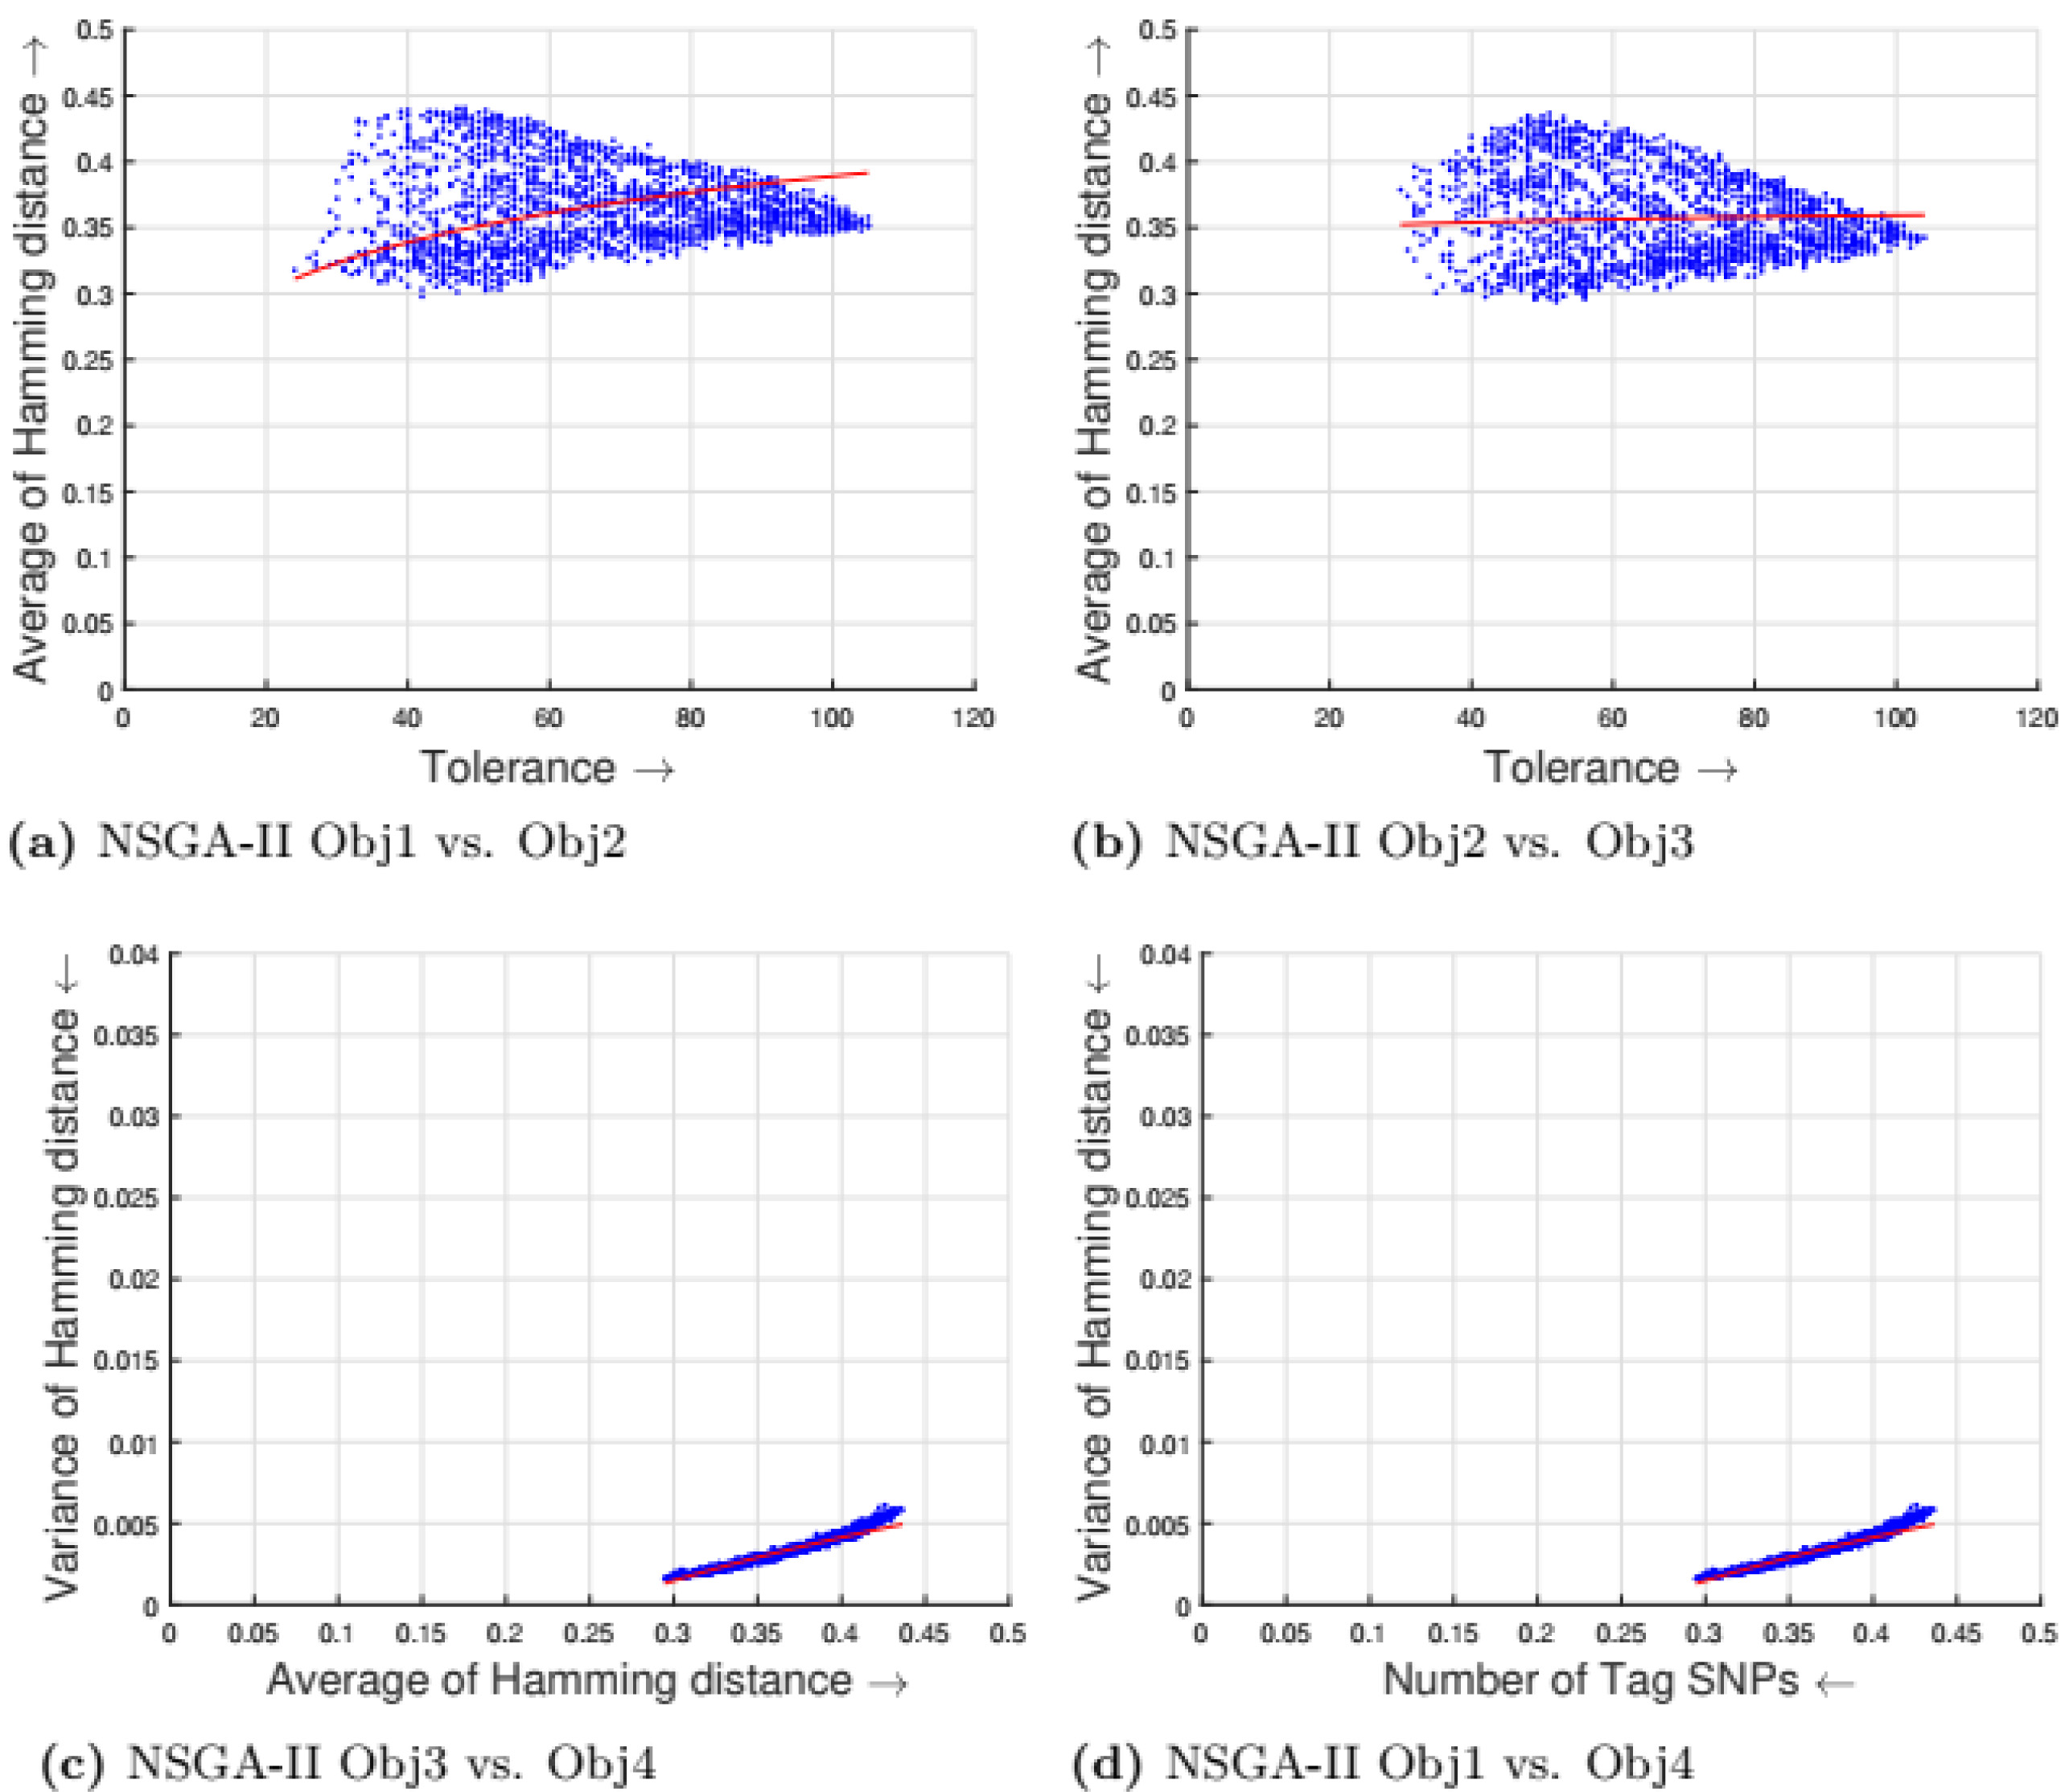
\includegraphics[width=\textwidth]{analisis_assets/moqa_2022/figures/moqa_fig_nsga2_random.jpeg}
        \caption{NSGA-II (RI)}
    \end{subfigure}
    \hfill
    \begin{subfigure}[b]{0.45\textwidth}
        \centering
        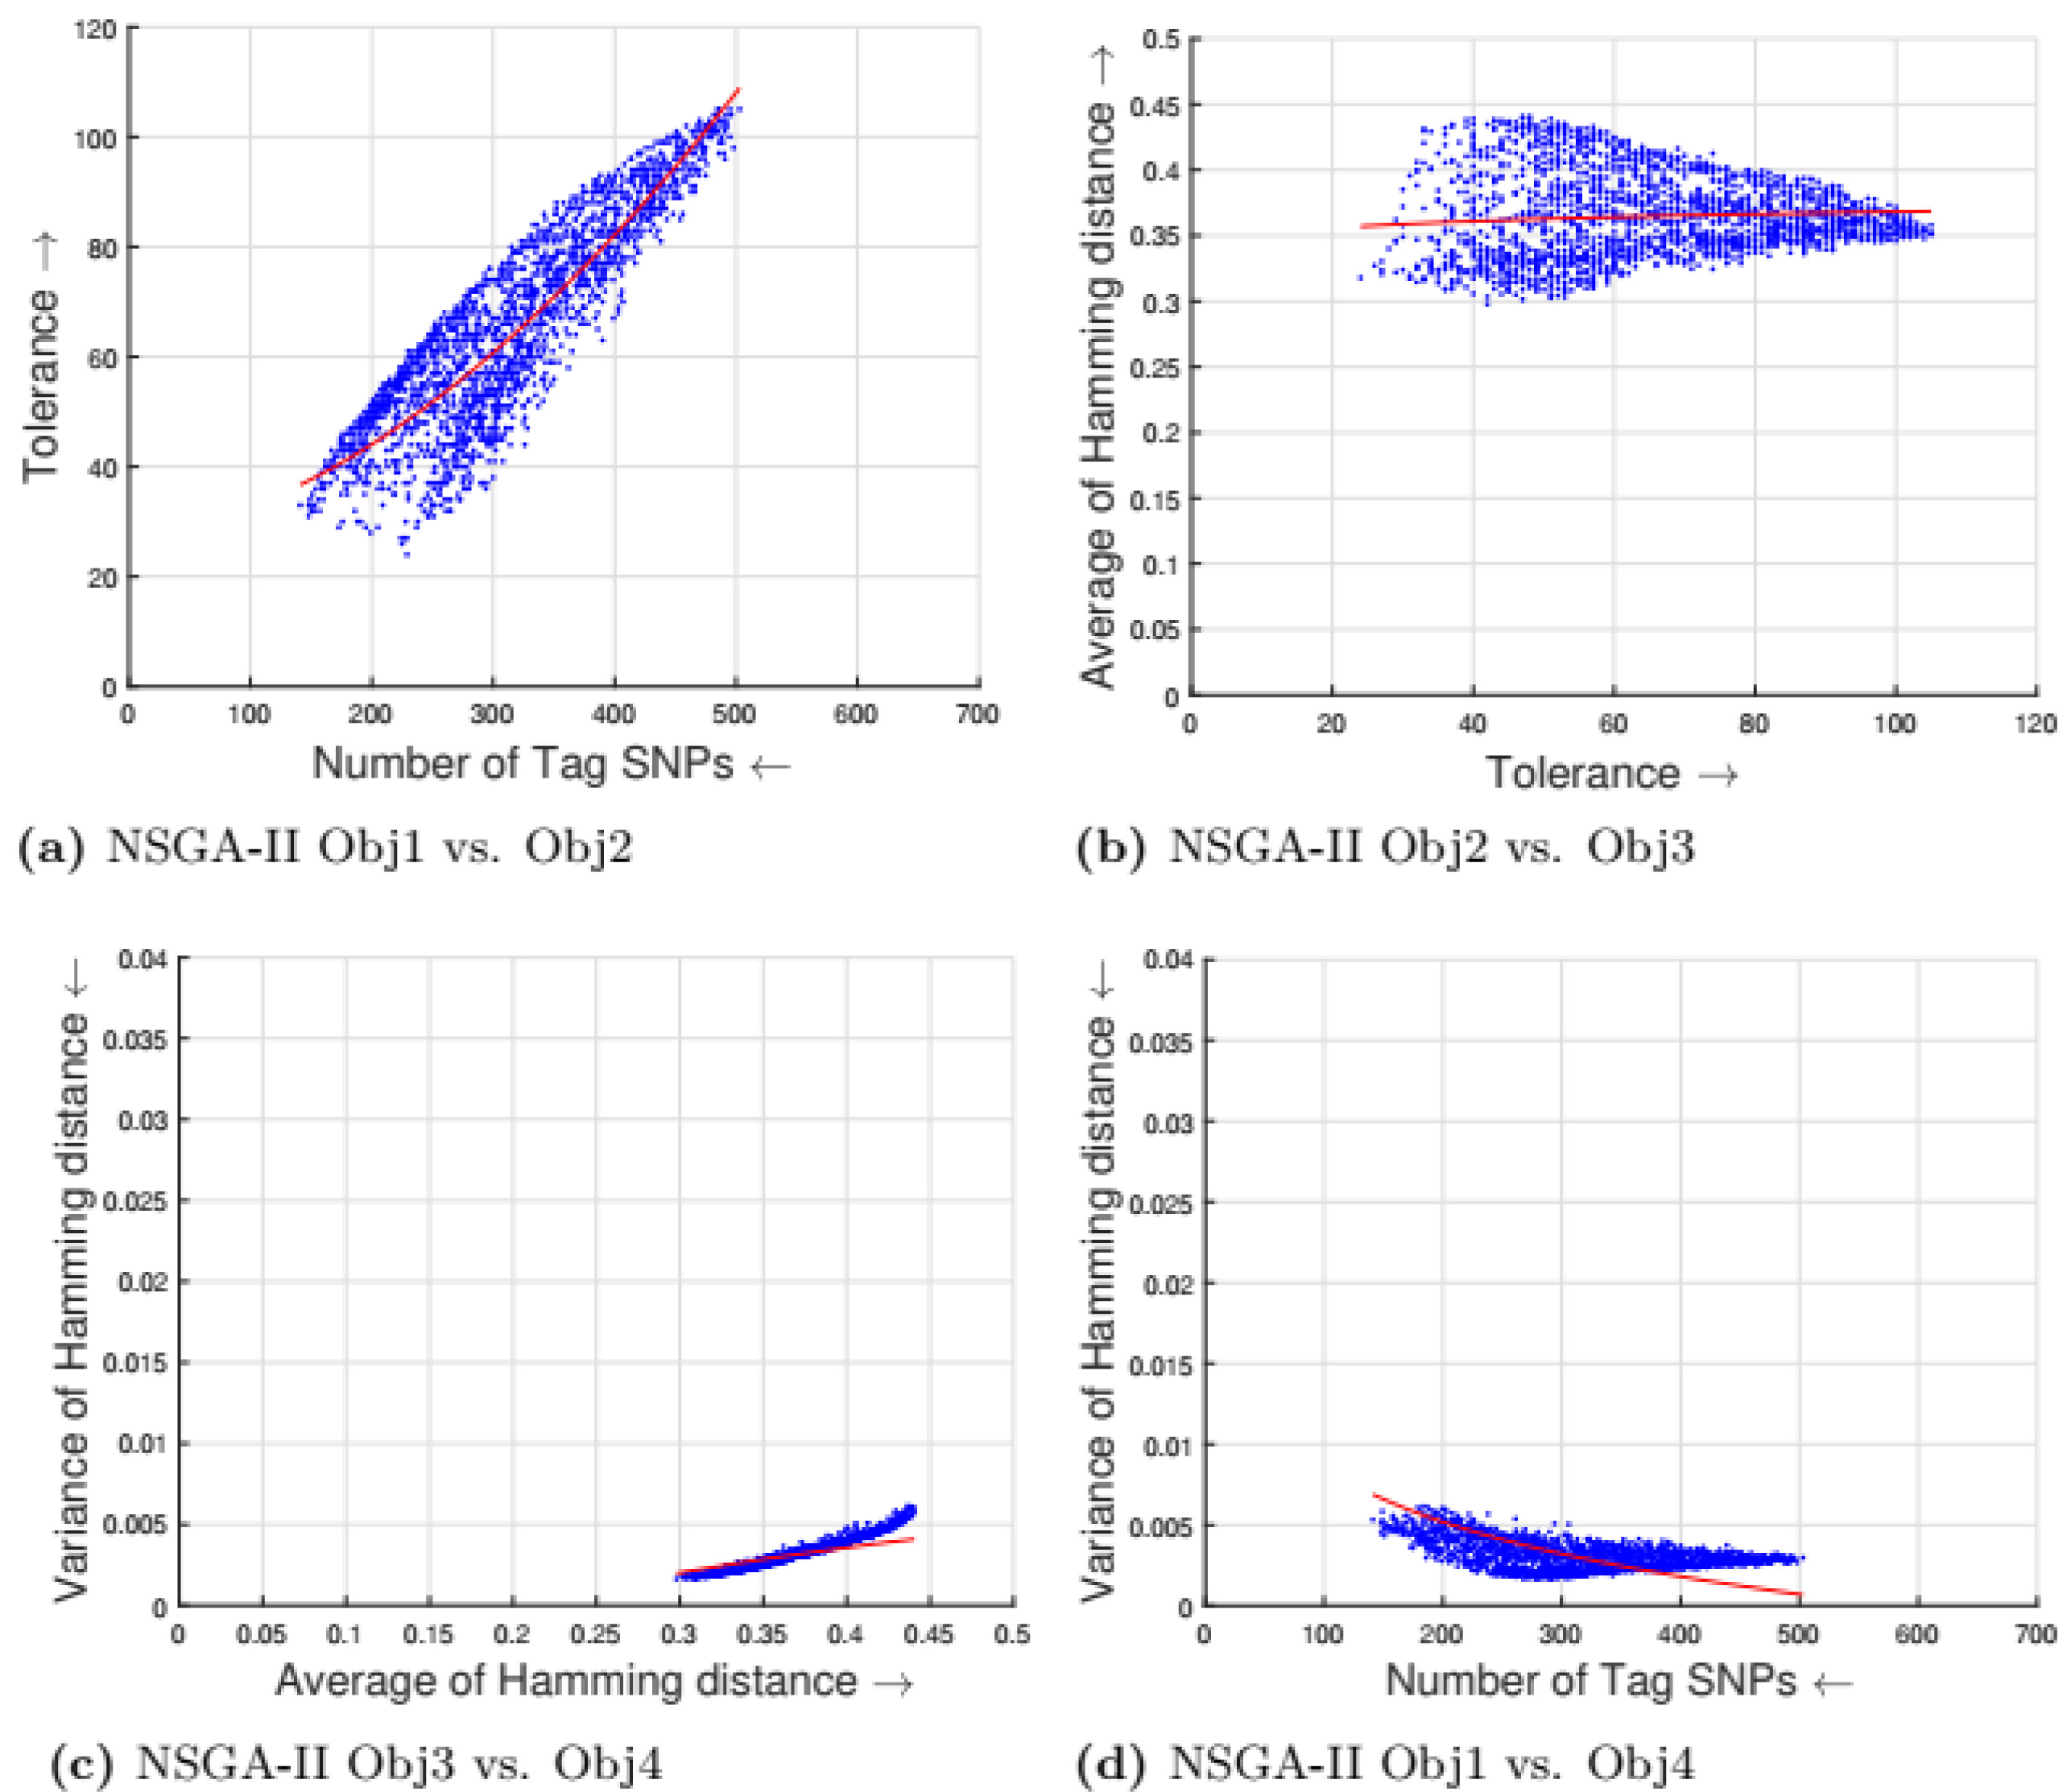
\includegraphics[width=\textwidth]{analisis_assets/moqa_2022/figures/moqa_fig_nsga2_greedy.jpeg}
        \caption{NSGA-II (GI)}
    \end{subfigure}
    \vskip\baselineskip
    \begin{subfigure}[b]{0.45\textwidth}
        \centering
        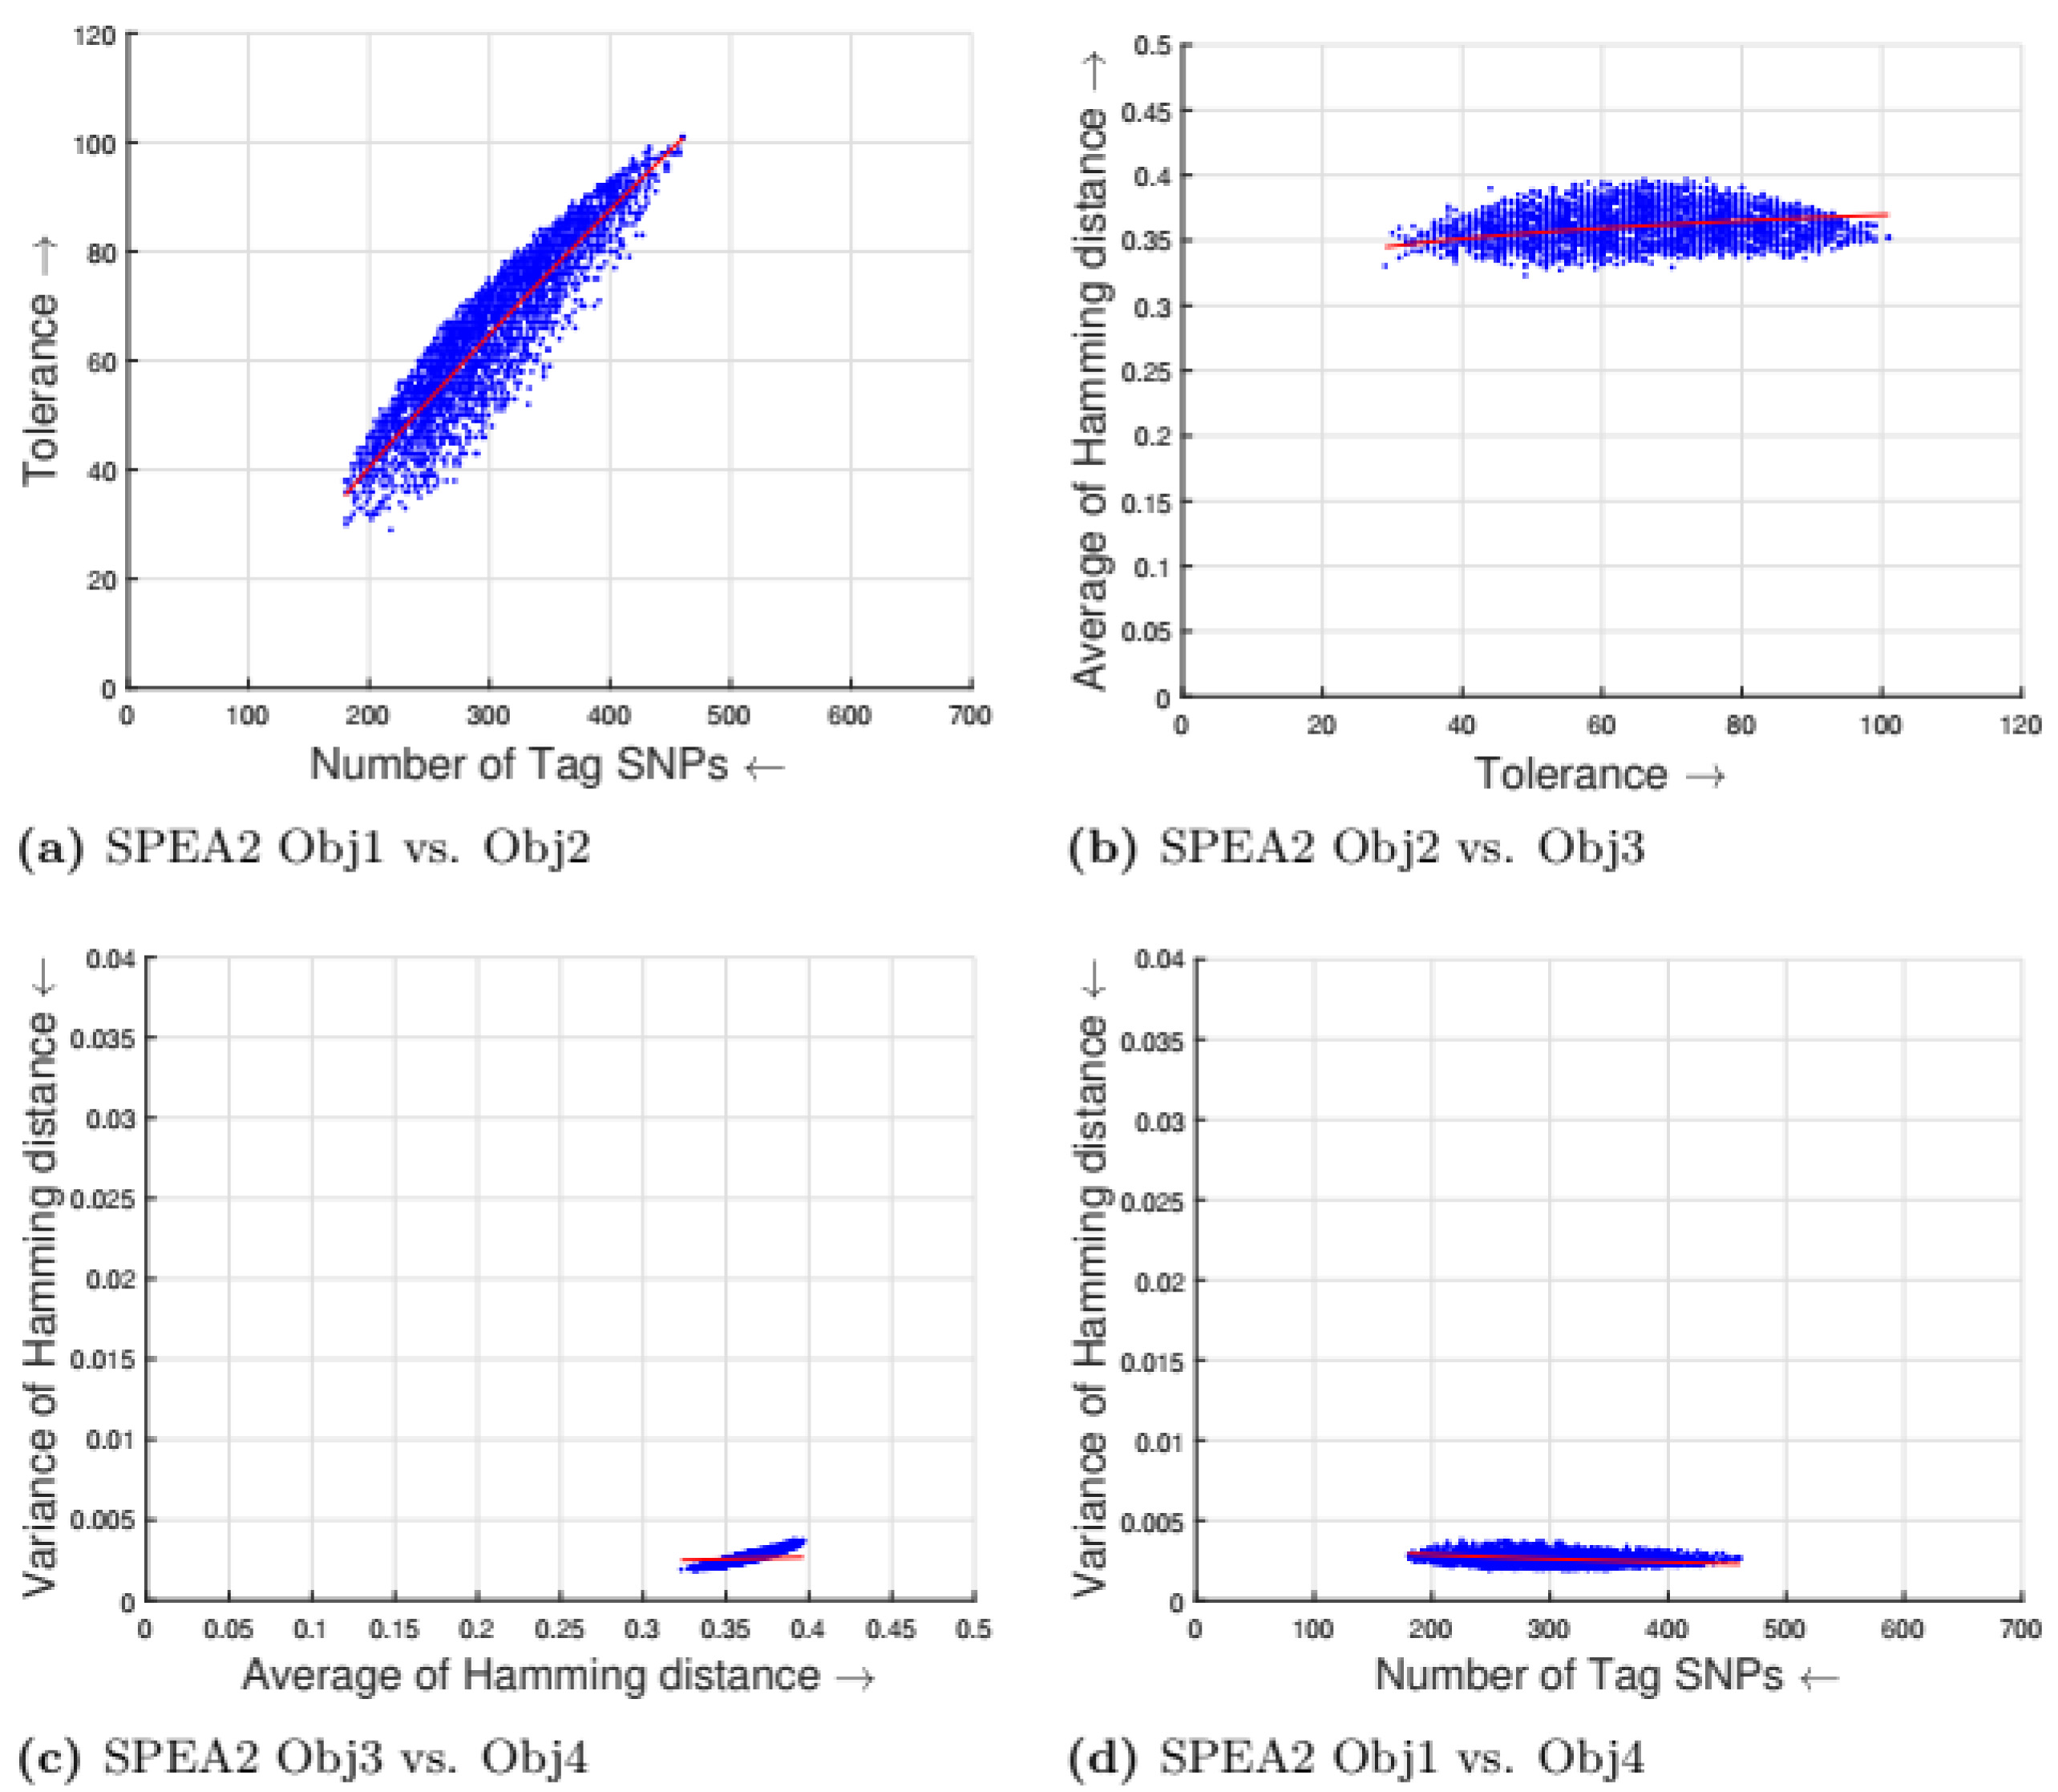
\includegraphics[width=\textwidth]{analisis_assets/moqa_2022/figures/moqa_fig_spea2_random.jpeg}
        \caption{SPEA2 (RI)}
    \end{subfigure}
    \hfill
    \begin{subfigure}[b]{0.45\textwidth}
        \centering
        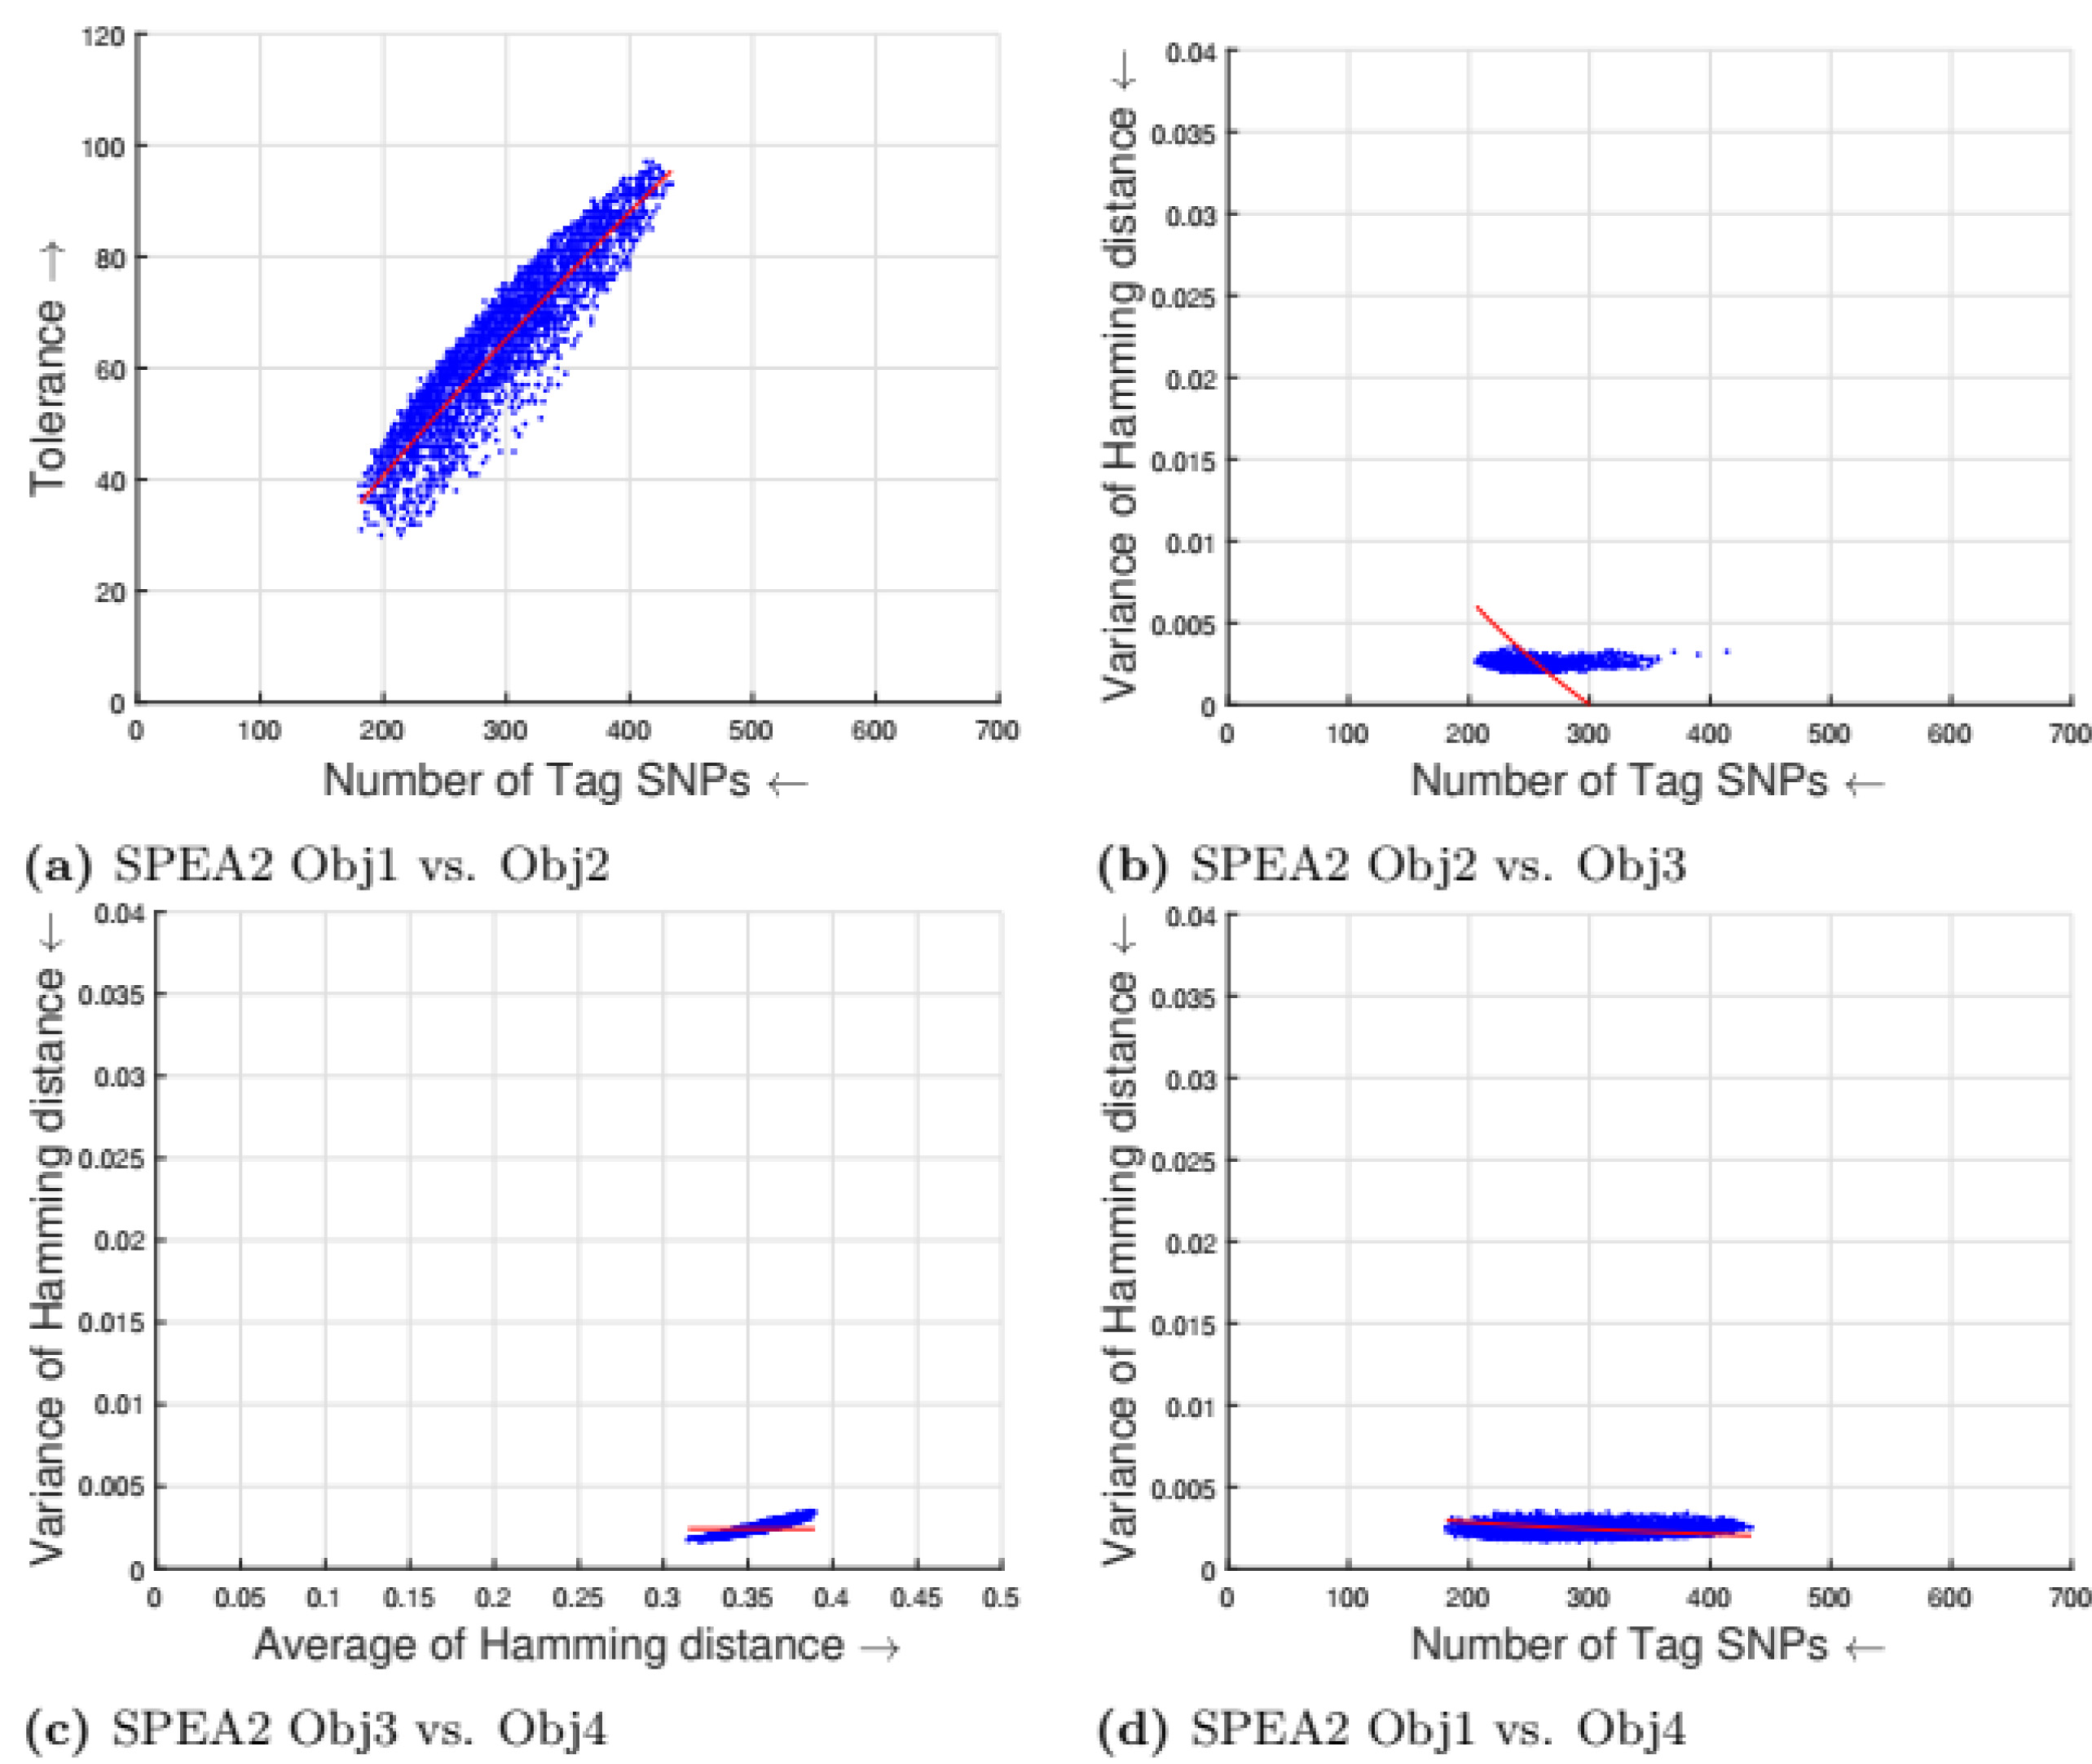
\includegraphics[width=\textwidth]{analisis_assets/moqa_2022/figures/moqa_fig_spea2_greedy.jpeg}
        \caption{SPEA2 (GI)}
    \end{subfigure}
    \caption{Comparativa de Frentes de Pareto: NSGA-II y SPEA2 (Moqa 2022).}
\end{figure}

\begin{figure}[H]
    \centering
    \begin{subfigure}[b]{0.45\textwidth}
        \centering
        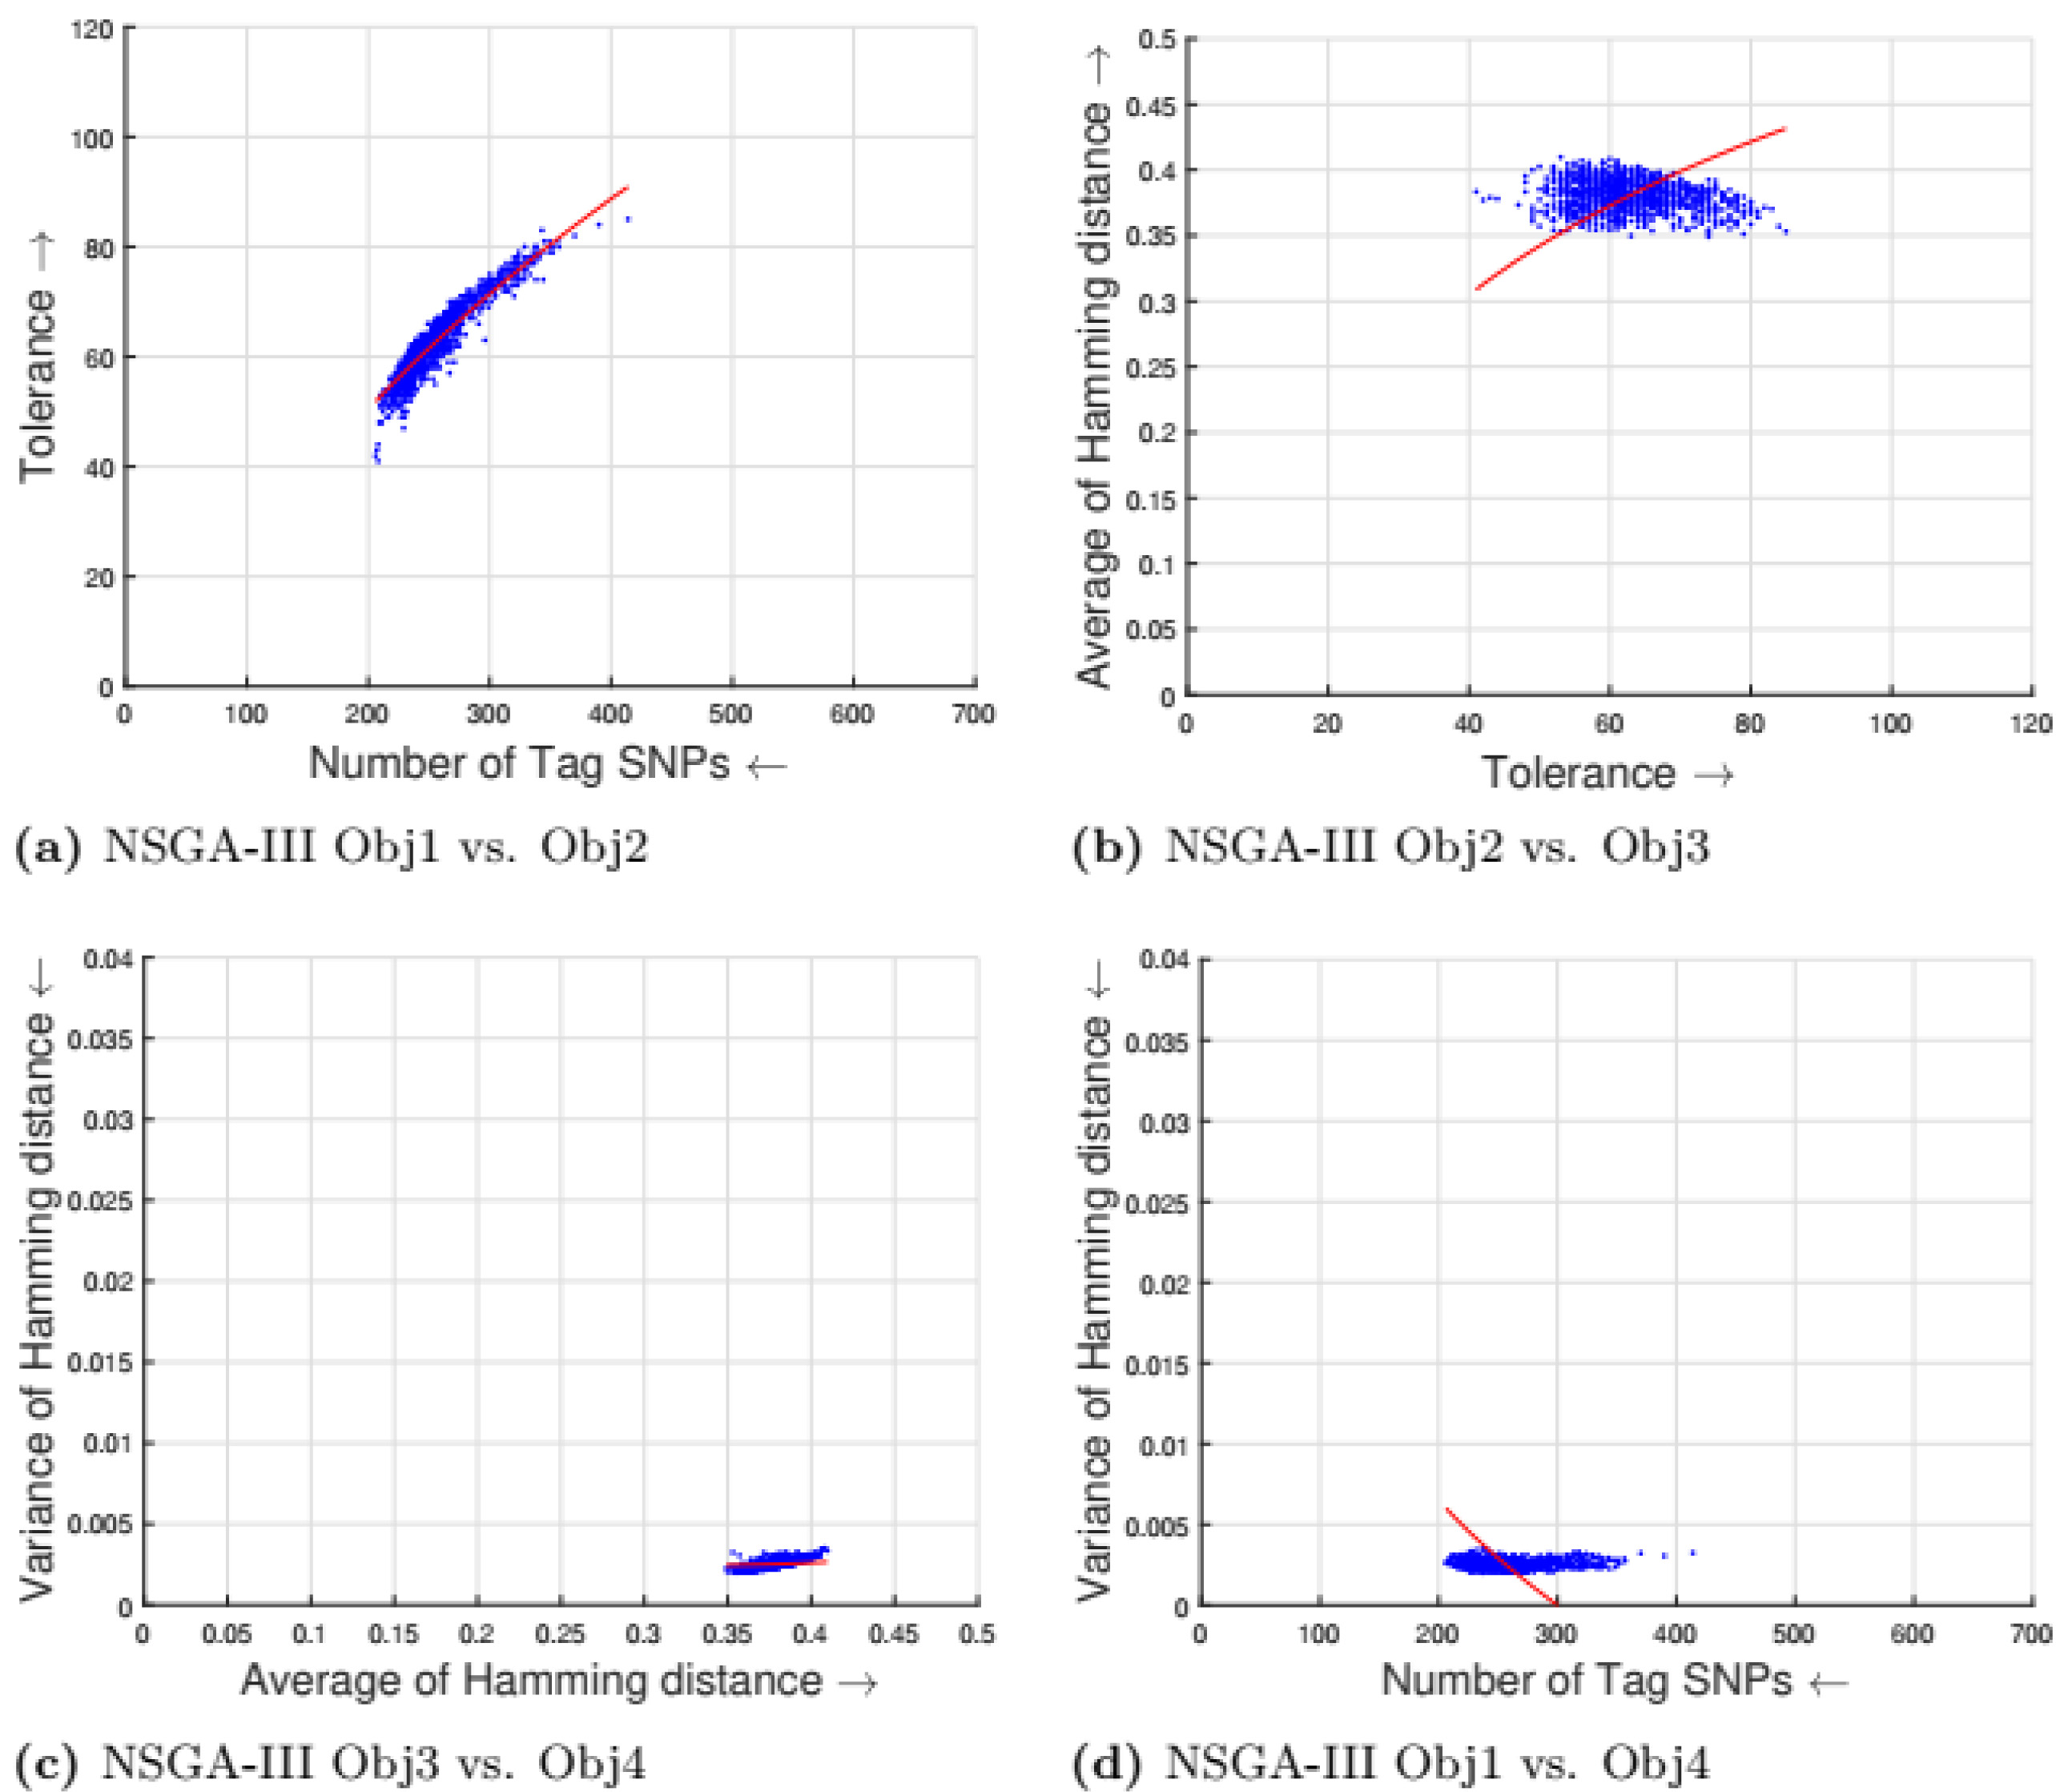
\includegraphics[width=\textwidth]{analisis_assets/moqa_2022/figures/moqa_fig_nsga3_random.jpeg}
        \caption{NSGA-III (RI)}
    \end{subfigure}
    \hfill
    \begin{subfigure}[b]{0.45\textwidth}
        \centering
        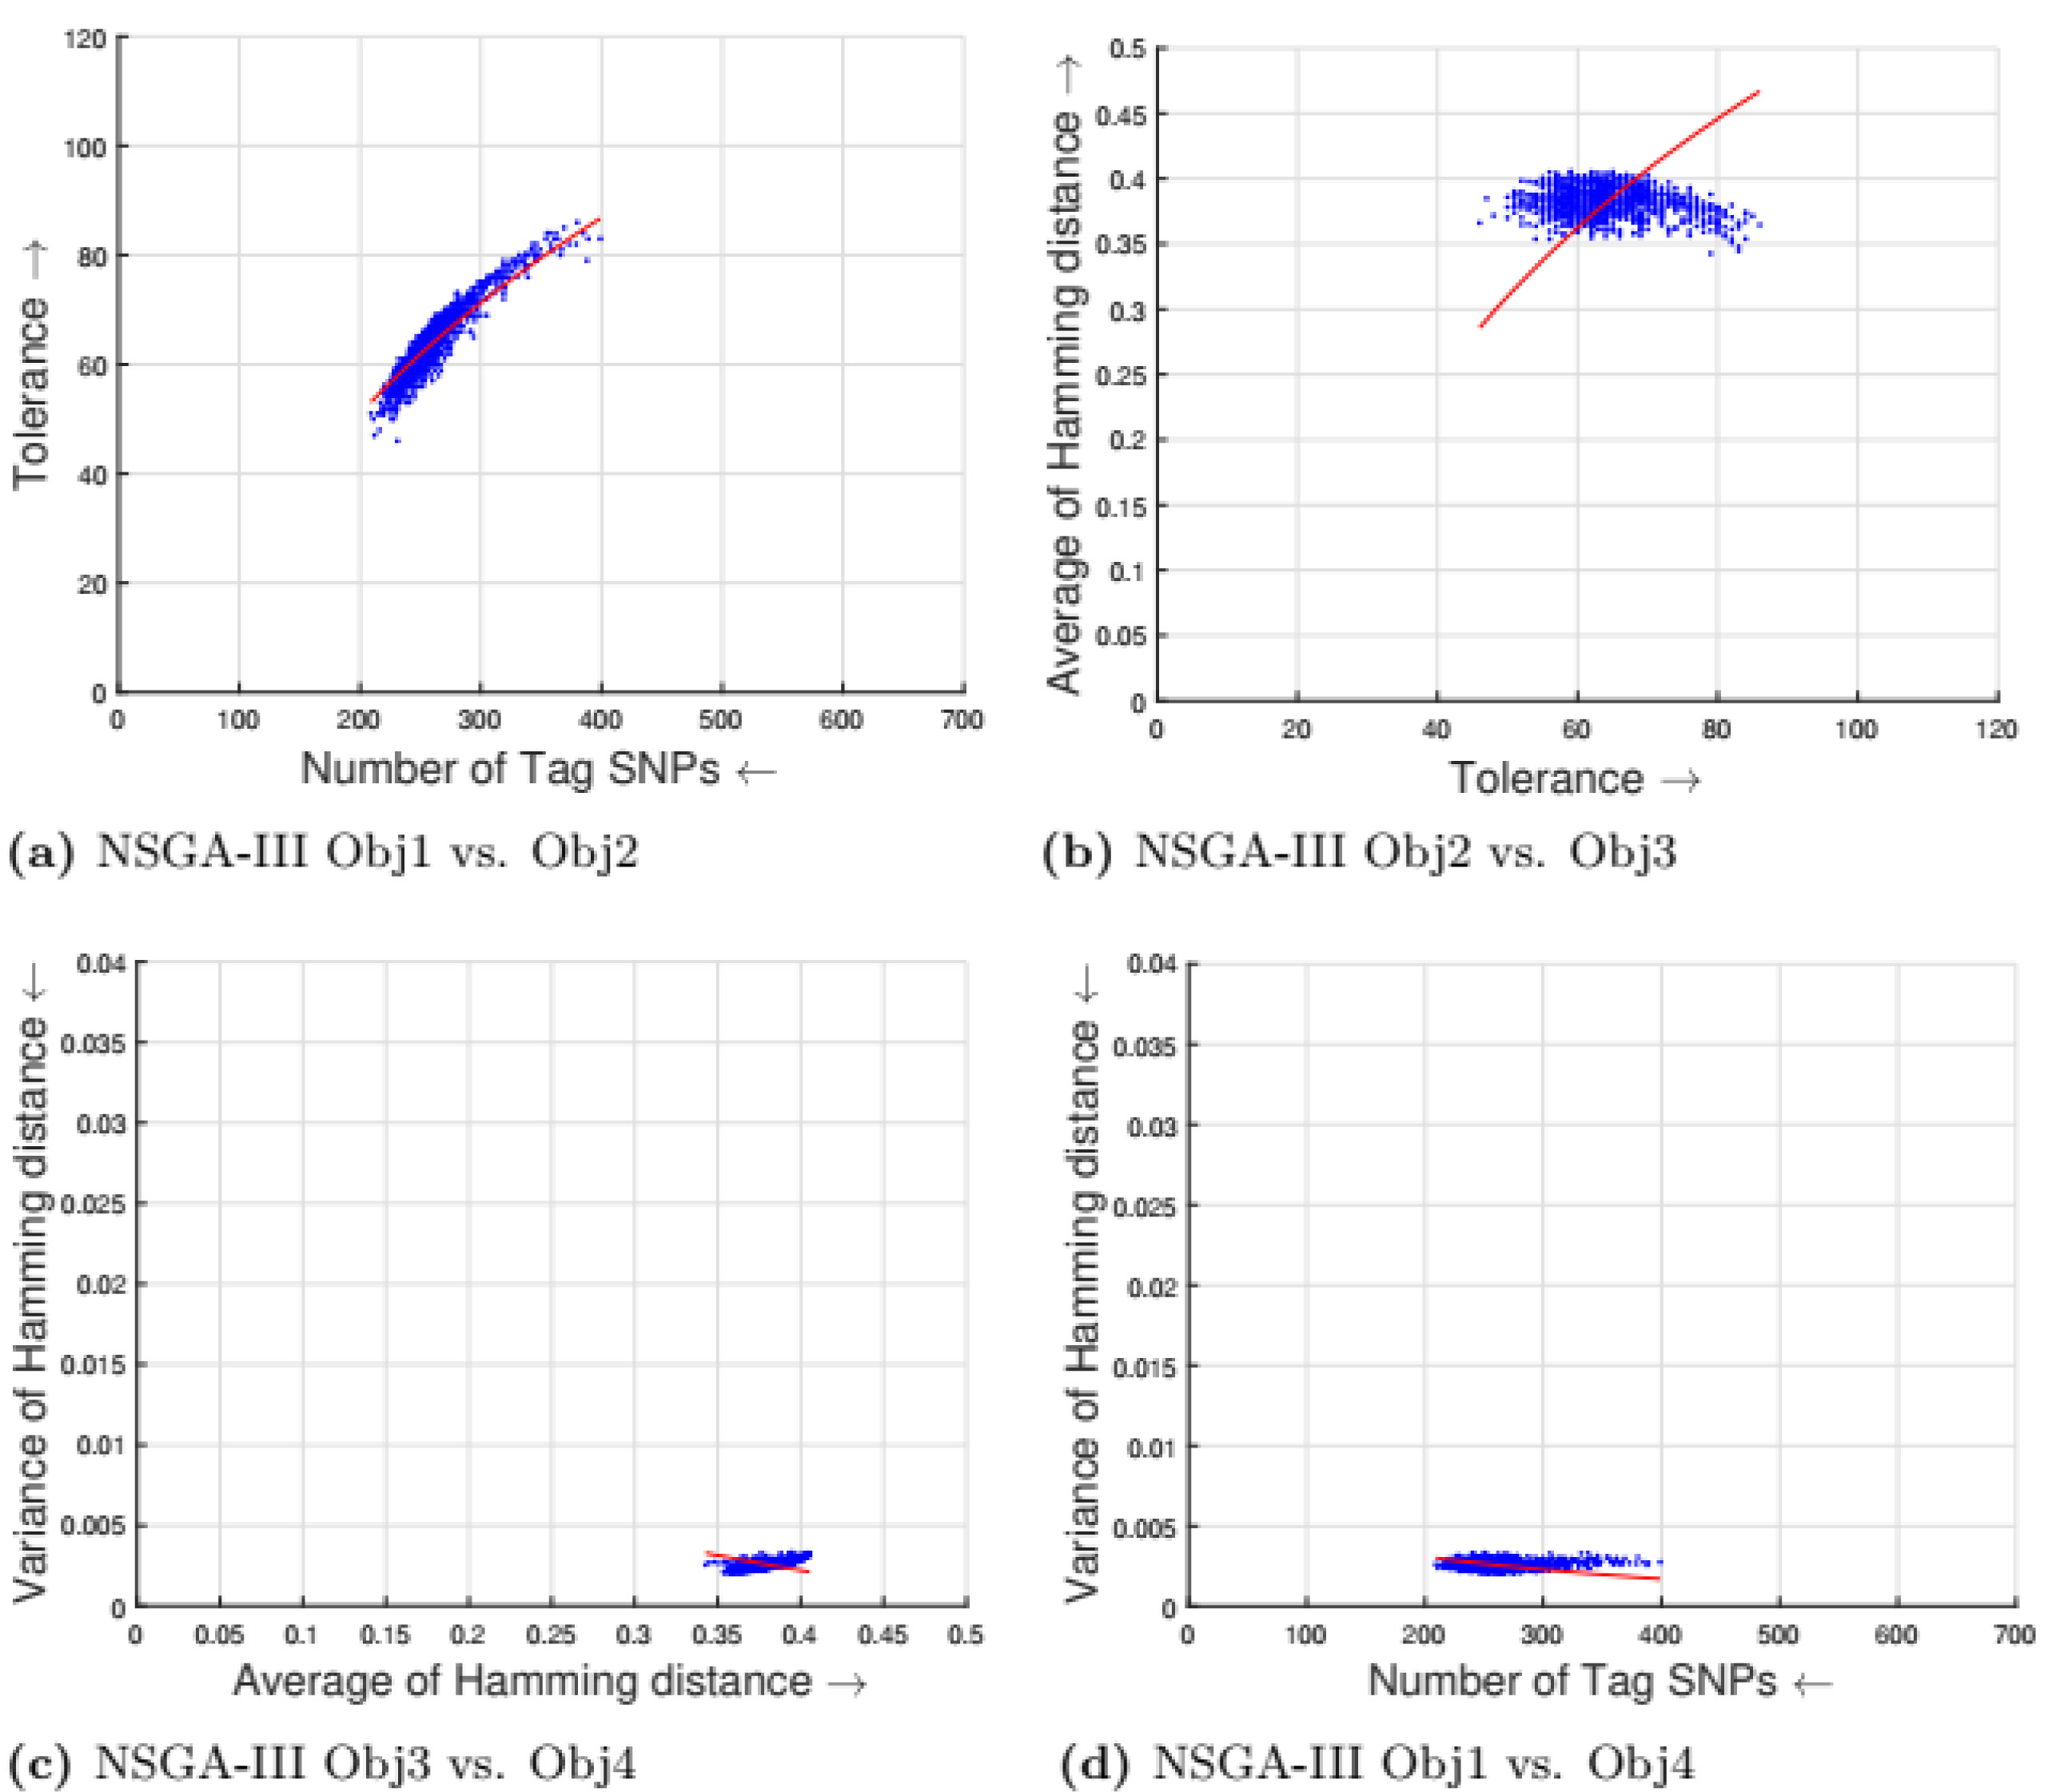
\includegraphics[width=\textwidth]{analisis_assets/moqa_2022/figures/moqa_fig_nsga3_greedy.jpeg}
        \caption{NSGA-III (GI)}
    \end{subfigure}
    \vskip\baselineskip
    \begin{subfigure}[b]{0.45\textwidth}
        \centering
        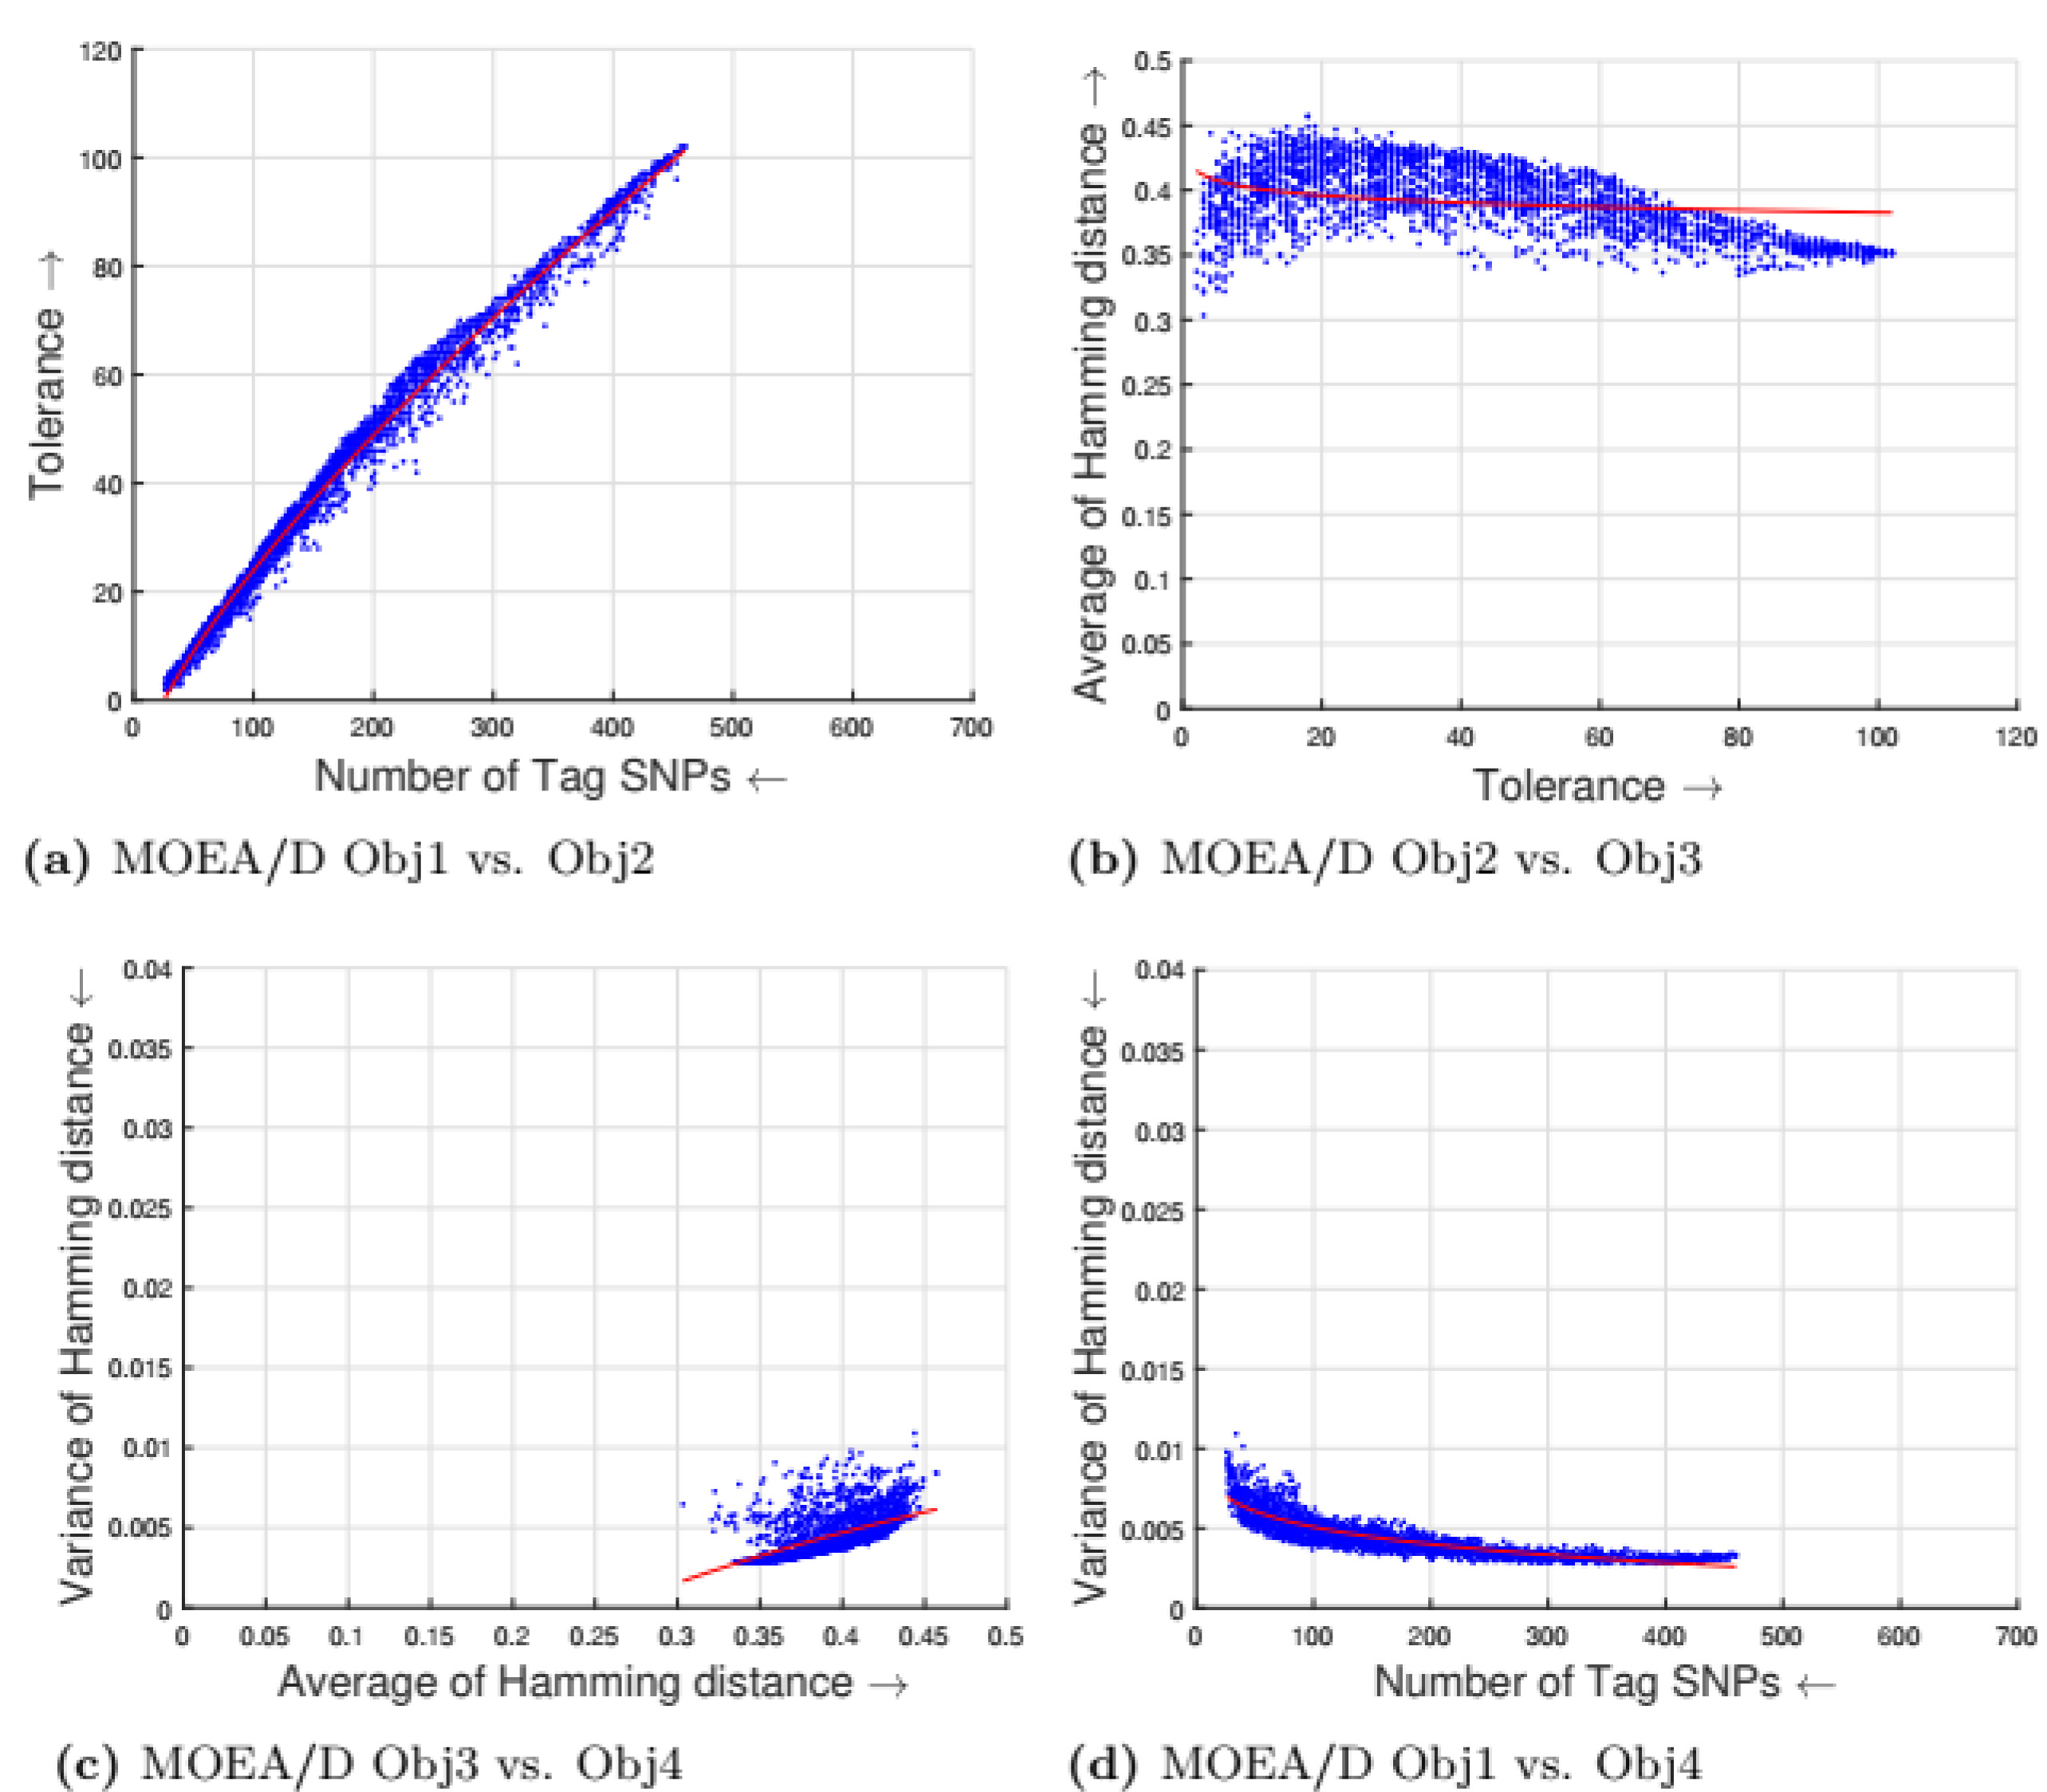
\includegraphics[width=\textwidth]{analisis_assets/moqa_2022/figures/moqa_fig_moead_random.jpeg}
        \caption{MOEA/D (RI)}
    \end{subfigure}
    \hfill
    \begin{subfigure}[b]{0.45\textwidth}
        \centering
        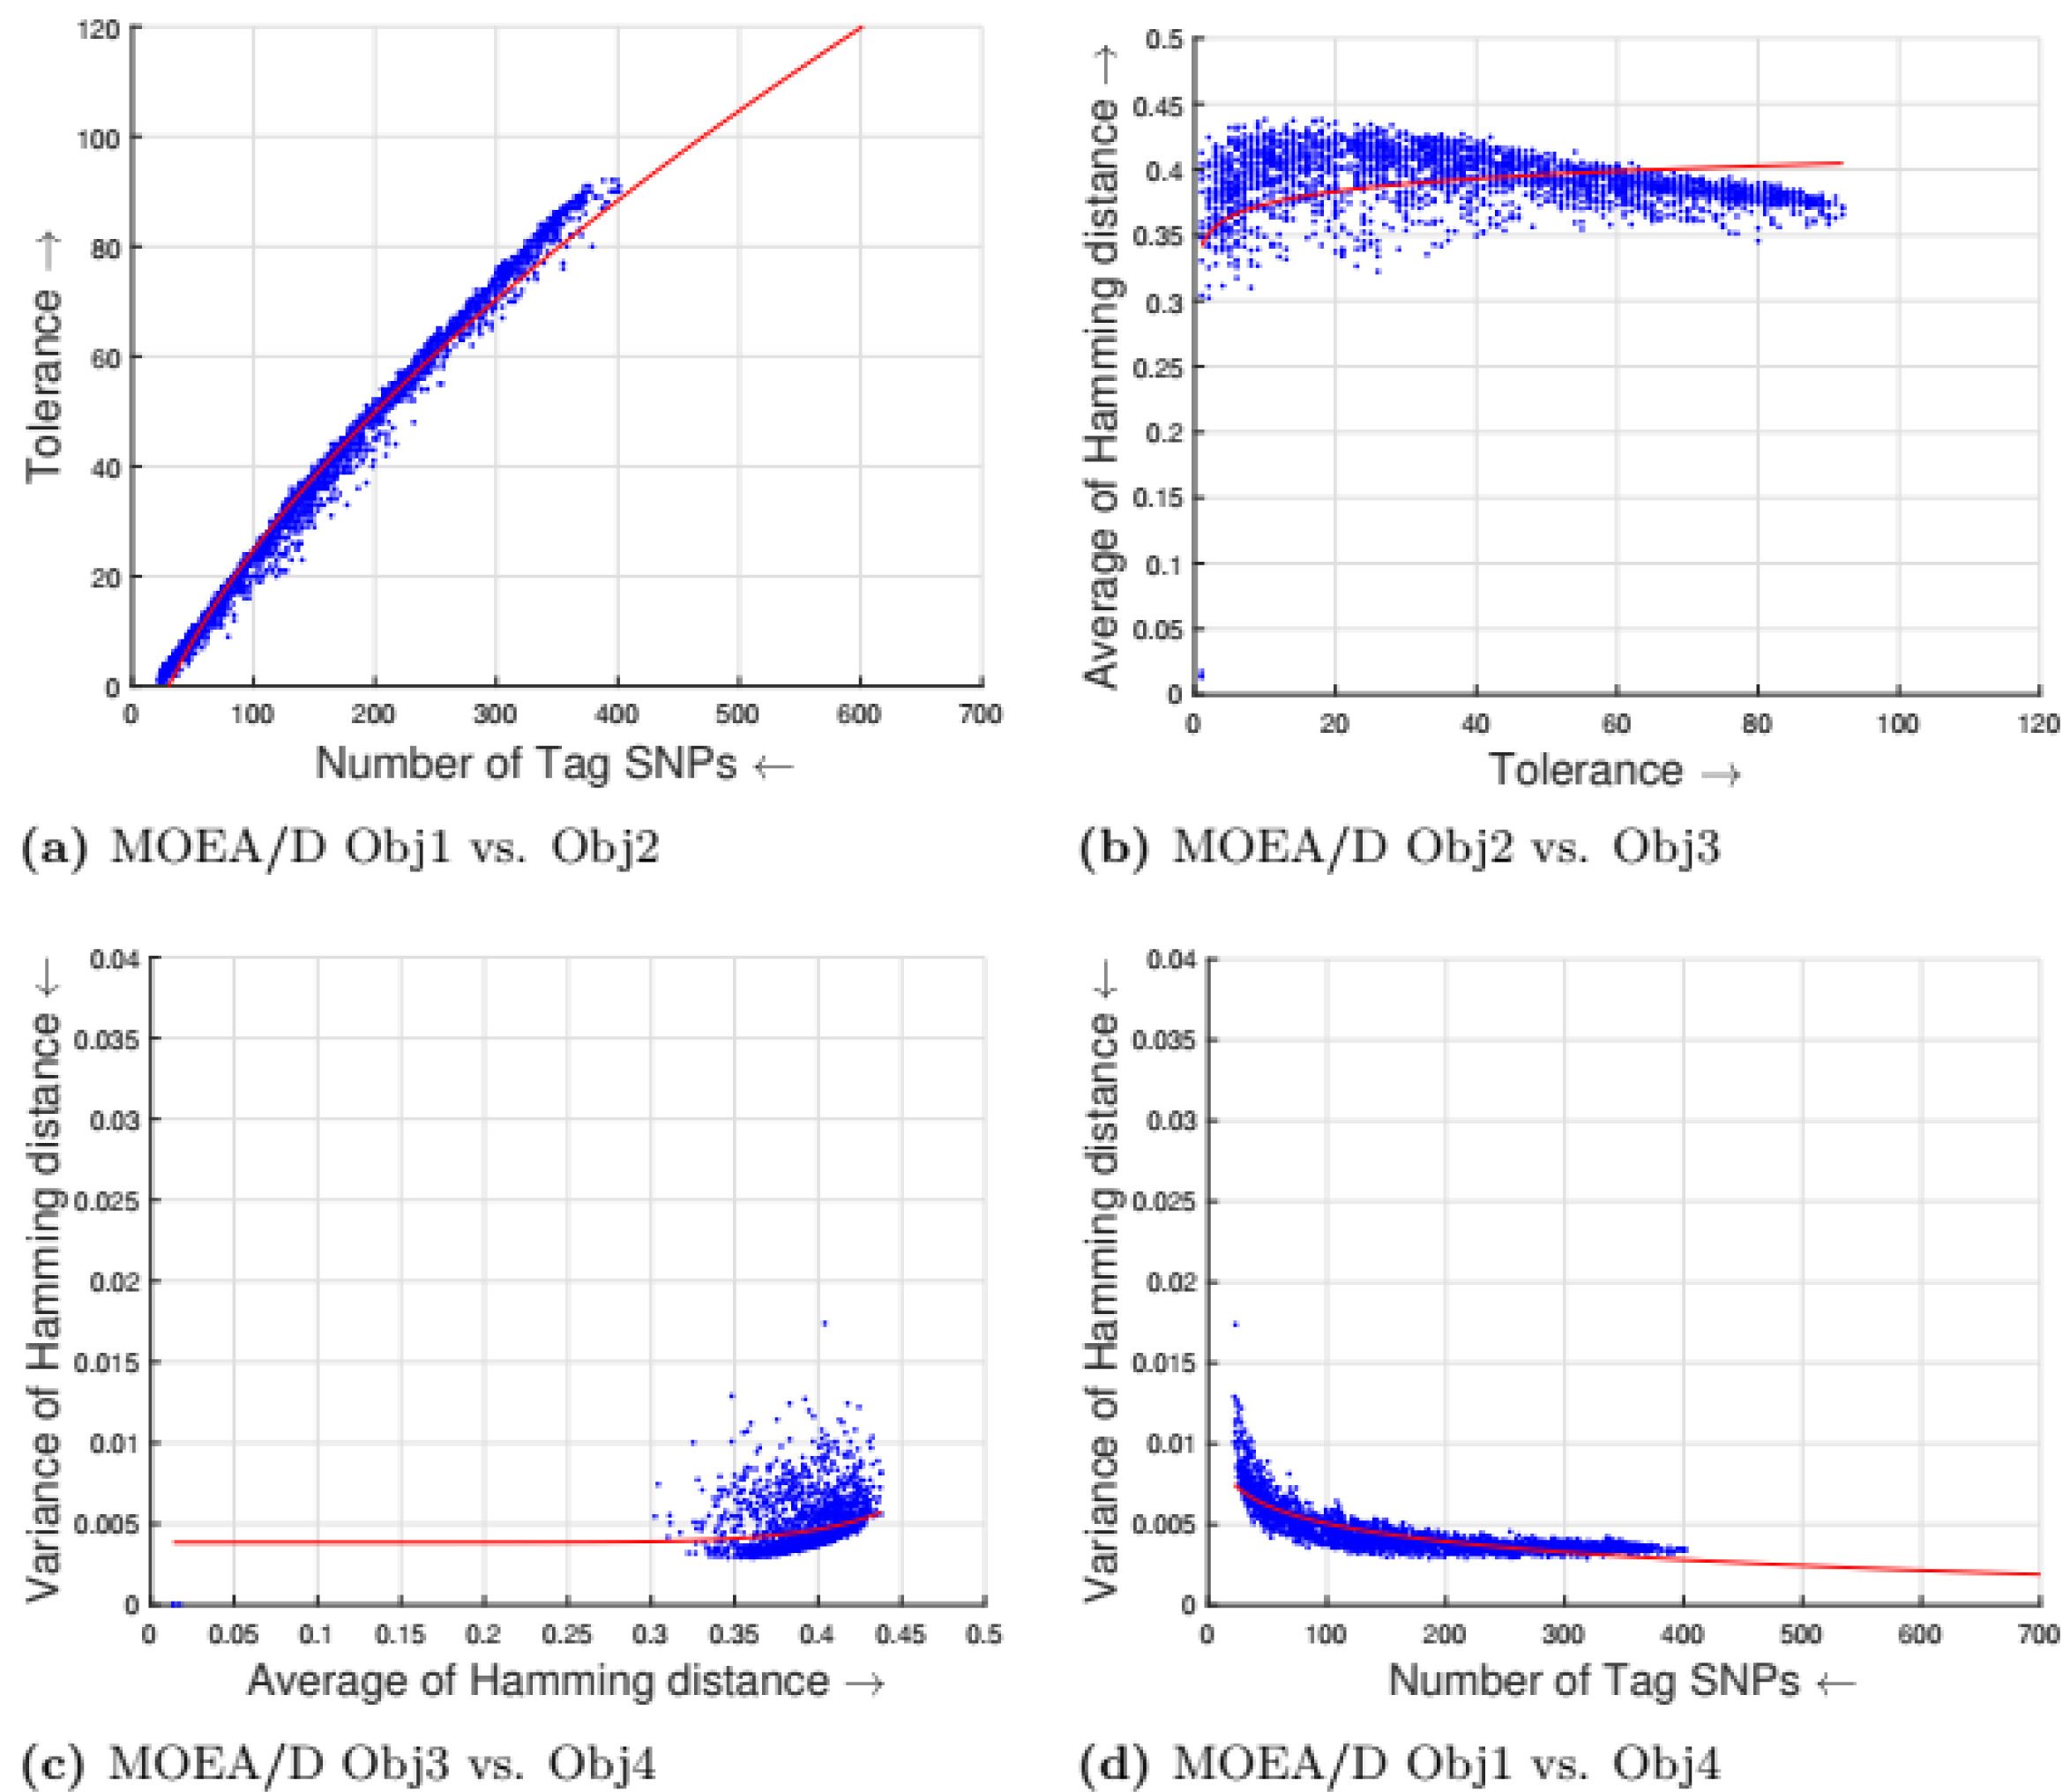
\includegraphics[width=\textwidth]{analisis_assets/moqa_2022/figures/moqa_fig_moead_greedy.jpeg}
        \caption{MOEA/D (GI)}
    \end{subfigure}
    \caption{Comparativa de Frentes de Pareto: NSGA-III y MOEA/D (Moqa 2022).}
\end{figure}

\subsubsection{Convergencia progresiva}
\begin{figure}[H]
    \centering
    \begin{subfigure}[b]{0.48\textwidth}
        \centering
        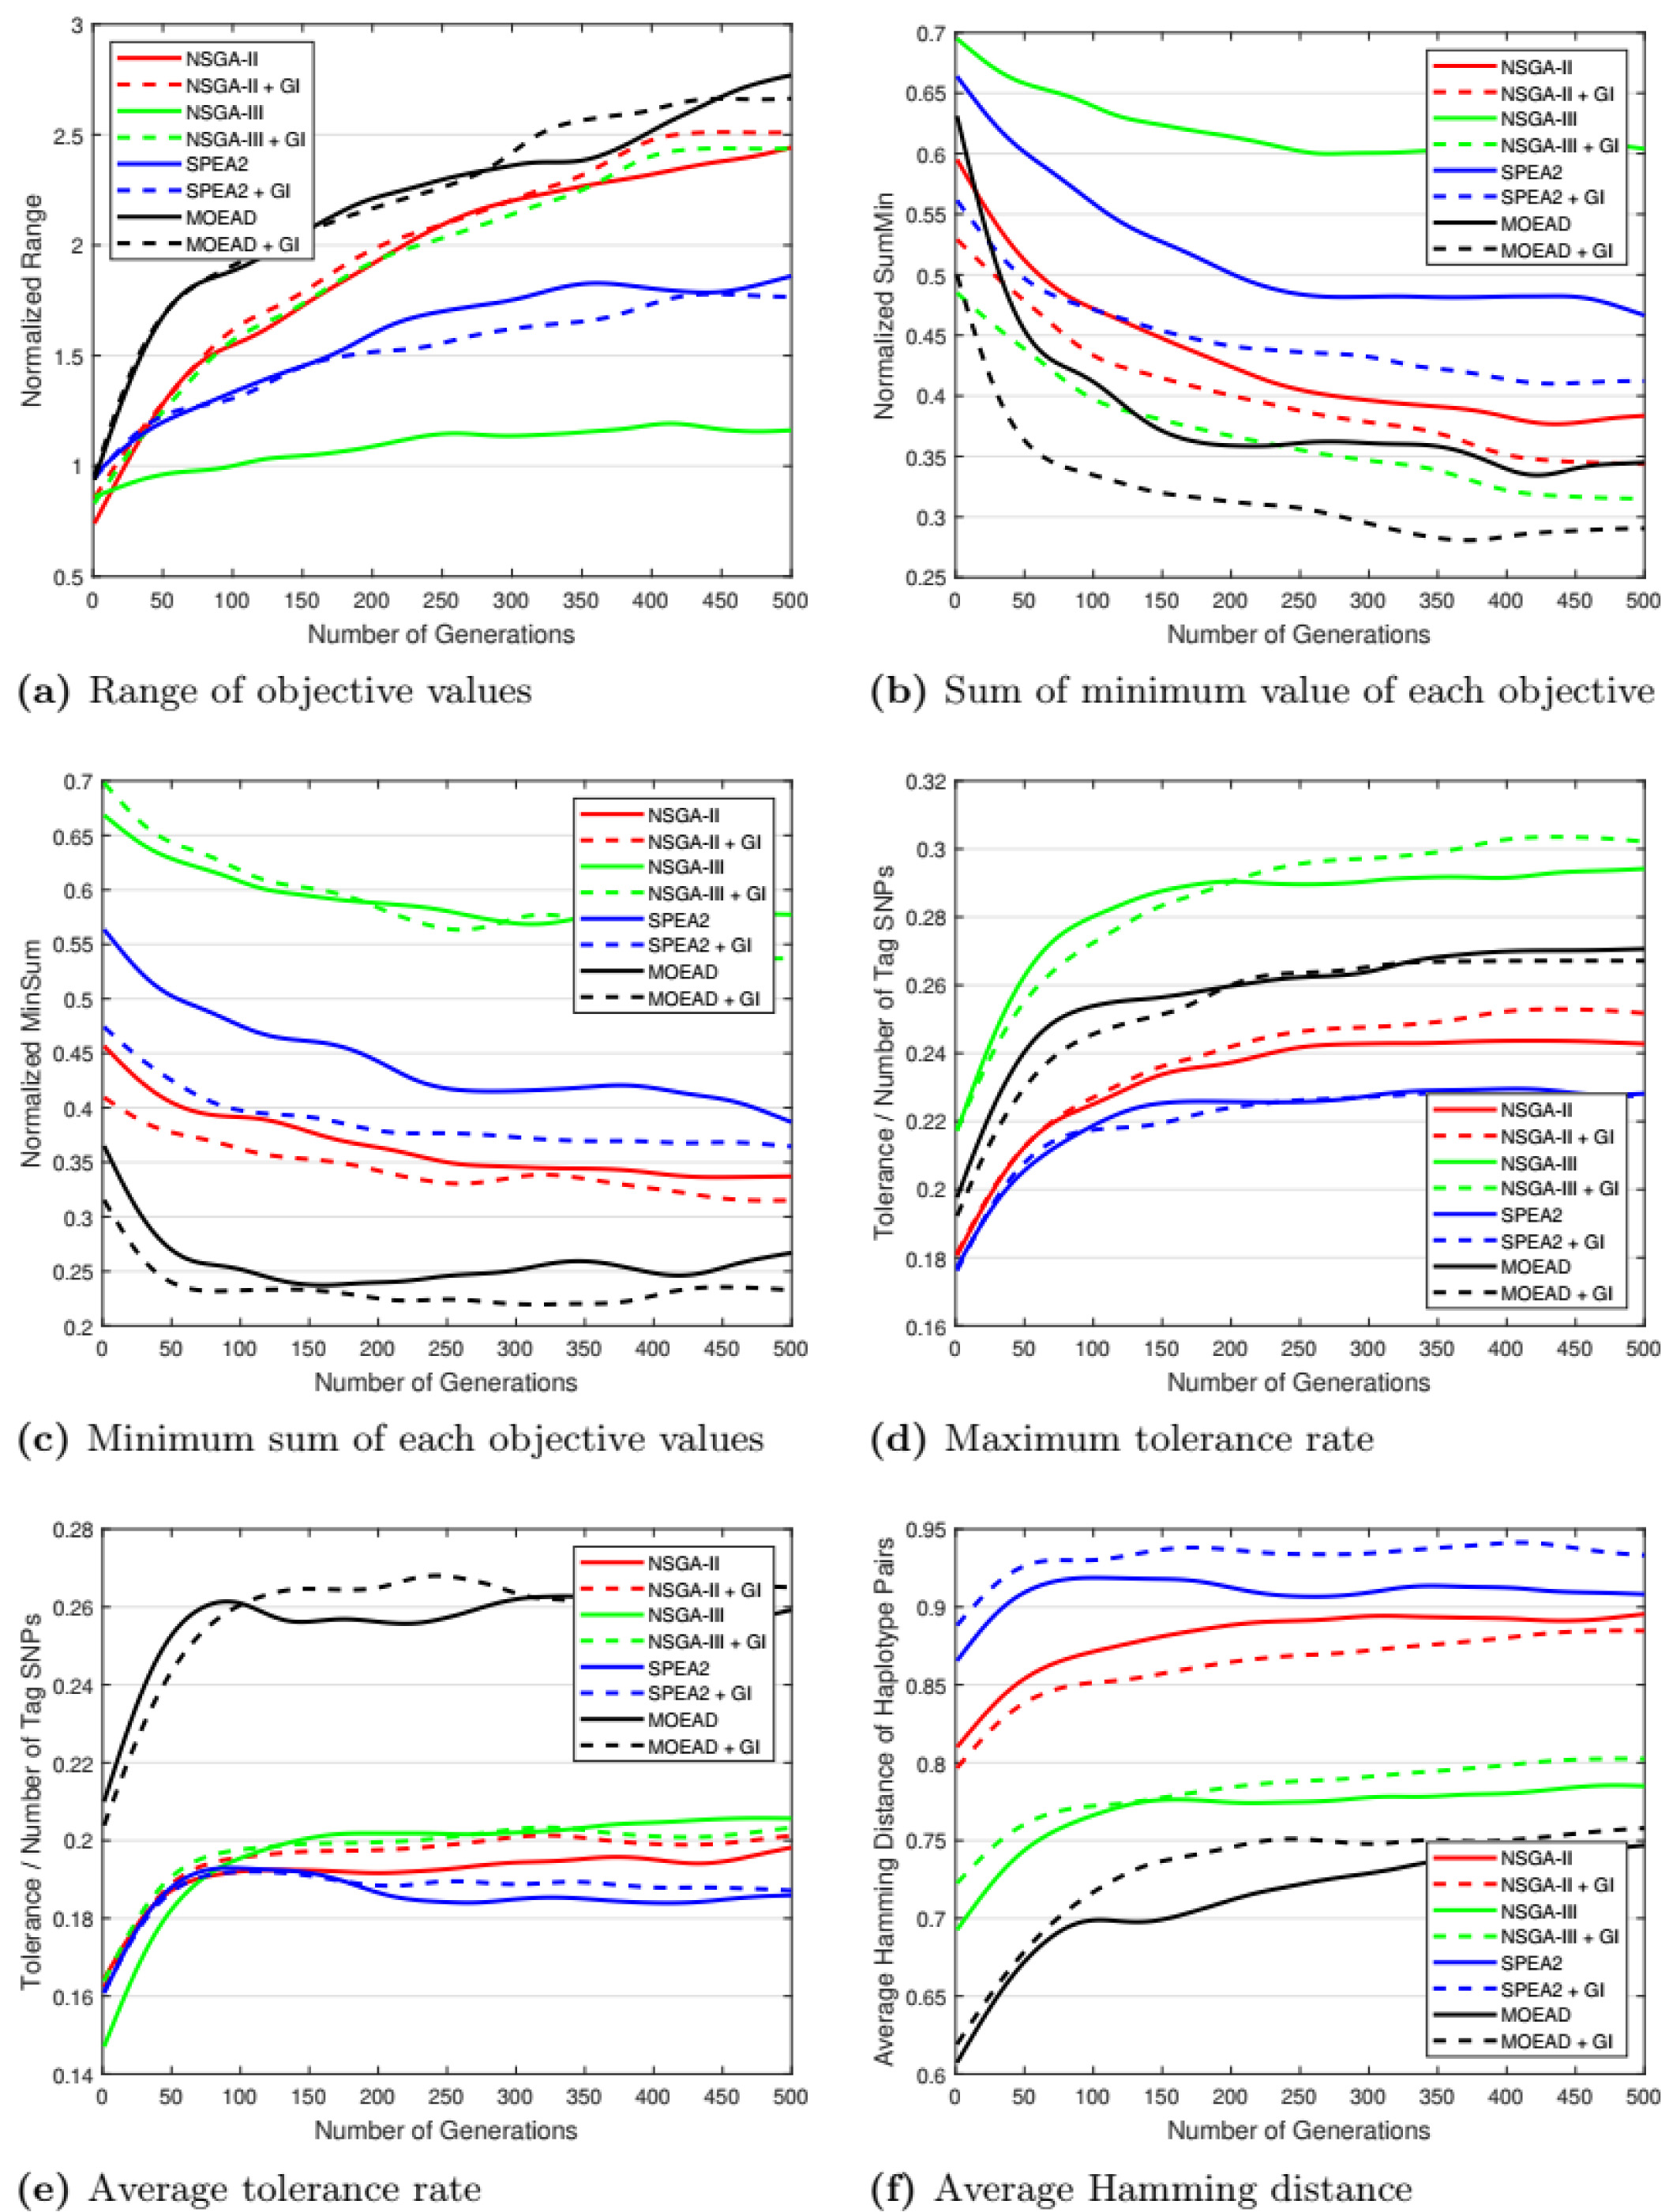
\includegraphics[width=\textwidth]{analisis_assets/moqa_2022/figures/moqa_fig_convergencia_1.jpeg}
        \caption{Evolución por generación de seis métricas de rendimiento en el experimento base (500 generaciones, población = 200). Se ilustra el impacto de la inicialización heurística (GI, líneas discontinuas) frente a la aleatoria (RI, líneas continuas).}
    \end{subfigure}
    \hfill
    \begin{subfigure}[b]{0.48\textwidth}
        \centering
        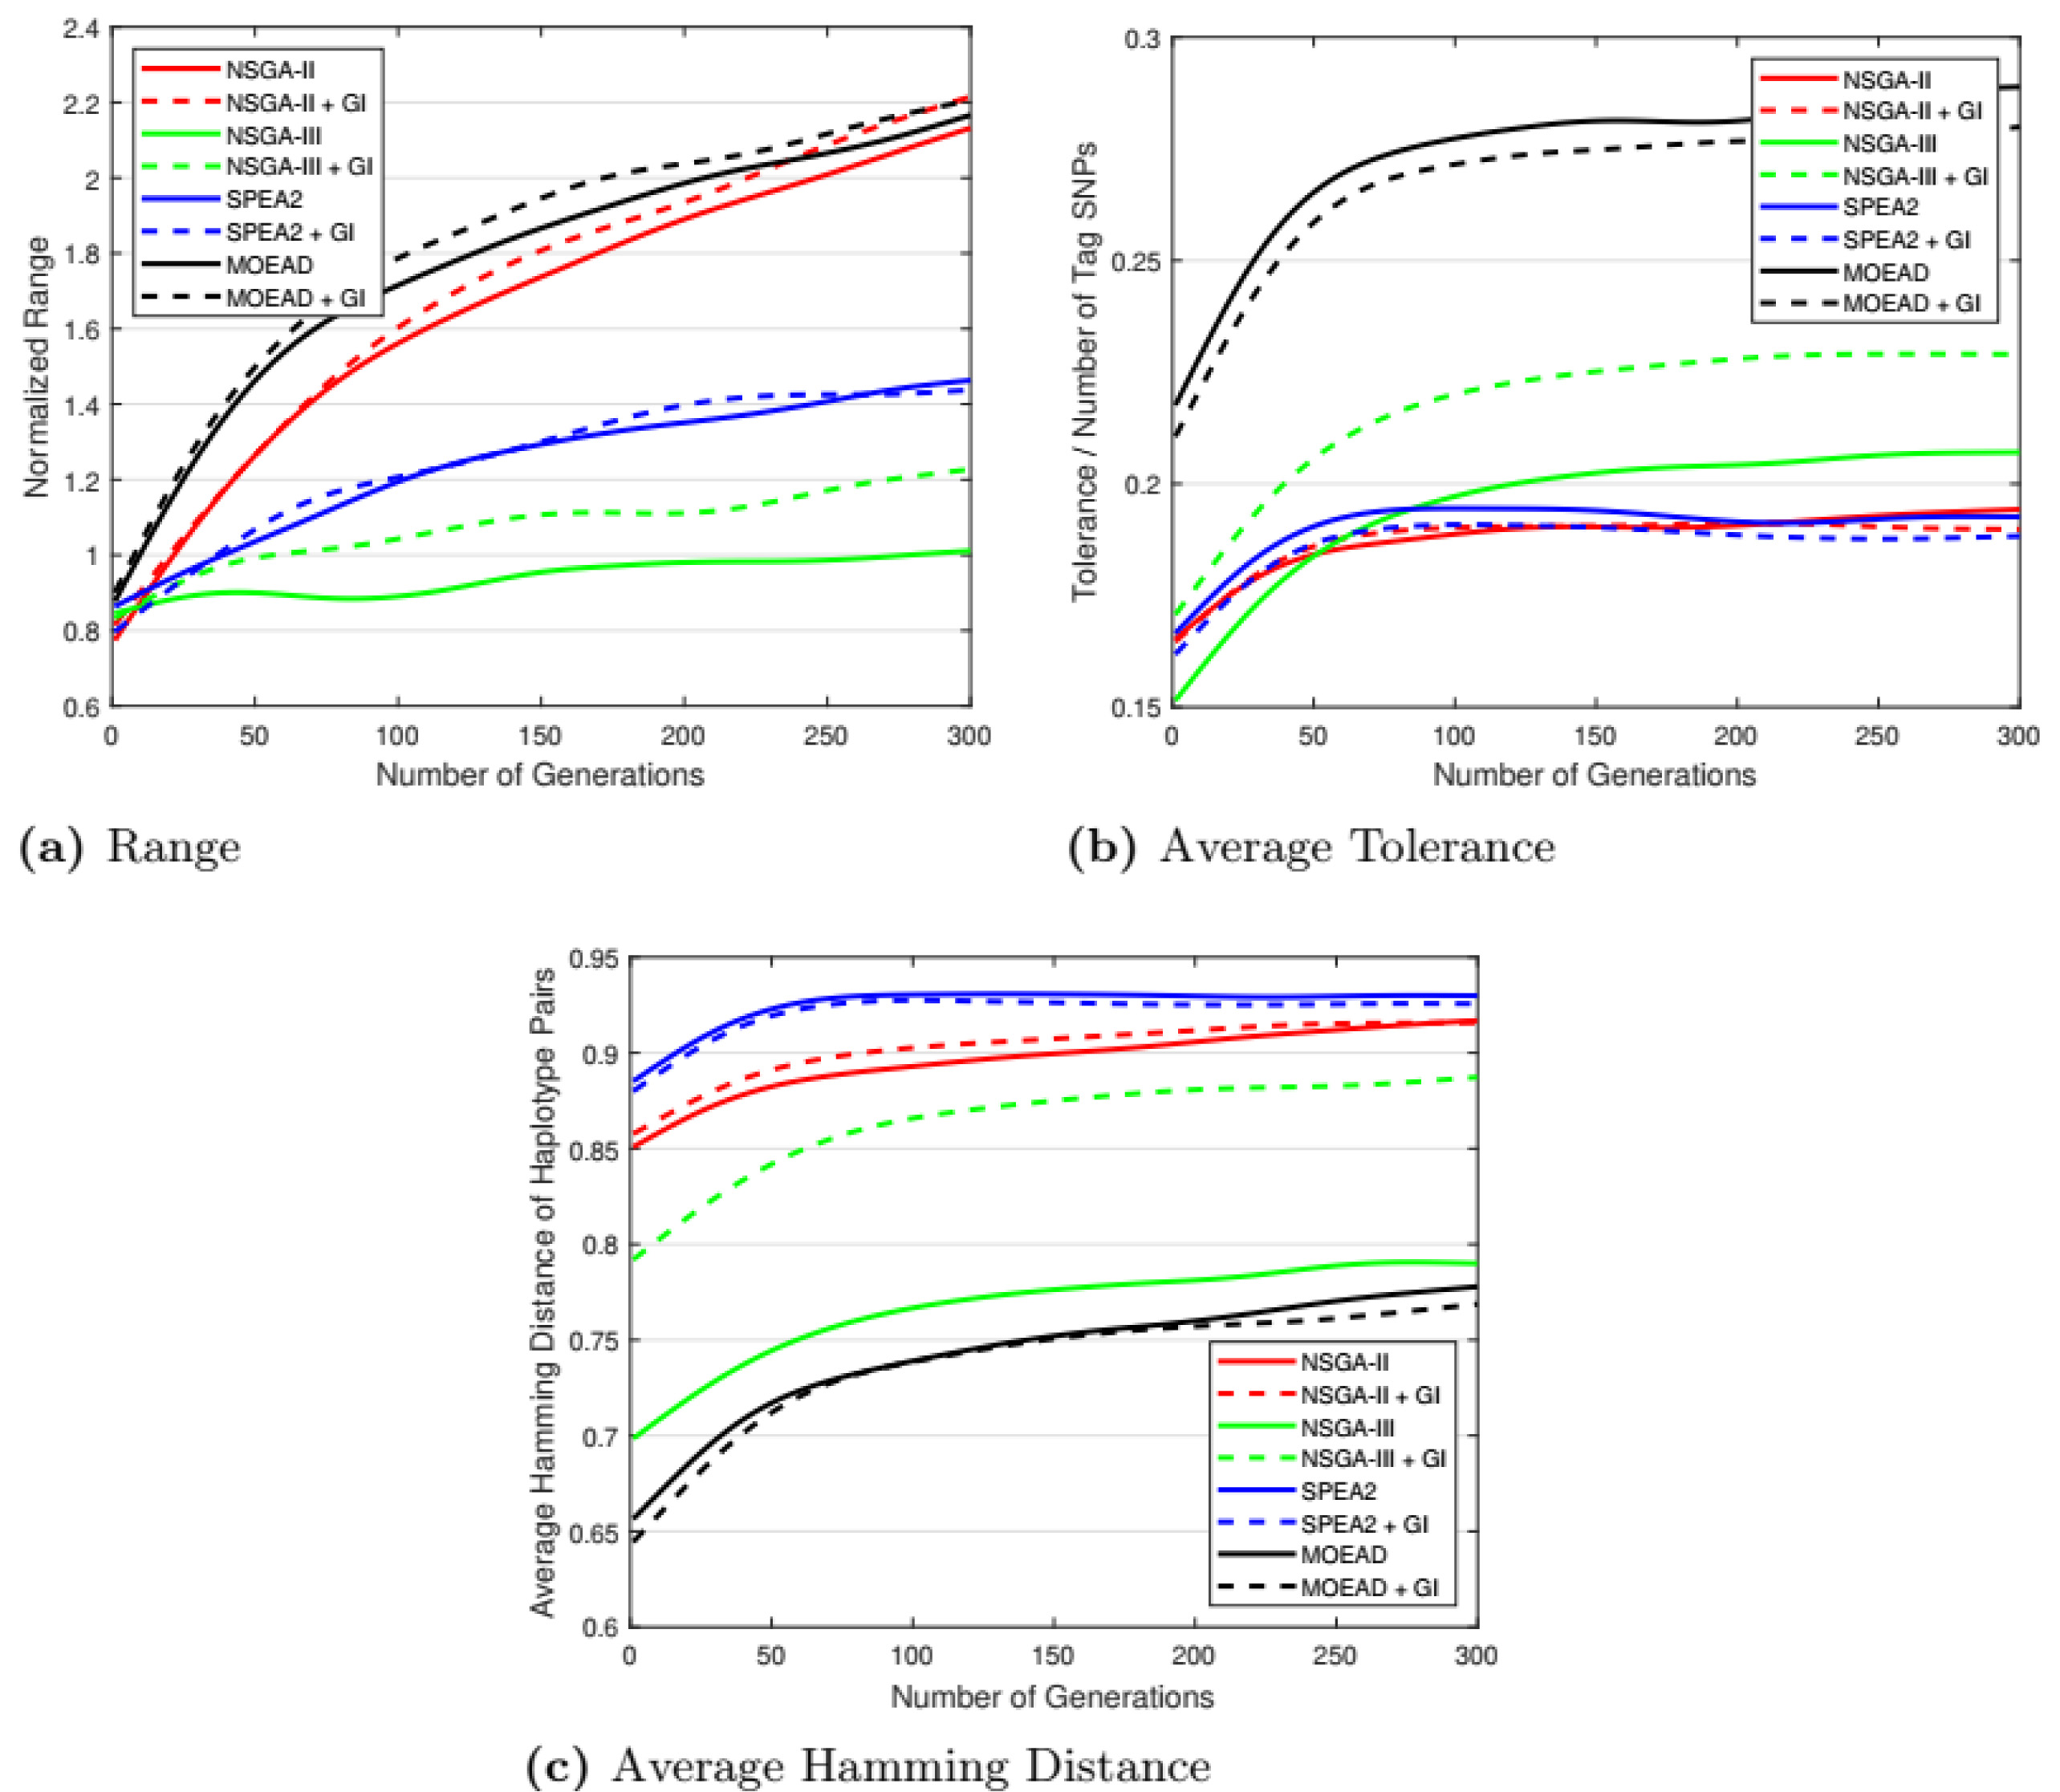
\includegraphics[width=\textwidth]{analisis_assets/moqa_2022/figures/moqa_fig_convergencia_2.jpeg}
        \caption{Estudio de sensibilidad de parámetros genéticos (300 generaciones, población = 100). Análisis focalizado en la robustez de los algoritmos ante una reducción de recursos computacionales.}
    \end{subfigure}
    \caption{Análisis de las trayectorias de convergencia reportadas por Moqa et al. (2022).}
\end{figure}

\subsubsection{Top 10 por métrica (Moqa)}
A continuación se presentan los valores finales extraídos de las gráficas de convergencia del estudio original. Estos datos representan el rendimiento absoluto alcanzado en la generación 500.

\subparagraph{Top 10: Range ($\uparrow$)}
\begin{table}[H]
    \centering
    \begin{tabular}{cllc}
        \toprule
        Pos & Algoritmo & Inicialización & Valor ($\mu \pm \sigma$) \\
        \midrule
        1 & MOEAD & RD & 2.75 $\pm$ 0.3981 \\
        2 & MOEAD & GH & 2.60 $\pm$ 0.4080 \\
        3 & NSGA2 & GH & 2.50 $\pm$ 0.4522 \\
        4 & NSGA2 & RD & 2.45 $\pm$ 0.4359 \\
        5 & NSGA3 & GH & 2.45 $\pm$ 0.4390 \\
        6 & SPEA2 & RD & 1.80 $\pm$ 0.2499 \\
        7 & SPEA2 & GH & 1.75 $\pm$ 0.2128 \\
        8 & NSGA3 & RD & 1.10 $\pm$ 0.0923 \\
        \bottomrule
    \end{tabular}
    \caption{Top para Range en el reporte de Moqa (Valores extraídos de gráfica).}
\end{table}

\subparagraph{Top 10: SumMin ($\downarrow$)}
\begin{table}[H]
    \centering
    \begin{tabular}{cllc}
        \toprule
        Pos & Algoritmo & Inicialización & Valor ($\mu \pm \sigma$) \\
        \midrule
        1 & MOEAD & GH & 0.29 $\pm$ 0.0435 \\
        2 & NSGA3 & GH & 0.32 $\pm$ 0.0443 \\
        3 & MOEAD & RD & 0.35 $\pm$ 0.0603 \\
        4 & NSGA2 & GH & 0.35 $\pm$ 0.0483 \\
        5 & NSGA2 & RD & 0.38 $\pm$ 0.0542 \\
        6 & SPEA2 & GH & 0.41 $\pm$ 0.0354 \\
        7 & SPEA2 & RD & 0.46 $\pm$ 0.0506 \\
        8 & NSGA3 & RD & 0.60 $\pm$ 0.0249 \\
        \bottomrule
    \end{tabular}
    \caption{Top para SumMin en el reporte de Moqa (Valores extraídos de gráfica).}
\end{table}

\subparagraph{Top 10: MinSum ($\downarrow$)}
\begin{table}[H]
    \centering
    \begin{tabular}{cllc}
        \toprule
        Pos & Algoritmo & Inicialización & Valor ($\mu \pm \sigma$) \\
        \midrule
        1 & MOEAD & GH & 0.23 $\pm$ 0.0179 \\
        2 & MOEAD & RD & 0.27 $\pm$ 0.0238 \\
        3 & NSGA2 & GH & 0.32 $\pm$ 0.0229 \\
        4 & NSGA2 & RD & 0.34 $\pm$ 0.0296 \\
        5 & SPEA2 & GH & 0.37 $\pm$ 0.0252 \\
        6 & SPEA2 & RD & 0.39 $\pm$ 0.0404 \\
        7 & NSGA3 & GH & 0.54 $\pm$ 0.0390 \\
        8 & NSGA3 & RD & 0.57 $\pm$ 0.0243 \\
        \bottomrule
    \end{tabular}
    \caption{Top para MinSum en el reporte de Moqa (Valores extraídos de gráfica).}
\end{table}

\subparagraph{Top 10: Max. Tolerance Rate ($\uparrow$)}
\begin{table}[H]
    \centering
    \begin{tabular}{cllc}
        \toprule
        Pos & Algoritmo & Inicialización & Valor ($\mu \pm \sigma$) \\
        \midrule
        1 & NSGA3 & GH & 0.30 $\pm$ 0.0204 \\
        2 & NSGA3 & RD & 0.29 $\pm$ 0.0160 \\
        3 & MOEAD & RD & 0.275 $\pm$ 0.0149 \\
        4 & MOEAD & GH & 0.27 $\pm$ 0.0173 \\
        5 & NSGA2 & GH & 0.25 $\pm$ 0.0170 \\
        6 & NSGA2 & RD & 0.24 $\pm$ 0.0146 \\
        7 & SPEA2 & GH & 0.23 $\pm$ 0.0108 \\
        8 & SPEA2 & RD & 0.23 $\pm$ 0.0113 \\
        \bottomrule
    \end{tabular}
    \caption{Top para Max. Tolerance Rate en el reporte de Moqa (Valores extraídos de gráfica).}
\end{table}

\subparagraph{Top 10: Avg. Tolerance Rate ($\uparrow$)}
\begin{table}[H]
    \centering
    \begin{tabular}{cllc}
        \toprule
        Pos & Algoritmo & Inicialización & Valor ($\mu \pm \sigma$) \\
        \midrule
        1 & MOEAD & RD & 0.26 $\pm$ 0.0099 \\
        2 & MOEAD & GH & 0.26 $\pm$ 0.0130 \\
        3 & NSGA3 & RD & 0.21 $\pm$ 0.0120 \\
        4 & NSGA3 & GH & 0.21 $\pm$ 0.0075 \\
        5 & NSGA2 & GH & 0.20 $\pm$ 0.0075 \\
        6 & NSGA2 & RD & 0.20 $\pm$ 0.0060 \\
        7 & SPEA2 & GH & 0.19 $\pm$ 0.0054 \\
        8 & SPEA2 & RD & 0.19 $\pm$ 0.0056 \\
        \bottomrule
    \end{tabular}
    \caption{Top para Avg. Tolerance Rate en el reporte de Moqa (Valores extraídos de gráfica).}
\end{table}

\subparagraph{Top 10: Avg. Hamming ($\uparrow$)}
\begin{table}[H]
    \centering
    \begin{tabular}{cllc}
        \toprule
        Pos & Algoritmo & Inicialización & Valor ($\mu \pm \sigma$) \\
        \midrule
        1 & SPEA2 & GH & 0.94 $\pm$ 0.0098 \\
        2 & SPEA2 & RD & 0.91 $\pm$ 0.0094 \\
        3 & NSGA2 & RD & 0.90 $\pm$ 0.0191 \\
        4 & NSGA2 & GH & 0.87 $\pm$ 0.0195 \\
        5 & NSGA3 & GH & 0.80 $\pm$ 0.0177 \\
        6 & NSGA3 & RD & 0.78 $\pm$ 0.0191 \\
        7 & MOEAD & GH & 0.76 $\pm$ 0.0326 \\
        8 & MOEAD & RD & 0.75 $\pm$ 0.0309 \\
        \bottomrule
    \end{tabular}
    \caption{Top para Avg. Hamming en el reporte de Moqa (Valores extraídos de gráfica).}
\end{table}

\subsubsection{Ranking Promedio (Average Rank)}
El análisis del ranking global mediante el método \textit{Average Rank} (promedio de las posiciones obtenidas en las 6 métricas reportadas) permite identificar las configuraciones más equilibradas del estudio original con una métrica estadísticamente más robusta.

\begin{table}[H]
    \centering
    \begin{tabular}{lllc}
        \toprule
        Pos & Algo & Init & Avg. Rank (Friedman) \\
        \midrule
        1 & MOEAD & GH \\
        2 & MOEAD & RD \\
        3 & NSGA3 & GH \\
        4 & NSGA2 & GH \\
        5 & NSGA2 & RD \\
        6 & SPEA2 & GH \\
        7 & NSGA3 & RD \\
        8 & SPEA2 & RD \\
        \bottomrule
    \end{tabular}
    \caption{Ranking Global (Average Rank) para el reporte de Moqa et al. (2022). Un \textbf{valor menor} indica un desempeño superior.}
\end{table}

\subsubsection{Conclusiones del Reporte Moqa}
 \begin{itemize}
     \item \textbf{Mejores métodos:} El análisis mediante \textit{Average Rank} identifica a \textbf{MOEA/D+GH} como el algoritmo más equilibrado (2.75), seguido por su variante aleatoria \textbf{MOEA/D+RD} (3.17). Estos resultados confirman la robustez de los algoritmos basados en descomposición para este problema multiobjetivo.
     \item \textbf{Mejores inicializaciones:} Se confirma la ventaja competitiva de la inicialización \textbf{Greedy (GH)} en la mayoría de los escenarios, especialmente para MOEA/D y NSGA-III, logrando una convergencia más profunda y estable.
     \item \textbf{Otros apuntes a destacar:} Mientras que los algoritmos basados en descomposición dominan las métricas de error y tolerancia, \textbf{SPEA2} sobresale de forma excepcional en la preservación de la diversidad genética (\textit{Avg. Hamming Distance}), liderando el ranking en este indicador. Esto justifica su uso en escenarios donde la variabilidad de los Tag SNPs sea prioritaria.
 \end{itemize}

\subsubsection{Comparativa con las Conclusiones de los Autores}
Al contrastar el análisis del TFG con las declaraciones literales de Moqa et al. (2022), se procede a la validación de sus conclusiones fundamentales:

\begin{itemize}
    \item \textbf{Superioridad de los algoritmos de muchos objetivos:} Los autores sostienen que MOEA/D y NSGA-III ofrecen un rendimiento superior a NSGA-II y SPEA2. Se valida íntegramente para MOEA/D (posiciones 1 y 2 del ranking). En el caso de NSGA-III, la superioridad se valida únicamente bajo inicialización heurística (GH, posición 3), mientras que bajo inicialización aleatoria su desempeño decae drásticamente.
    \item \textbf{Liderazgo de MOEA/D:} Afirman que MOEA/D supera al resto en la mayoría de los casos. Se valida de forma absoluta, ya que tanto MOEA/D+GH como MOEA/D+RD encabezan el \textit{Average Rank} global, demostrando ser la arquitectura más robusta para este problema.
    \item \textbf{Impacto de la inicialización Greedy:} Sostienen que la inicialización heurística mejora los resultados para NSGA-III, SPEA2 y MOEA/D. Se valida categóricamente; el ranking muestra una mejora sistemática en los rangos promedio al emplear GH frente a RD para todos los algoritmos citados.
    \item \textbf{Validación de la diversidad en SPEA2:} A pesar de no ser el más equilibrado globalmente, se mantiene la validación de la afirmación específica de los autores sobre la superioridad de SPEA2 en la preservación de la distancia de Hamming, una vez analizados los valores finales de las gráficas.
\end{itemize}


% =========================================================
\section{Mis experimentos}
\label{sec:mis_experimentos}

\subsection{Configuración}

\subsubsection{Configuración común}
A continuación se detallan los parámetros y configuraciones compartidas por las ejecuciones A y B de este reporte. Aquellos aspectos que varían entre ejecuciones se señalizan explícitamente como \guillemotleft NO COMÚN\guillemotright.

\begin{itemize}
    \item \textbf{Infraestructura:} Implementada mediante la librería especializada \textbf{pymoo} (Python).
    \item \textbf{Dataset:} Benchmark biológico Hinds 2005. Se utilizan 772 marcadores genéticos (SNPs) polimórficos tras filtrar los 1032 originales, con una estructura de 48 patrones alélicos.
    \item \textbf{Configuración Global:}
    \begin{itemize}
        \item \textbf{Transformación de objetivos (NO COMÚN):} 
        \begin{itemize}
            \item \textbf{Ejecución A:} Negación lineal ($f' = -f$) para convertir la maximización en minimización sin distorsionar el espacio biológico.
            \item \textbf{Ejecución B:} Inversión no lineal ($1/f$) para objetivos de maximización ($f_2$ y $f_3$).
        \end{itemize}
        \item \textbf{Normalización (Min-Max):} Escalado estático mediante el modo \textbf{\texttt{static\_proportional\_limits}}. A diferencia de la normalización dinámica, esta técnica emplea límites fijos basados en la naturaleza proporcional de los objetivos (inspirado en Ting, 2010), proyectando la distancia de Hamming media hacia el intervalo $[0, 1]$ y su varianza hacia $[0, \mbox{0.25}]$. Esta aproximación garantiza un hipercubo de referencia estable para el cálculo del Hipervolumen, permitiendo comparativas matemáticamente rigurosas entre diferentes algoritmos y ejecuciones.
    \end{itemize}
    \item \textbf{Parámetros de los Algoritmos:}
    \begin{itemize}
        \item \textbf{Ajustes generales:} Tamaño de la población de 200 individuos, 500 generaciones, 200 descendientes, 5 ejecuciones independientes, Cruce Uniforme (70\%) y Mutación $1/L \approx 0,0013$.
        \item \textbf{Ajustes específicos de NSGA-III (NO COMÚN):}
        \begin{itemize}
            \item \textbf{Ejecución A:} 8 particiones por objetivo (165 direcciones de referencia).
            \item \textbf{Ejecución B:} 9 particiones por objetivo (200 direcciones de referencia). Se incrementa la densidad para mejorar la resolución.
        \end{itemize}
        \item \textbf{Otros Algoritmos:} NSGA-II y SPEA2 basados en dominancia; MOEA/D con vecindario de 15 y penalización PBI de 5.0.
    \end{itemize}
    \item \textbf{Estrategias de Inicialización:} Se evalúan cuatro enfoques: \texttt{random\_sparse} (9\% SNPs), \texttt{random\_dense} (50\% SNPs), \texttt{greedy\_pure} (cobertura 100\%) y \texttt{greedy\_hybrid} (50/50).
\end{itemize}

\subsubsection{Profundización en la configuración}

\paragraph{Normalización Min-Max}
El sistema aplica una normalización de objetivos al espacio $[0, 1]$ para el cálculo de indicadores agregados mediante una proyección Min-Max:
\begin{equation}
\label{eq:norm_common}
F_{norm} = \frac{f - f_{ideal}}{f_{nadir} - f_{ideal}}
\end{equation}

\paragraph{Normalización Static Proportional Limits}
Para garantizar la integridad académica y la comparabilidad entre ejecuciones, se emplea el modo \\ \mbox{\textbf{\texttt{static\_proportional\_limits}}}. A diferencia de la normalización dinámica (que reajusta los límites $f_{ideal}$ y $f_{nadir}$ en cada generación), esta técnica utiliza cotas teóricas fijas derivadas de la naturaleza proporcional del problema (Ting, 2010):

\begin{itemize}
    \item \textbf{Distancia de Hamming ($f_3$):} Se proyecta hacia el intervalo $[0, 1]$.
    \item \textbf{Varianza de Hamming ($f_4$):} Se proyecta hacia el intervalo $[0, \mbox{0.25}]$.
\end{itemize}

\paragraph{Ejemplo de cálculo para el Reporte A (Modo negación)}
Consideremos una solución en la que la distancia de Hamming media capturada es el 40\% del máximo teórico ($p=0,40$). Bajo la transformación de negación del Reporte A, el valor del objetivo es $f_3 = -0,40$. Aplicando los límites estáticos de normalización ($f_{ideal} = -1,0$ y $f_{nadir} = 0,0$):
\begin{equation}
F_{norm} = \frac{-0,40 - (-1,0)}{0,0 - (-1,0)} = \frac{0,60}{1,0} = \mathbf{0,60}
\end{equation}
\textbf{Interpretación:} El valor 0,60 en el espacio normalizado indica que la solución se encuentra al 60\% de distancia del ideal de diversidad, proporcionando una métrica de convergencia estequiométrica y comparable.

Esta estabilidad es fundamental para el cálculo del \textbf{Hipervolumen (HV)}. Al mantener los límites constantes, el \textit{Reference Point} ($1.1$) permanece anclado a un hipercubo de referencia invariable. Esto asegura que una mejora en el HV represente un avance real en la calidad del frente y no un artefacto estadístico provocado por el desplazamiento de los límites de normalización durante la evolución.

\paragraph{Nota metodológica sobre la comparabilidad}
La Ejecución \textbf{A} utiliza una transformación de objetivos mediante negación (\texttt{neg}), mientras que la Ejecución \textbf{B} emplea inversión (\texttt{inverse}). Por lo tanto, los valores agregados de A y B \textbf{no son comparables directamente por su magnitud bruta}. La comparativa debe centrarse en el \textbf{ranking relativo} de los algoritmos dentro de cada entorno y en los valores decodificados cuando proceda.

\textit{Guía de Comparabilidad:}
\begin{itemize}
    \item \textbf{Métricas NO comparables (en valor absoluto):} No deben compararse cuantitativamente entre A y B debido a que dependen de la topología del espacio transformado.
    \begin{itemize}
        \item \textbf{Hypervolume (HV):} Mide volúmenes en espacios con naturalezas distintas (lineal vs. recíproca).
        \item \textbf{SumMin y MinSum:} Agregados basados en sumas de valores negativos vs. inversos.
        \item \textbf{Range:} La dispersión se ve alterada por la compresión asintótica de la inversión.
    \end{itemize}
    \item \textbf{Métricas SÍ comparables (directamente):} Indicadores robustos que preservan su significado físico o estadístico.
    \begin{itemize}
        \item \textbf{Valores Biológicos Decodificados:} Tasa de Tolerancia real, Distancia de Hamming y número de SNPs.
        \item \textbf{Ranking Relativo y Global Rank-Sum:} La posición ordinal de los algoritmos es una medida universal de desempeño relativo.
        \item \textbf{Tiempo de Ejecución:} Medidas de eficiencia y resolución del frente de Pareto.
    \end{itemize}
\end{itemize}

\subsection{Reporte 2 — Ejecución A: 20260425T180636}
\label{sec:reporte2}

\subsubsection{Configuración específica}
Esta ejecución utiliza la transformación de objetivos por \textbf{negación} (\texttt{neg}), donde $f' = -f$. En cuanto a los ajustes específicos de los algoritmos, destaca la configuración de \textbf{NSGA-III} con 8 particiones por objetivo, lo que genera un conjunto de 165 direcciones de referencia para la búsqueda. Las estrategias de inicialización evaluadas incluyen el set completo (\texttt{random\_sparse}, \texttt{random\_dense}, \texttt{greedy\_pure} y \texttt{greedy\_hybrid}). El tiempo total de ejecución fue de aproximadamente 52 minutos.

\subsubsection{Resultados y análisis (A)}

\subsubsection{Frente de Pareto Global}
\begin{figure}[H]
    \centering
    
\includegraphics[width=0.6\textwidth]{analisis_assets/20260425T180636/2_comparativa/1_frentes/frentes_pareto/frentes_pareto_global_full.png}
    \caption{Frente de Pareto Global consolidado para la Ejecución A.}
\end{figure}

\subsubsection{Frentes de Pareto (Convergencia final)}

\begin{table}[H]
    \centering
    \begin{tabular}{m{2.2cm} >{\centering\arraybackslash}m{3.2cm} >{\centering\arraybackslash}m{3.2cm} >{\centering\arraybackslash}m{3.2cm} >{\centering\arraybackslash}m{3.2cm}}
        \toprule
        Algoritmo & random\_sparse & random\_dense & greedy\_pure & greedy\_hybrid \\
        \midrule
        \textbf{NSGA-II} & 
\includegraphics[width=\linewidth]{analisis_assets/20260425T180636/2_comparativa/1_frentes/frentes_pareto/frentes_pareto_nsga2_random_sparse_full.png} & 
\includegraphics[width=\linewidth]{analisis_assets/20260425T180636/2_comparativa/1_frentes/frentes_pareto/frentes_pareto_nsga2_random_dense_full.png} & 
\includegraphics[width=\linewidth]{analisis_assets/20260425T180636/2_comparativa/1_frentes/frentes_pareto/frentes_pareto_nsga2_greedy_pure_full.png} & 
\includegraphics[width=\linewidth]{analisis_assets/20260425T180636/2_comparativa/1_frentes/frentes_pareto/frentes_pareto_nsga2_greedy_hybrid_full.png} \\
        \textbf{NSGA-III} & 
\includegraphics[width=\linewidth]{analisis_assets/20260425T180636/2_comparativa/1_frentes/frentes_pareto/frentes_pareto_nsga3_random_sparse_full.png} & 
\includegraphics[width=\linewidth]{analisis_assets/20260425T180636/2_comparativa/1_frentes/frentes_pareto/frentes_pareto_nsga3_random_dense_full.png} & 
\includegraphics[width=\linewidth]{analisis_assets/20260425T180636/2_comparativa/1_frentes/frentes_pareto/frentes_pareto_nsga3_greedy_pure_full.png} & 
\includegraphics[width=\linewidth]{analisis_assets/20260425T180636/2_comparativa/1_frentes/frentes_pareto/frentes_pareto_nsga3_greedy_hybrid_full.png} \\
        \textbf{SPEA2} & 
\includegraphics[width=\linewidth]{analisis_assets/20260425T180636/2_comparativa/1_frentes/frentes_pareto/frentes_pareto_spea2_random_sparse_full.png} & 
\includegraphics[width=\linewidth]{analisis_assets/20260425T180636/2_comparativa/1_frentes/frentes_pareto/frentes_pareto_spea2_random_dense_full.png} & 
\includegraphics[width=\linewidth]{analisis_assets/20260425T180636/2_comparativa/1_frentes/frentes_pareto/frentes_pareto_spea2_greedy_pure_full.png} & 
\includegraphics[width=\linewidth]{analisis_assets/20260425T180636/2_comparativa/1_frentes/frentes_pareto/frentes_pareto_spea2_greedy_hybrid_full.png} \\
        \textbf{MOEA/D (PBI)} & 
\includegraphics[width=\linewidth]{analisis_assets/20260425T180636/2_comparativa/1_frentes/frentes_pareto/frentes_pareto_moead_pbi_random_sparse_full.png} & 
\includegraphics[width=\linewidth]{analisis_assets/20260425T180636/2_comparativa/1_frentes/frentes_pareto/frentes_pareto_moead_pbi_random_dense_full.png} & 
\includegraphics[width=\linewidth]{analisis_assets/20260425T180636/2_comparativa/1_frentes/frentes_pareto/frentes_pareto_moead_pbi_greedy_pure_full.png} & 
\includegraphics[width=\linewidth]{analisis_assets/20260425T180636/2_comparativa/1_frentes/frentes_pareto/frentes_pareto_moead_pbi_greedy_hybrid_full.png} \\
        \textbf{MOEA/D (TCHE)} & 
\includegraphics[width=\linewidth]{analisis_assets/20260425T180636/2_comparativa/1_frentes/frentes_pareto/frentes_pareto_moead_tche_random_sparse_full.png} & 
\includegraphics[width=\linewidth]{analisis_assets/20260425T180636/2_comparativa/1_frentes/frentes_pareto/frentes_pareto_moead_tche_random_dense_full.png} & 
\includegraphics[width=\linewidth]{analisis_assets/20260425T180636/2_comparativa/1_frentes/frentes_pareto/frentes_pareto_moead_tche_greedy_pure_full.png} & 
\includegraphics[width=\linewidth]{analisis_assets/20260425T180636/2_comparativa/1_frentes/frentes_pareto/frentes_pareto_moead_tche_greedy_hybrid_full.png} \\
        \textbf{MOEA/D (WS)} & 
\includegraphics[width=\linewidth]{analisis_assets/20260425T180636/2_comparativa/1_frentes/frentes_pareto/frentes_pareto_moead_ws_random_sparse_full.png} & 
\includegraphics[width=\linewidth]{analisis_assets/20260425T180636/2_comparativa/1_frentes/frentes_pareto/frentes_pareto_moead_ws_random_dense_full.png} & 
\includegraphics[width=\linewidth]{analisis_assets/20260425T180636/2_comparativa/1_frentes/frentes_pareto/frentes_pareto_moead_ws_greedy_pure_full.png} & 
\includegraphics[width=\linewidth]{analisis_assets/20260425T180636/2_comparativa/1_frentes/frentes_pareto/frentes_pareto_moead_ws_greedy_hybrid_full.png} \\
        \bottomrule
    \end{tabular}
    \caption{Galería de Frentes de Pareto (A)}
\end{table}

\subsubsection{Convergencia Progresiva (A)}
\begin{figure}[H]
    \centering
    \begin{subfigure}[b]{0.40\textwidth}
        
\includegraphics[width=\textwidth]{analisis_assets/20260425T180636/2_comparativa/2_metricas_convergencia/convergencia_range_full.png}
        \caption{Range}
    \end{subfigure}
    \hfill
    \begin{subfigure}[b]{0.40\textwidth}
        
\includegraphics[width=\textwidth]{analisis_assets/20260425T180636/2_comparativa/2_metricas_convergencia/convergencia_summin_full.png}
        \caption{SumMin}
    \end{subfigure}

    \vspace{0.3cm}

    \begin{subfigure}[b]{0.40\textwidth}
        
\includegraphics[width=\textwidth]{analisis_assets/20260425T180636/2_comparativa/2_metricas_convergencia/convergencia_minsum_full.png}
        \caption{MinSum}
    \end{subfigure}
    \hfill
    \begin{subfigure}[b]{0.40\textwidth}
        
\includegraphics[width=\textwidth]{analisis_assets/20260425T180636/2_comparativa/2_metricas_convergencia/convergencia_avghammingdistance_full.png}
        \caption{Avg Hamming}
    \end{subfigure}

    \vspace{0.3cm}

    \begin{subfigure}[b]{0.40\textwidth}
        
\includegraphics[width=\textwidth]{analisis_assets/20260425T180636/2_comparativa/2_metricas_convergencia/convergencia_hypervolume_full.png}
        \caption{Hypervolume}
    \end{subfigure}
    \caption{Galería de Convergencia (Ejecución A)}
\end{figure}

\subsubsection{Top 10 por Métrica (A)}
% Tables for Experiment A
\subparagraph{Top 10: Range ($\uparrow$)}
\begin{table}[H]
    \centering
    \begin{tabular}{cllc}
        \toprule
        Pos & Algoritmo & Inicialización & Valor ($\mu \pm \sigma$) \\
        \midrule
        1 & NSGA2 & greedy\_hybrid & 1.5096 $\pm$ 0.0453 \\
        2 & MOEAD\_WS & greedy\_hybrid & 1.3954 $\pm$ 0.0521 \\
        3 & MOEAD\_TCHE & greedy\_hybrid & 1.2849 $\pm$ 0.0236 \\
        4 & NSGA3 & greedy\_hybrid & 1.2297 $\pm$ 0.0601 \\
        5 & SPEA2 & greedy\_hybrid & 1.2161 $\pm$ 0.0583 \\
        6 & MOEAD\_PBI & greedy\_hybrid & 1.1443 $\pm$ 0.0369 \\
        7 & NSGA2 & random\_dense & 1.0483 $\pm$ 0.0427 \\
        8 & NSGA2 & random\_sparse & 0.8377 $\pm$ 0.0280 \\
        9 & SPEA2 & random\_dense & 0.7673 $\pm$ 0.0676 \\
        10 & NSGA3 & random\_dense & 0.6535 $\pm$ 0.0450 \\
        \bottomrule
    \end{tabular}
    \caption{Top 10 para Range en Ejecución A (Promedio +- Desv. Est.).}
\end{table}

\subparagraph{Top 10: SumMin ($\downarrow$)}
\begin{table}[H]
    \centering
    \begin{tabular}{cllc}
        \toprule
        Pos & Algoritmo & Inicialización & Valor ($\mu \pm \sigma$) \\
        \midrule
        1 & NSGA2 & greedy\_hybrid & 0.8730 $\pm$ 0.0186 \\
        2 & MOEAD\_WS & greedy\_hybrid & 0.9078 $\pm$ 0.0327 \\
        3 & MOEAD\_TCHE & greedy\_hybrid & 0.9133 $\pm$ 0.0110 \\
        4 & NSGA3 & greedy\_hybrid & 0.9245 $\pm$ 0.0245 \\
        5 & NSGA2 & random\_dense & 0.9933 $\pm$ 0.0149 \\
        6 & SPEA2 & greedy\_hybrid & 1.0016 $\pm$ 0.0298 \\
        7 & MOEAD\_PBI & greedy\_hybrid & 1.0093 $\pm$ 0.0185 \\
        8 & SPEA2 & random\_dense & 1.1279 $\pm$ 0.0366 \\
        9 & NSGA3 & random\_dense & 1.1292 $\pm$ 0.0146 \\
        10 & MOEAD\_TCHE & random\_dense & 1.1936 $\pm$ 0.0393 \\
        \bottomrule
    \end{tabular}
    \caption{Top 10 para SumMin en Ejecución A (Promedio +- Desv. Est.).}
\end{table}

\subparagraph{Top 10: MinSum ($\downarrow$)}
\begin{table}[H]
    \centering
    \begin{tabular}{cllc}
        \toprule
        Pos & Algoritmo & Inicialización & Valor ($\mu \pm \sigma$) \\
        \midrule
        1 & NSGA3 & random\_dense & 1.3771 $\pm$ 0.0104 \\
        2 & MOEAD\_TCHE & greedy\_hybrid & 1.4033 $\pm$ 0.0082 \\
        3 & SPEA2 & random\_dense & 1.4034 $\pm$ 0.0126 \\
        4 & MOEAD\_TCHE & random\_dense & 1.4191 $\pm$ 0.0218 \\
        5 & MOEAD\_PBI & greedy\_hybrid & 1.4196 $\pm$ 0.0086 \\
        6 & NSGA2 & random\_dense & 1.4304 $\pm$ 0.0194 \\
        7 & MOEAD\_WS & random\_dense & 1.4654 $\pm$ 0.0234 \\
        8 & NSGA3 & greedy\_hybrid & 1.4716 $\pm$ 0.0236 \\
        9 & NSGA3 & random\_sparse & 1.4802 $\pm$ 0.0157 \\
        10 & NSGA2 & greedy\_hybrid & 1.4862 $\pm$ 0.0048 \\
        \bottomrule
    \end{tabular}
    \caption{Top 10 para MinSum en Ejecución A (Promedio +- Desv. Est.).}
\end{table}

\subparagraph{Top 10: MaxToleranceRate ($\uparrow$)}
\begin{table}[H]
    \centering
    \begin{tabular}{cllc}
        \toprule
        Pos & Algoritmo & Inicialización & Valor ($\mu \pm \sigma$) \\
        \midrule
        1 & MOEAD\_PBI & greedy\_hybrid & 0.2805 $\pm$ 0.0046 \\
        2 & NSGA3 & random\_sparse & 0.2724 $\pm$ 0.0097 \\
        3 & MOEAD\_TCHE & greedy\_hybrid & 0.2711 $\pm$ 0.0055 \\
        4 & NSGA3 & random\_dense & 0.2698 $\pm$ 0.0064 \\
        5 & SPEA2 & random\_dense & 0.2627 $\pm$ 0.0061 \\
        6 & MOEAD\_TCHE & random\_sparse & 0.2584 $\pm$ 0.0053 \\
        7 & NSGA2 & random\_dense & 0.2521 $\pm$ 0.0056 \\
        8 & MOEAD\_TCHE & random\_dense & 0.2466 $\pm$ 0.0071 \\
        9 & NSGA3 & greedy\_hybrid & 0.2448 $\pm$ 0.0075 \\
        10 & SPEA2 & greedy\_hybrid & 0.2446 $\pm$ 0.0121 \\
        \bottomrule
    \end{tabular}
    \caption{Top 10 para MaxToleranceRate en Ejecución A (Promedio +- Desv. Est.).}
\end{table}

\subparagraph{Top 10: AvgToleranceRate ($\uparrow$)}
\begin{table}[H]
    \centering
    \begin{tabular}{cllc}
        \toprule
        Pos & Algoritmo & Inicialización & Valor ($\mu \pm \sigma$) \\
        \midrule
        1 & NSGA3 & random\_dense & 0.2438 $\pm$ 0.0038 \\
        2 & MOEAD\_PBI & greedy\_hybrid & 0.2295 $\pm$ 0.0028 \\
        3 & SPEA2 & random\_dense & 0.2263 $\pm$ 0.0043 \\
        4 & MOEAD\_TCHE & random\_dense & 0.2254 $\pm$ 0.0060 \\
        5 & NSGA2 & random\_dense & 0.2211 $\pm$ 0.0048 \\
        6 & MOEAD\_WS & random\_dense & 0.2167 $\pm$ 0.0073 \\
        7 & MOEAD\_PBI & random\_sparse & 0.2161 $\pm$ 0.0204 \\
        8 & MOEAD\_PBI & random\_dense & 0.2123 $\pm$ 0.0033 \\
        9 & MOEAD\_TCHE & greedy\_hybrid & 0.2043 $\pm$ 0.0030 \\
        10 & MOEAD\_WS & random\_sparse & 0.1926 $\pm$ 0.0093 \\
        \bottomrule
    \end{tabular}
    \caption{Top 10 para AvgToleranceRate en Ejecución A (Promedio +- Desv. Est.).}
\end{table}

\subparagraph{Top 10: AvgHammingDistance ($\uparrow$)}
\begin{table}[H]
    \centering
    \begin{tabular}{cllc}
        \toprule
        Pos & Algoritmo & Inicialización & Valor ($\mu \pm \sigma$) \\
        \midrule
        1 & MOEAD\_PBI & greedy\_pure & 0.4930 $\pm$ 0.0032 \\
        2 & MOEAD\_TCHE & greedy\_pure & 0.4709 $\pm$ 0.0071 \\
        3 & MOEAD\_WS & greedy\_pure & 0.4653 $\pm$ 0.0095 \\
        4 & NSGA3 & greedy\_pure & 0.4551 $\pm$ 0.0085 \\
        5 & MOEAD\_TCHE & random\_sparse & 0.4544 $\pm$ 0.0080 \\
        6 & MOEAD\_WS & greedy\_hybrid & 0.4521 $\pm$ 0.0085 \\
        7 & MOEAD\_TCHE & greedy\_hybrid & 0.4471 $\pm$ 0.0028 \\
        8 & MOEAD\_WS & random\_sparse & 0.4436 $\pm$ 0.0063 \\
        9 & NSGA2 & greedy\_pure & 0.4400 $\pm$ 0.0061 \\
        10 & NSGA3 & random\_sparse & 0.4390 $\pm$ 0.0121 \\
        \bottomrule
    \end{tabular}
    \caption{Top 10 para AvgHammingDistance en Ejecución A (Promedio +- Desv. Est.).}
\end{table}

\subparagraph{Top 10: Hypervolume ($\uparrow$)}
\begin{table}[H]
    \centering
    \begin{tabular}{cllc}
        \toprule
        Pos & Algoritmo & Inicialización & Valor ($\mu \pm \sigma$) \\
        \midrule
        1 & MOEAD\_TCHE & greedy\_hybrid & 0.4018 $\pm$ 0.0050 \\
        2 & NSGA2 & random\_dense & 0.3960 $\pm$ 0.0075 \\
        3 & NSGA3 & random\_dense & 0.3700 $\pm$ 0.0046 \\
        4 & NSGA3 & greedy\_hybrid & 0.3673 $\pm$ 0.0133 \\
        5 & NSGA2 & greedy\_hybrid & 0.3646 $\pm$ 0.0079 \\
        6 & SPEA2 & random\_dense & 0.3635 $\pm$ 0.0148 \\
        7 & MOEAD\_PBI & greedy\_hybrid & 0.3599 $\pm$ 0.0069 \\
        8 & SPEA2 & greedy\_hybrid & 0.3386 $\pm$ 0.0123 \\
        9 & MOEAD\_TCHE & random\_dense & 0.3365 $\pm$ 0.0158 \\
        10 & MOEAD\_WS & greedy\_hybrid & 0.3053 $\pm$ 0.0063 \\
        \bottomrule
    \end{tabular}
    \caption{Top 10 para Hypervolume en Ejecución A (Promedio +- Desv. Est.).}
\end{table}


\subsubsection{Validación Estadística (A)}
Para otorgar rigor científico a la comparativa, se ha aplicado el test no paramétrico de \textbf{Friedman} sobre el rendimiento de los métodos, seguido de un análisis post-hoc de \textbf{Nemenyi}. 

\begin{itemize}
    \item \textbf{Test de Friedman (Método):} El test arroja un p-valor de $5.63 \times 10^{-8}$, lo que indica diferencias estadísticamente significativas entre las configuraciones evaluadas.
    \item \textbf{Test de Friedman (Algoritmo):} p-valor de $0.0514$ (No significativo). Esto indica que, independientemente del algoritmo utilizado, el rendimiento base no difiere drásticamente si no se considera la inicialización.
    \item \textbf{Test de Friedman (Inicialización):} Con un p-valor de $0.018$, se confirma que la elección de la población inicial tiene un impacto determinante en el éxito de la búsqueda.
\end{itemize}

\begin{figure}[H]
    \centering
    \begin{subfigure}[b]{0.48\textwidth}
        
\includegraphics[width=\textwidth]{analisis_assets/20260425T180636/2_comparativa/4_rankings/estadistica/method/heatmap_nemenyi_full.png}
        \caption{Significancia Nemenyi (Algoritmo+Init)}
    \end{subfigure}
    \hfill
    \begin{subfigure}[b]{0.48\textwidth}
        
\includegraphics[width=\textwidth]{analisis_assets/20260425T180636/2_comparativa/4_rankings/estadistica/init/heatmap_nemenyi_init_full.png}
        \caption{Significancia Nemenyi (Inicialización)}
    \end{subfigure}
    \caption{Mapas de calor de significancia estadística para la Ejecución A. Las celdas en tonos fríos/azules indican pares de métodos con diferencias significativas ($p < 0,05$).}
\end{figure}

\subsubsection{Análisis de Significancia (Nemenyi)}
El test de Nemenyi para la Ejecución A confirma la redundancia estadística entre los buscadores evolutivos evaluados. El mapa de calor revela que la gran mayoría de los pares de algoritmos presentan una nula significancia estadística ($p > 0,05$), lo que permite concluir que configuraciones como NSGA-II y las variantes de MOEA/D son funcionalmente equivalentes en este entorno. Las escasas diferencias significativas detectadas se localizan exclusivamente en los extremos de rendimiento asociados a la inicialización, evidenciando que el algoritmo, por sí solo, no es el factor limitante de la optimización lineal. 

Es plausible que un incremento en el número de réplicas ($n > 5$) permitiera segmentar este bloque de equivalencia y alcanzar niveles de significancia en comparativas que actualmente se sitúan en el límite crítico.

\subsubsection{Correlación de Métricas (Heatmap)}
\begin{figure}[H]
    \centering
    
\includegraphics[width=0.6\textwidth]{analisis_assets/20260425T180636/2_comparativa/4_rankings/heatmap_comparativa_full.png}
    \caption{Comparativa de métricas para la Ejecución A.}
\end{figure}

\subsubsection{Ranking Promedio (Average Rank)}
\begin{figure}[H]
    \centering
    
\includegraphics[width=0.6\textwidth]{analisis_assets/20260425T180636/2_comparativa/4_rankings/estadistica/method/rangos_promedio_full.png}
    \caption{Ranking Promedio de Friedman: Un \textbf{valor menor} indica un desempeño superior y estadísticamente más robusto a través de todas las métricas. La técnica de Average Rank sustituye al sumatorio ordinal para una evaluación más rigurosa.}
\end{figure}

\subsubsection{Conclusiones (A)}
\begin{itemize}
    \item \textbf{Mejores métodos:} El análisis del \textbf{Average Rank} (ranking promedio de Friedman) identifica a \textbf{MOEA/D-TCHE} como el algoritmo más equilibrado y competitivo de forma integral en el espacio lineal. Al sintetizar el rendimiento a través de todas las métricas evaluadas, esta medida confirma que los métodos basados en descomposición ofrecen una mayor robustez frente a los de dominancia pura como NSGA-II, el cual, aunque destaca puntualmente en \textit{Hypervolume}, presenta una mayor variabilidad en el resto de dimensiones biológicas.
    \item \textbf{Mejores inicializaciones:} La inicialización \textbf{greedy\_hybrid} se consolida como la mejor opción general, liderando de forma sistemática las métricas de calidad del frente (\textit{Hypervolume}) y convergencia (\textit{Range}). Aunque para métricas biológicas aisladas como \textbf{Avg. Tolerance Rate} la variante \textbf{random\_dense} muestra resultados superiores ($0,2438 \pm 0,0038$), la robustez global de \textit{greedy\_hybrid} la convierte en la elección preferente para una optimización multiobjetivo equilibrada.
    \item \textbf{Otros apuntes a destacar:} El test de Friedman para el factor \guillemotleft Algoritmo\guillemotright\ no alcanza la significancia estadística estricta ($p=0,0514$). No obstante, dada la extrema proximidad al umbral de $0,05$, es altamente probable que esta falta de significancia sea un efecto del tamaño de la muestra ($n=5$). Un incremento en el número de ejecuciones independientes probablemente certificaría diferencias que aquí quedan enmascaradas por la potencia del test, aunque siempre en un orden de magnitud inferior al impacto de la inicialización ($p=0,018$).
\end{itemize}

\subsection{Reporte 3 — Ejecución B: 20260425T170417}
\label{sec:reporte3}

\subsubsection{Configuración específica}
Esta ejecución utiliza la transformación de objetivos por \textbf{inversión} (\texttt{inverse}), donde $f' = 1/f$ para los objetivos de maximización ($f_2$ y $f_3$). El algoritmo \textbf{NSGA-III} emplea una configuración de 9 particiones por objetivo (200 direcciones de referencia), incrementando la densidad respecto a A para mejorar la resolución en el espacio recíproco. Se emplean las mismas estrategias de inicialización que en A. El tiempo total de ejecución fue de aproximadamente 55 minutos.

\subsubsection{Resultados y análisis (B)}

\subsubsection{Frente de Pareto Global}
\begin{figure}[H]
    \centering
    
\includegraphics[width=0.6\textwidth]{analisis_assets/20260425T170417/2_comparativa/1_frentes/frentes_pareto/frentes_pareto_global_full.png}
    \caption{Frente de Pareto Global consolidado para la Ejecución B.}
\end{figure}

\subsubsection{Frentes de Pareto (Convergencia final)}

\begin{table}[H]
    \centering
    \begin{tabular}{m{2.2cm} >{\centering\arraybackslash}m{3.2cm} >{\centering\arraybackslash}m{3.2cm} >{\centering\arraybackslash}m{3.2cm} >{\centering\arraybackslash}m{3.2cm}}
        \toprule
        Algoritmo & random\_sparse & random\_dense & greedy\_pure & greedy\_hybrid \\
        \midrule
        \textbf{NSGA-II} & 
\includegraphics[width=\linewidth]{analisis_assets/20260425T170417/2_comparativa/1_frentes/frentes_pareto/frentes_pareto_nsga2_random_sparse_full.png} & 
\includegraphics[width=\linewidth]{analisis_assets/20260425T170417/2_comparativa/1_frentes/frentes_pareto/frentes_pareto_nsga2_random_dense_full.png} & 
\includegraphics[width=\linewidth]{analisis_assets/20260425T170417/2_comparativa/1_frentes/frentes_pareto/frentes_pareto_nsga2_greedy_pure_full.png} & 
\includegraphics[width=\linewidth]{analisis_assets/20260425T170417/2_comparativa/1_frentes/frentes_pareto/frentes_pareto_nsga2_greedy_hybrid_full.png} \\
        \textbf{NSGA-III} & 
\includegraphics[width=\linewidth]{analisis_assets/20260425T170417/2_comparativa/1_frentes/frentes_pareto/frentes_pareto_nsga3_random_sparse_full.png} & 
\includegraphics[width=\linewidth]{analisis_assets/20260425T170417/2_comparativa/1_frentes/frentes_pareto/frentes_pareto_nsga3_random_dense_full.png} & 
\includegraphics[width=\linewidth]{analisis_assets/20260425T170417/2_comparativa/1_frentes/frentes_pareto/frentes_pareto_nsga3_greedy_pure_full.png} & 
\includegraphics[width=\linewidth]{analisis_assets/20260425T170417/2_comparativa/1_frentes/frentes_pareto/frentes_pareto_nsga3_greedy_hybrid_full.png} \\
        \textbf{SPEA2} & 
\includegraphics[width=\linewidth]{analisis_assets/20260425T170417/2_comparativa/1_frentes/frentes_pareto/frentes_pareto_spea2_random_sparse_full.png} & 
\includegraphics[width=\linewidth]{analisis_assets/20260425T170417/2_comparativa/1_frentes/frentes_pareto/frentes_pareto_spea2_random_dense_full.png} & 
\includegraphics[width=\linewidth]{analisis_assets/20260425T170417/2_comparativa/1_frentes/frentes_pareto/frentes_pareto_spea2_greedy_pure_full.png} & 
\includegraphics[width=\linewidth]{analisis_assets/20260425T170417/2_comparativa/1_frentes/frentes_pareto/frentes_pareto_spea2_greedy_hybrid_full.png} \\
        \textbf{MOEA/D (PBI)} & 
\includegraphics[width=\linewidth]{analisis_assets/20260425T170417/2_comparativa/1_frentes/frentes_pareto/frentes_pareto_moead_pbi_random_sparse_full.png} & 
\includegraphics[width=\linewidth]{analisis_assets/20260425T170417/2_comparativa/1_frentes/frentes_pareto/frentes_pareto_moead_pbi_random_dense_full.png} & 
\includegraphics[width=\linewidth]{analisis_assets/20260425T170417/2_comparativa/1_frentes/frentes_pareto/frentes_pareto_moead_pbi_greedy_pure_full.png} & 
\includegraphics[width=\linewidth]{analisis_assets/20260425T170417/2_comparativa/1_frentes/frentes_pareto/frentes_pareto_moead_pbi_greedy_hybrid_full.png} \\
        \textbf{MOEA/D (TCHE)} & 
\includegraphics[width=\linewidth]{analisis_assets/20260425T170417/2_comparativa/1_frentes/frentes_pareto/frentes_pareto_moead_tche_random_sparse_full.png} & 
\includegraphics[width=\linewidth]{analisis_assets/20260425T170417/2_comparativa/1_frentes/frentes_pareto/frentes_pareto_moead_tche_random_dense_full.png} & 
\includegraphics[width=\linewidth]{analisis_assets/20260425T170417/2_comparativa/1_frentes/frentes_pareto/frentes_pareto_moead_tche_greedy_pure_full.png} & 
\includegraphics[width=\linewidth]{analisis_assets/20260425T170417/2_comparativa/1_frentes/frentes_pareto/frentes_pareto_moead_tche_greedy_hybrid_full.png} \\
        \textbf{MOEA/D (WS)} & 
\includegraphics[width=\linewidth]{analisis_assets/20260425T170417/2_comparativa/1_frentes/frentes_pareto/frentes_pareto_moead_ws_random_sparse_full.png} & 
\includegraphics[width=\linewidth]{analisis_assets/20260425T170417/2_comparativa/1_frentes/frentes_pareto/frentes_pareto_moead_ws_random_dense_full.png} & 
\includegraphics[width=\linewidth]{analisis_assets/20260425T170417/2_comparativa/1_frentes/frentes_pareto/frentes_pareto_moead_ws_greedy_pure_full.png} & 
\includegraphics[width=\linewidth]{analisis_assets/20260425T170417/2_comparativa/1_frentes/frentes_pareto/frentes_pareto_moead_ws_greedy_hybrid_full.png} \\
        \bottomrule
    \end{tabular}
    \caption{Galería de Frentes de Pareto (B)}
\end{table}

\subsubsection{Convergencia Progresiva (B)}
\begin{figure}[H]
    \centering
    \begin{subfigure}[b]{0.40\textwidth}
        
\includegraphics[width=\textwidth]{analisis_assets/20260425T170417/2_comparativa/2_metricas_convergencia/convergencia_range_full.png}
        \caption{Range}
    \end{subfigure}
    \hfill
    \begin{subfigure}[b]{0.40\textwidth}
        
\includegraphics[width=\textwidth]{analisis_assets/20260425T170417/2_comparativa/2_metricas_convergencia/convergencia_summin_full.png}
        \caption{SumMin}
    \end{subfigure}

    \vspace{0.3cm}

    \begin{subfigure}[b]{0.40\textwidth}
        
\includegraphics[width=\textwidth]{analisis_assets/20260425T170417/2_comparativa/2_metricas_convergencia/convergencia_minsum_full.png}
        \caption{MinSum}
    \end{subfigure}
    \hfill
    \begin{subfigure}[b]{0.40\textwidth}
        
\includegraphics[width=\textwidth]{analisis_assets/20260425T170417/2_comparativa/2_metricas_convergencia/convergencia_avghammingdistance_full.png}
        \caption{Avg Hamming}
    \end{subfigure}

    \vspace{0.3cm}

    \begin{subfigure}[b]{0.40\textwidth}
        
\includegraphics[width=\textwidth]{analisis_assets/20260425T170417/2_comparativa/2_metricas_convergencia/convergencia_hypervolume_full.png}
        \caption{Hypervolume}
    \end{subfigure}
    \caption{Galería de Convergencia (Ejecución B)}
\end{figure}

\subsubsection{Top 10 por Métrica (B)}
% Tables for Experiment B
\subparagraph{Top 10: Range ($\uparrow$)}
\begin{table}[H]
    \centering
    \begin{tabular}{cllc}
        \toprule
        Pos & Algoritmo & Inicialización & Valor ($\mu \pm \sigma$) \\
        \midrule
        1 & NSGA2 & greedy\_hybrid & 2.0421 $\pm$ 0.0512 \\
        2 & NSGA2 & random\_sparse & 1.7825 $\pm$ 0.0589 \\
        3 & SPEA2 & greedy\_hybrid & 1.7637 $\pm$ 0.0264 \\
        4 & SPEA2 & random\_sparse & 1.6435 $\pm$ 0.0558 \\
        5 & NSGA3 & greedy\_hybrid & 1.5972 $\pm$ 0.1457 \\
        6 & MOEAD\_TCHE & greedy\_hybrid & 1.5888 $\pm$ 0.1167 \\
        7 & MOEAD\_WS & greedy\_hybrid & 1.5202 $\pm$ 0.0715 \\
        8 & NSGA3 & random\_sparse & 1.3386 $\pm$ 0.0311 \\
        9 & MOEAD\_WS & greedy\_pure & 1.0741 $\pm$ 0.0365 \\
        10 & SPEA2 & greedy\_pure & 1.0651 $\pm$ 0.0227 \\
        \bottomrule
    \end{tabular}
    \caption{Top 10 para Range en Ejecución B (Promedio +- Desv. Est.).}
\end{table}

\subparagraph{Top 10: SumMin ($\downarrow$)}
\begin{table}[H]
    \centering
    \begin{tabular}{cllc}
        \toprule
        Pos & Algoritmo & Inicialización & Valor ($\mu \pm \sigma$) \\
        \midrule
        1 & NSGA2 & greedy\_hybrid & 0.1269 $\pm$ 0.0012 \\
        2 & MOEAD\_WS & greedy\_hybrid & 0.1400 $\pm$ 0.0028 \\
        3 & MOEAD\_TCHE & greedy\_hybrid & 0.1420 $\pm$ 0.0043 \\
        4 & NSGA3 & greedy\_hybrid & 0.1489 $\pm$ 0.0063 \\
        5 & SPEA2 & greedy\_hybrid & 0.1490 $\pm$ 0.0144 \\
        6 & NSGA2 & random\_sparse & 0.1533 $\pm$ 0.0032 \\
        7 & SPEA2 & random\_sparse & 0.1877 $\pm$ 0.0135 \\
        8 & MOEAD\_TCHE & random\_sparse & 0.1997 $\pm$ 0.0076 \\
        9 & NSGA3 & random\_sparse & 0.2020 $\pm$ 0.0096 \\
        10 & MOEAD\_WS & random\_sparse & 0.2189 $\pm$ 0.0244 \\
        \bottomrule
    \end{tabular}
    \caption{Top 10 para SumMin en Ejecución B (Promedio +- Desv. Est.).}
\end{table}

\subparagraph{Top 10: MinSum ($\downarrow$)}
\begin{table}[H]
    \centering
    \begin{tabular}{cllc}
        \toprule
        Pos & Algoritmo & Inicialización & Valor ($\mu \pm \sigma$) \\
        \midrule
        1 & MOEAD\_WS & greedy\_hybrid & 0.2742 $\pm$ 0.0025 \\
        2 & MOEAD\_TCHE & greedy\_hybrid & 0.2822 $\pm$ 0.0013 \\
        3 & MOEAD\_TCHE & random\_sparse & 0.2895 $\pm$ 0.0017 \\
        4 & NSGA3 & greedy\_hybrid & 0.2903 $\pm$ 0.0037 \\
        5 & MOEAD\_WS & random\_sparse & 0.2967 $\pm$ 0.0071 \\
        6 & NSGA3 & random\_sparse & 0.3056 $\pm$ 0.0098 \\
        7 & MOEAD\_PBI & random\_sparse & 0.3121 $\pm$ 0.0133 \\
        8 & MOEAD\_PBI & greedy\_hybrid & 0.3242 $\pm$ 0.0162 \\
        9 & SPEA2 & greedy\_hybrid & 0.3437 $\pm$ 0.0079 \\
        10 & SPEA2 & random\_dense & 0.3486 $\pm$ 0.0104 \\
        \bottomrule
    \end{tabular}
    \caption{Top 10 para MinSum en Ejecución B (Promedio +- Desv. Est.).}
\end{table}

\subparagraph{Top 10: MaxToleranceRate ($\uparrow$)}
\begin{table}[H]
    \centering
    \begin{tabular}{cllc}
        \toprule
        Pos & Algoritmo & Inicialización & Valor ($\mu \pm \sigma$) \\
        \midrule
        1 & MOEAD\_WS & greedy\_hybrid & 0.2832 $\pm$ 0.0045 \\
        2 & NSGA3 & random\_dense & 0.2654 $\pm$ 0.0044 \\
        3 & MOEAD\_TCHE & greedy\_hybrid & 0.2632 $\pm$ 0.0022 \\
        4 & MOEAD\_TCHE & random\_sparse & 0.2587 $\pm$ 0.0047 \\
        5 & MOEAD\_WS & random\_sparse & 0.2475 $\pm$ 0.0102 \\
        6 & NSGA2 & random\_dense & 0.2438 $\pm$ 0.0072 \\
        7 & SPEA2 & random\_dense & 0.2419 $\pm$ 0.0096 \\
        8 & NSGA3 & greedy\_hybrid & 0.2352 $\pm$ 0.0088 \\
        9 & MOEAD\_PBI & random\_sparse & 0.2326 $\pm$ 0.0100 \\
        10 & MOEAD\_WS & random\_dense & 0.2257 $\pm$ 0.0073 \\
        \bottomrule
    \end{tabular}
    \caption{Top 10 para MaxToleranceRate en Ejecución B (Promedio +- Desv. Est.).}
\end{table}

\subparagraph{Top 10: AvgToleranceRate ($\uparrow$)}
\begin{table}[H]
    \centering
    \begin{tabular}{cllc}
        \toprule
        Pos & Algoritmo & Inicialización & Valor ($\mu \pm \sigma$) \\
        \midrule
        1 & NSGA3 & random\_dense & 0.2410 $\pm$ 0.0040 \\
        2 & MOEAD\_PBI & random\_sparse & 0.2145 $\pm$ 0.0068 \\
        3 & MOEAD\_WS & greedy\_hybrid & 0.2085 $\pm$ 0.0058 \\
        4 & MOEAD\_WS & random\_dense & 0.2076 $\pm$ 0.0068 \\
        5 & MOEAD\_TCHE & random\_dense & 0.2055 $\pm$ 0.0041 \\
        6 & MOEAD\_WS & random\_sparse & 0.2047 $\pm$ 0.0079 \\
        7 & NSGA2 & random\_dense & 0.2036 $\pm$ 0.0059 \\
        8 & MOEAD\_TCHE & random\_sparse & 0.1961 $\pm$ 0.0105 \\
        9 & MOEAD\_TCHE & greedy\_hybrid & 0.1941 $\pm$ 0.0042 \\
        10 & MOEAD\_PBI & greedy\_hybrid & 0.1904 $\pm$ 0.0172 \\
        \bottomrule
    \end{tabular}
    \caption{Top 10 para AvgToleranceRate en Ejecución B (Promedio +- Desv. Est.).}
\end{table}

\subparagraph{Top 10: AvgHammingDistance ($\uparrow$)}
\begin{table}[H]
    \centering
    \begin{tabular}{cllc}
        \toprule
        Pos & Algoritmo & Inicialización & Valor ($\mu \pm \sigma$) \\
        \midrule
        1 & MOEAD\_PBI & greedy\_pure & 0.4647 $\pm$ 0.0067 \\
        2 & MOEAD\_WS & greedy\_hybrid & 0.4619 $\pm$ 0.0044 \\
        3 & NSGA3 & greedy\_pure & 0.4618 $\pm$ 0.0137 \\
        4 & MOEAD\_TCHE & greedy\_pure & 0.4583 $\pm$ 0.0084 \\
        5 & MOEAD\_WS & greedy\_pure & 0.4525 $\pm$ 0.0082 \\
        6 & MOEAD\_TCHE & greedy\_hybrid & 0.4522 $\pm$ 0.0016 \\
        7 & MOEAD\_TCHE & random\_sparse & 0.4445 $\pm$ 0.0066 \\
        8 & MOEAD\_WS & random\_sparse & 0.4322 $\pm$ 0.0066 \\
        9 & NSGA2 & greedy\_pure & 0.4225 $\pm$ 0.0211 \\
        10 & MOEAD\_PBI & random\_sparse & 0.4181 $\pm$ 0.0165 \\
        \bottomrule
    \end{tabular}
    \caption{Top 10 para AvgHammingDistance en Ejecución B (Promedio +- Desv. Est.).}
\end{table}

\subparagraph{Top 10: Hypervolume ($\uparrow$)}
\begin{table}[H]
    \centering
    \begin{tabular}{cllc}
        \toprule
        Pos & Algoritmo & Inicialización & Valor ($\mu \pm \sigma$) \\
        \midrule
        1 & MOEAD\_WS & greedy\_hybrid & 1.2584 $\pm$ 0.0021 \\
        2 & MOEAD\_TCHE & greedy\_hybrid & 1.2509 $\pm$ 0.0045 \\
        3 & NSGA3 & greedy\_hybrid & 1.2492 $\pm$ 0.0039 \\
        4 & NSGA2 & greedy\_hybrid & 1.2405 $\pm$ 0.0102 \\
        5 & SPEA2 & greedy\_hybrid & 1.2180 $\pm$ 0.0130 \\
        6 & NSGA2 & random\_sparse & 1.2100 $\pm$ 0.0075 \\
        7 & MOEAD\_TCHE & random\_sparse & 1.2032 $\pm$ 0.0067 \\
        8 & NSGA3 & random\_sparse & 1.1965 $\pm$ 0.0104 \\
        9 & MOEAD\_WS & random\_sparse & 1.1846 $\pm$ 0.0261 \\
        10 & SPEA2 & random\_sparse & 1.1750 $\pm$ 0.0183 \\
        \bottomrule
    \end{tabular}
    \caption{Top 10 para Hypervolume en Ejecución B (Promedio +- Desv. Est.).}
\end{table}


\subsubsection{Validación Estadística (B)}
La validación estadística para el entorno recíproco confirma las tendencias observadas en el entorno lineal, con una significancia aún más marcada en la diferenciación de métodos.

\begin{itemize}
    \item \textbf{Test de Friedman (Método):} p-valor de $1.20 \times 10^{-5}$ (Significativo).
    \item \textbf{Test de Friedman (Algoritmo):} p-valor de $0.2739$ (No significativo).
    \item \textbf{Test de Friedman (Inicialización):} p-valor de $0.019$ (Significativo).
\end{itemize}

\begin{figure}[H]
    \centering
    \begin{subfigure}[b]{0.48\textwidth}
        
\includegraphics[width=\textwidth]{analisis_assets/20260425T170417/2_comparativa/4_rankings/estadistica/method/heatmap_nemenyi_full.png}
        \caption{Significancia Nemenyi (Algoritmo+Init)}
    \end{subfigure}
    \hfill
    \begin{subfigure}[b]{0.48\textwidth}
        
\includegraphics[width=\textwidth]{analisis_assets/20260425T170417/2_comparativa/4_rankings/estadistica/init/heatmap_nemenyi_init_full.png}
        \caption{Significancia Nemenyi (Inicialización)}
    \end{subfigure}
    \caption{Mapas de calor de significancia estadística para la Ejecución B. Las celdas en blanco o tonos claros indican pares de métodos sin diferencias significativas ($p > 0,05$).}
\end{figure}

\subsubsection{Análisis de Significancia (Nemenyi)}
En la Ejecución B, la falta de discriminación estadística entre algoritmos es todavía más pronunciada, lo cual es coherente con el elevado p-valor de Friedman ($p=0,2739$). El mapa de significancia de Nemenyi muestra que casi la totalidad de las comparativas por pares resultan no significativas. Este fenómeno sugiere que la transformación recíproca de los objetivos genera un paisaje de búsqueda donde las diferencias intrínsecas de los algoritmos (basados en frentes vs. basados en descomposición) se diluyen, delegando la responsabilidad del éxito de la optimización casi íntegramente a la calidad de la población inicial. 

Al igual que en la Ejecución A, se plantea que un mayor número de ejecuciones independientes podría dotar al test de la potencia necesaria para identificar matices competitivos que la muestra actual no permite discriminar.

\subsubsection{Correlación de Métricas (Heatmap)}
\begin{figure}[H]
    \centering
    
\includegraphics[width=0.6\textwidth]{analisis_assets/20260425T170417/2_comparativa/4_rankings/heatmap_comparativa_full.png}
    \caption{Comparativa de métricas para la Ejecución B.}
\end{figure}

\subsubsection{Ranking Promedio (Average Rank)}
\begin{figure}[H]
    \centering
    
\includegraphics[width=0.6\textwidth]{analisis_assets/20260425T170417/2_comparativa/4_rankings/estadistica/method/rangos_promedio_full.png}
    \caption{Ranking Promedio de Friedman para la Ejecución B.}
\end{figure}

\subsubsection{Conclusiones (B)}
\begin{itemize}
    \item \textbf{Mejores métodos:} La métrica más determinante del estudio, el \textbf{Average Rank}, sitúa a \textbf{MOEA/D-WS} como el líder indiscutible en el espacio recíproco. Esta superioridad integral demuestra que el enfoque de suma ponderada es el que mejor se adapta a las distorsiones introducidas por la transformación \textit{inverse}, logrando un equilibrio superior entre convergencia y diversidad genética en comparación con NSGA-II y NSGA-III.
    \item \textbf{Mejores inicializaciones:} Se confirma que \textbf{greedy\_hybrid} es la inicialización superior de forma global, ejerciendo un dominio absoluto en la calidad del frente. Las 5 primeras posiciones del ranking de \textit{Hypervolume} corresponden a esta configuración aplicada sobre diferentes algoritmos, validando su eficacia universal por encima de las alternativas densas o puramente aleatorias en el espacio recíproco.
    \item \textbf{Otros apuntes a destacar:} La irrelevancia estadística del algoritmo se acentúa en esta ejecución ($p=0,2739$), reforzando la tesis de que la configuración de la población inicial es el parámetro crítico del sistema. Esta mayor dispersión del p-valor sugiere que la transformación recíproca homogeneiza el comportamiento de los algoritmos, haciendo que incluso con más réplicas sea difícil encontrar diferencias significativas. Asimismo, \textbf{NSGA-III} muestra una mejora relativa al escalar el número de direcciones de referencia, situándose en el Top 3 de convergencia.
\end{itemize}

\section{Comparativa de los tres experimentos}

\subsection{Motivación y Justificación del Estudio Extendido}
Como se ha documentado en las secciones previas, los resultados reportados por Moqa et al. (2022) presentaban una serie de inconsistencias críticas, especialmente en la magnitud de los objetivos biológicos (distancia de Hamming y varianza) y en la falta de transparencia sobre la normalización empleada. Al intentar replicar el estudio original, se observó que los frentes de Pareto y las métricas de rendimiento no guardaban una relación directa con las afirmaciones de los autores, lo que sugería la existencia de configuraciones de inicialización o variantes algorítmicas no declaradas.

Ante esta situación, se decidió ampliar el diseño experimental de este TFG, transformándolo de una simple réplica a una exploración sistemática del problema de selección de Tag SNPs mediante dos ejes fundamentales:

\begin{enumerate}
    \item \textbf{Expansión del Conjunto de Algoritmos:} Dado que las implementaciones base de NSGA-II y MOEA/D de Moqa no arrojaban los resultados esperados, se procedió a evaluar múltiples variantes de MOEA/D y se incorporó el algoritmo NSGA-III. El objetivo de esta expansión es determinar si la superioridad reportada en la literatura para ciertos algoritmos de muchos objetivos (\textit{many-objective}) era reproducible bajo las condiciones reales de este dataset genómico o si las discrepancias observadas con Moqa se debían a la elección de una variante específica del algoritmo.
    
    \item \textbf{Diversificación de Estrategias de Inicialización:} Se identificó que la densidad inicial de la población es un factor determinante en la convergencia del algoritmo para el problema de Tag SNPs. Por ello, se ha evaluado todo el espectro disponible: desde la inicialización aleatoria de baja densidad (\texttt{random\_sparse}) y media (\texttt{random\_dense}), hasta estrategias basadas en el algoritmo Greedy (\texttt{greedy\_pure} y \texttt{greedy\_hybrid}). Esta diversificación permite identificar si la eficiencia de una configuración se debe a la robustez del optimizador o simplemente a un punto de partida privilegiado que elude las dificultades del espacio de búsqueda.
\end{enumerate}

Este análisis extendido no solo busca validar los hallazgos de Moqa et al., sino encontrar la configuración óptima que resuelva las inconsistencias detectadas, proporcionando una base científica sólida para la selección de marcadores genéticos.

\subsection{Comparabilidad entre experimentos (Moqa vs. Ejecuciones A y B)}
\label{sec:comparabilidad_3_2}

\subsubsection{Diferencias de normalización y transformación de objetivos}

Antes de realizar una comparación visual o numérica entre experimentos, es necesario precisar \textbf{qué magnitudes son directamente comparables} y bajo qué condiciones. En un problema multiobjetivo, los valores que aparecen en frentes y métricas agregadas dependen críticamente de (i) la \textbf{definición exacta de los objetivos}, (ii) la \textbf{transformación} aplicada para pasar de maximización a minimización, y (iii) la \textbf{normalización} utilizada para llevar los objetivos a una escala común.

En el estudio de \textbf{Ting et al. (2010)} se indica que \guillemotleft todos los objetivos son normalizados por el máximo valor\guillemotright. Esta operación puede expresarse (de forma genérica) como $\tilde{f}_i = f_i / f_i^{\max}$. En contraste, las Ejecuciones \textbf{A} y \textbf{B} de este TFG aplican una normalización Min-Max con límites estáticos (modo \texttt{static\_proportional\_limits}),
\begin{equation}
F_{norm} = \frac{f - f_{ideal}}{f_{nadir} - f_{ideal}},
\end{equation}
anclando el escalado a cotas teóricas fijas derivadas de la formulación proporcional (p.ej., $f_3 \in [0,1]$ y $f_4 \in [0,0{,}25]$). Aunque ambas técnicas producen números en rangos acotados, \textbf{no inducen la misma correspondencia métrica}: un valor $0{,}2$ bajo $f/f^{\max}$ no representa, en general, el mismo grado de calidad que $0{,}2$ bajo Min-Max con $f_{ideal}$ y $f_{nadir}$ fijos.

Además, la \textbf{transformación de objetivos} introduce una segunda fuente de incompatibilidad. La Ejecución \textbf{A} utiliza una transformación lineal por \textbf{negación} ($f'=-f$), mientras que la Ejecución \textbf{B} y, previsiblemente, el pipeline de Ting (y por extensión Moqa) emplean \textbf{inversión} ($f'=1/f$). Esta inversión es \textbf{no lineal} y distorsiona las distancias relativas entre soluciones: diferencias pequeñas en la zona de valores bajos se amplifican, y diferencias en valores altos se comprimen. Como consecuencia, incluso manteniendo una normalización común, \textbf{las magnitudes agregadas calculadas sobre el espacio transformado dejan de ser directamente comparables} entre un entorno \texttt{neg} y uno \texttt{inverse}.

Por último, métricas como el \textbf{Hipervolumen (HV)} requieren especificar un \textit{reference point} en el espacio normalizado. Este punto determina el volumen medido y, por tanto, el valor final del indicador. Moqa et al. (2022) no reportan dicho punto (ni su protocolo de normalización con precisión), lo que imposibilita una comparación cuantitativa estricta del HV y de cualquier métrica dependiente del escalado.

\paragraph{Conclusión operativa}
En consecuencia, los tres experimentos \textbf{son comparables de forma robusta} únicamente en:
\begin{itemize}
    \item \textbf{Tendencias cualitativas} (forma del frente, extensión, densidad y efectos de la inicialización), y
    \item \textbf{comparativas ordinales} (rankings relativos) \textbf{dentro de cada entorno}.
\end{itemize}
En cambio, \textbf{no es metodológicamente válido comparar en valor absoluto} entre Moqa y las ejecuciones A/B los indicadores agregados dependientes del espacio normalizado (Range, SumMin, MinSum y HV), salvo que se re-proyecten todos los resultados a un \textbf{mismo} conjunto de objetivos físicos decodificados y se aplique \textbf{un único protocolo de normalización y punto de referencia} común.

\subsubsection{Correspondencia de las estrategias de inicialización}

En cuanto a la configuración de la población inicial, se asume una correspondencia directa entre las etiquetas utilizadas en el estudio de Moqa y las implementadas en este trabajo. Específicamente, el método \texttt{random} de Moqa se considera equivalente a la inicialización \texttt{random\_dense} de este estudio, mientras que su variante \texttt{greedy} se identifica con la estrategia \texttt{greedy\_hybrid}. Esta asunción de equivalencia se fundamenta en la premisa de que Moqa et al. (2022) utilizaron los parámetros de inicialización y densidades propuestos en el estudio de Ting et al. (2010) para el problema de selección de Tag SNPs.


\subsection{Comparativa Visual de Frentes de Pareto}
\label{sec:comparativa_visual_frentes}

En esta sección se analizan cualitativamente las topologías de los frentes de Pareto obtenidos, agrupando los algoritmos por su estrategia de inicialización. El objetivo es observar cómo la densidad inicial de la población y el uso de heurísticas Greedy condicionan la extensión, densidad y uniformidad del frente final.

\subsubsection{Comparativa Algoritmo NSGA-II}

\begin{figure}[H]
    \centering
    \begin{subfigure}[b]{0.32\textwidth}
        \centering
        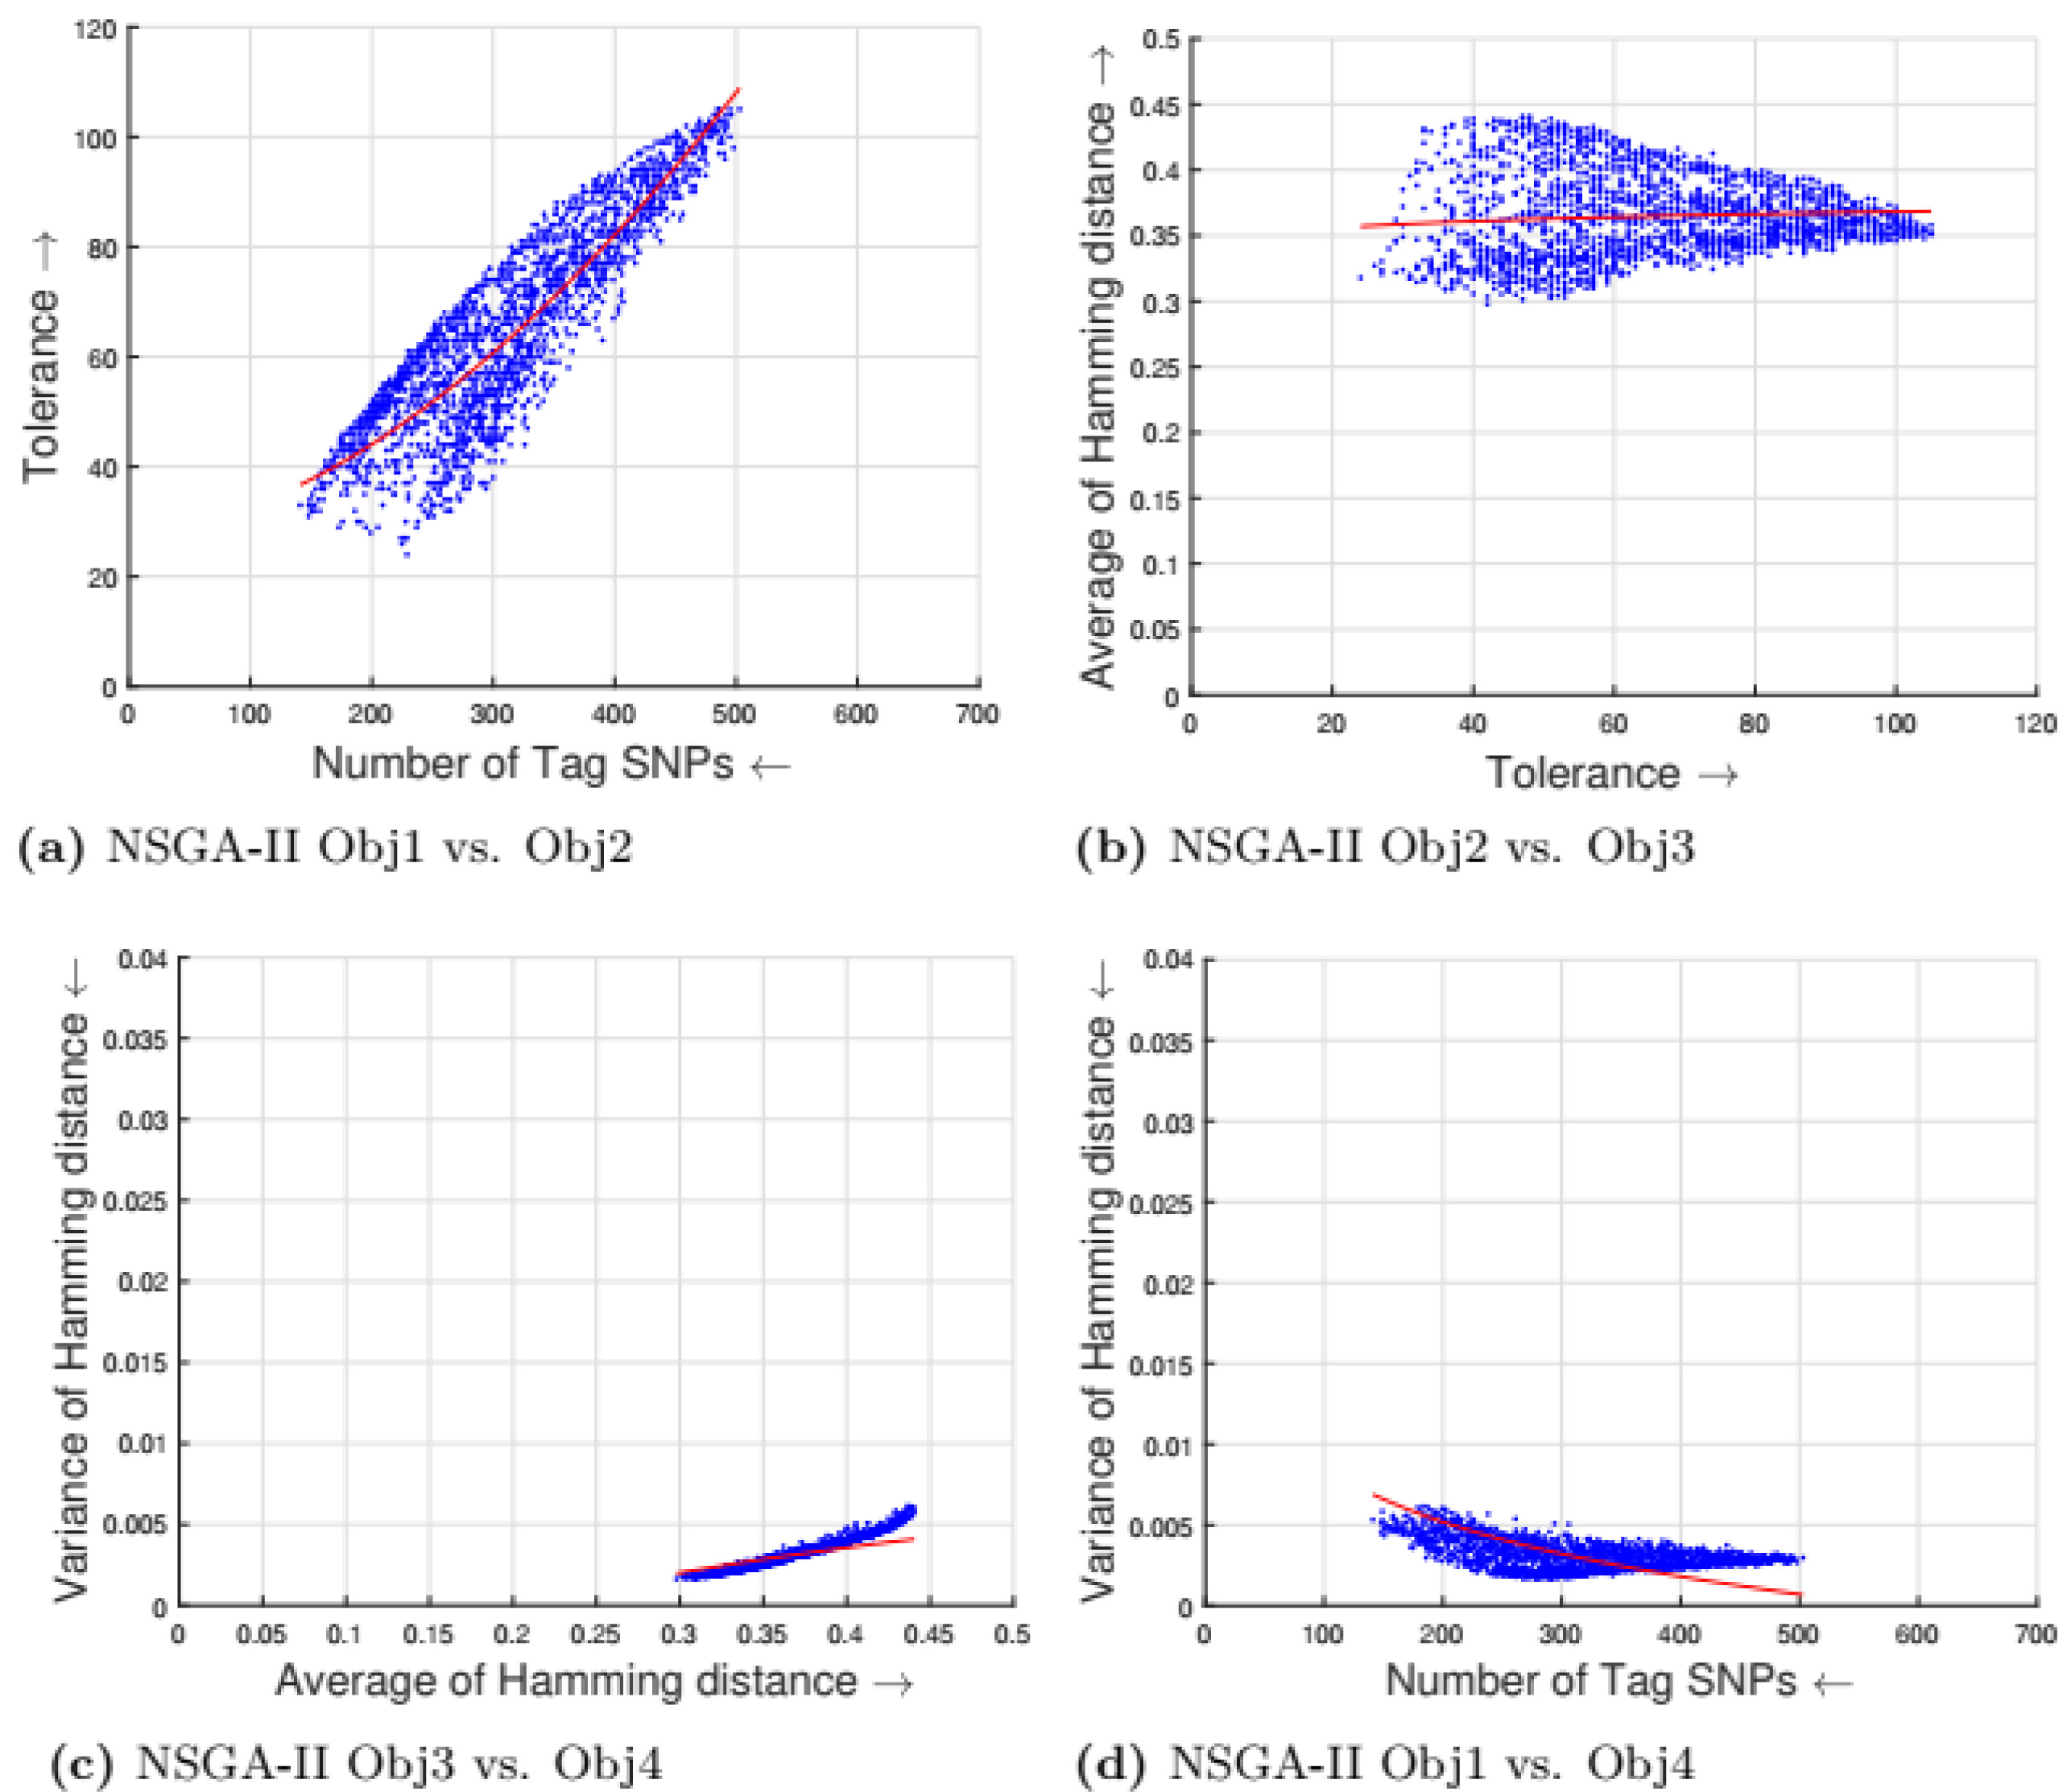
\includegraphics[width=\textwidth]{analisis_assets/moqa_2022/figures/moqa_fig_nsga2_greedy.jpeg}
        \caption{NSGA-II: Greedy (Moqa)}
    \end{subfigure}
    \begin{subfigure}[b]{0.32\textwidth}
        \centering
        
\includegraphics[width=\textwidth]{analisis_assets/20260425T180636/2_comparativa/1_frentes/frentes_pareto/frentes_pareto_nsga2_greedy_hybrid_full.png}
        \caption{NSGA-II: GH (Exp. A)}
    \end{subfigure}
    \begin{subfigure}[b]{0.32\textwidth}
        \centering
        
\includegraphics[width=\textwidth]{analisis_assets/20260425T170417/2_comparativa/1_frentes/frentes_pareto/frentes_pareto_nsga2_greedy_hybrid_full.png}
        \caption{NSGA-II: GH (Exp. B)}
    \end{subfigure}

    \vspace{0.3cm}

    \begin{subfigure}[b]{0.32\textwidth}
        \centering
        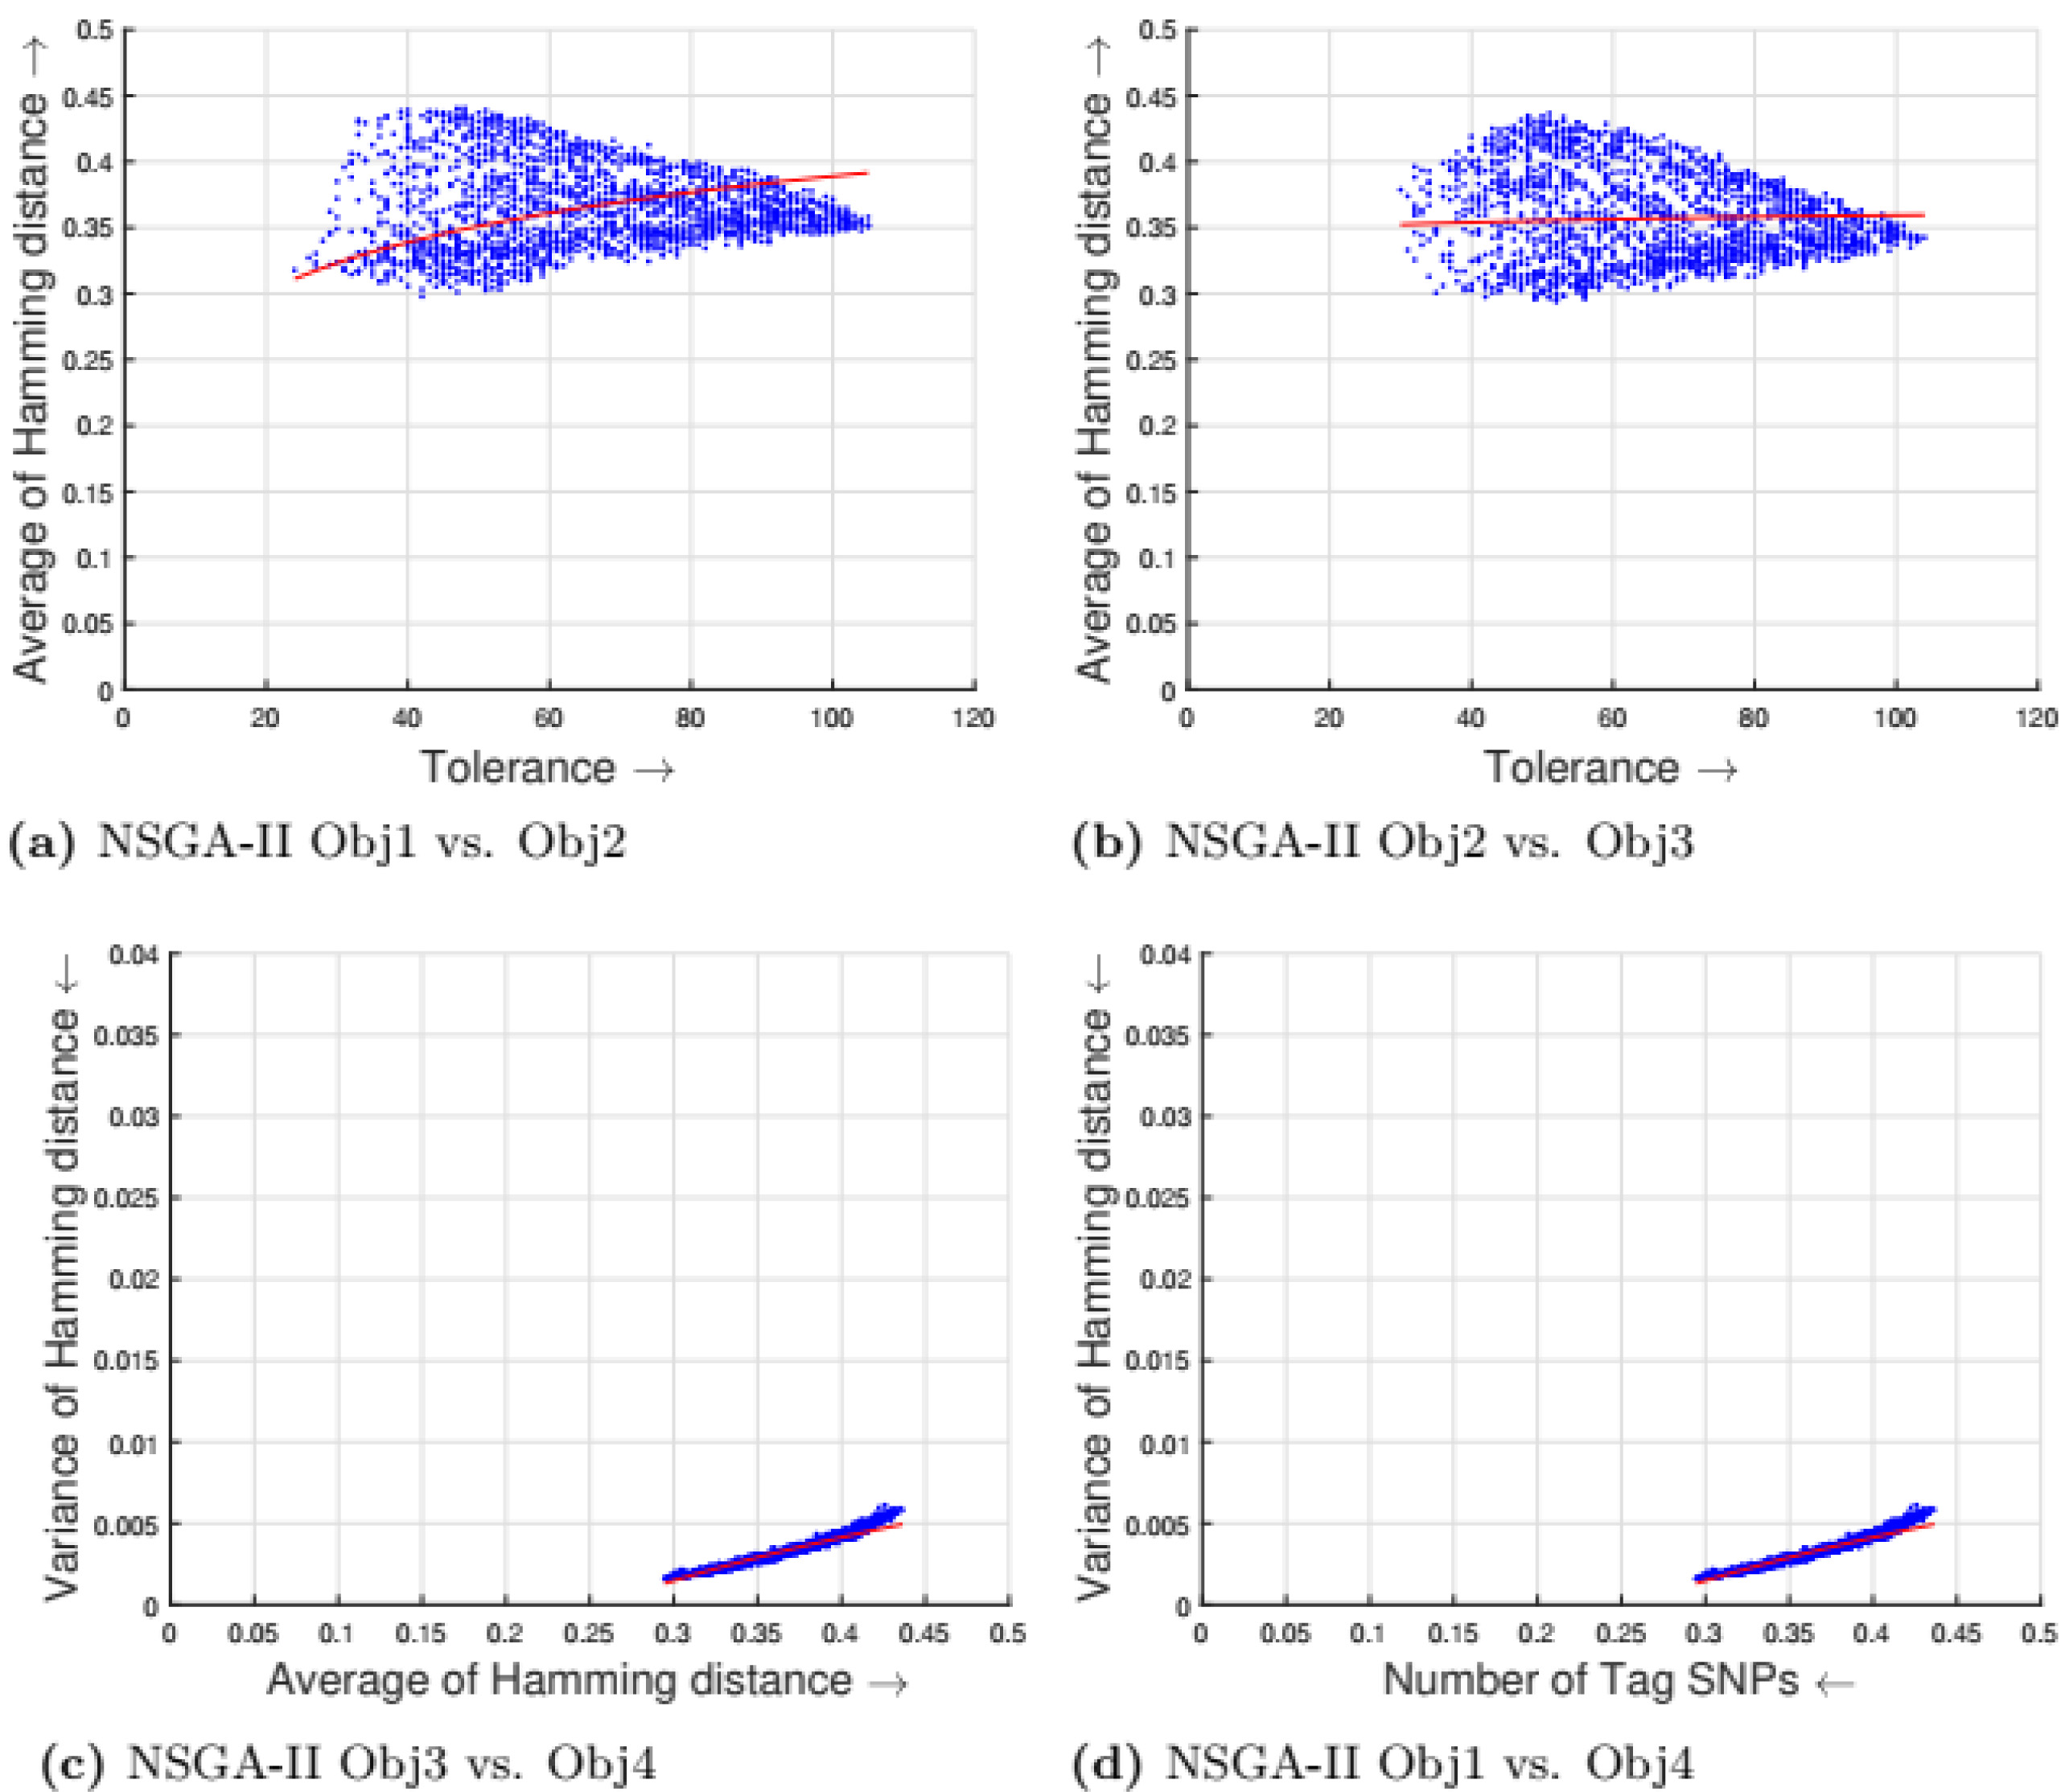
\includegraphics[width=\textwidth]{analisis_assets/moqa_2022/figures/moqa_fig_nsga2_random.jpeg}
        \caption{NSGA-II: Random (Moqa)}
    \end{subfigure}
    \begin{subfigure}[b]{0.32\textwidth}
        \centering
        
\includegraphics[width=\textwidth]{analisis_assets/20260425T180636/2_comparativa/1_frentes/frentes_pareto/frentes_pareto_nsga2_random_dense_full.png}
        \caption{NSGA-II: RD (Exp. A)}
    \end{subfigure}
    \begin{subfigure}[b]{0.32\textwidth}
        \centering
        
\includegraphics[width=\textwidth]{analisis_assets/20260425T170417/2_comparativa/1_frentes/frentes_pareto/frentes_pareto_nsga2_random_dense_full.png}
        \caption{NSGA-II: RD (Exp. B)}
    \end{subfigure}
    \caption{Comparativa de frentes para NSGA-II frente al original de Moqa (Greedy y Random).}
\end{figure}

\subsubsection{Comparativa Algoritmo SPEA2}

\begin{figure}[H]
    \centering
    \begin{subfigure}[b]{0.32\textwidth}
        \centering
        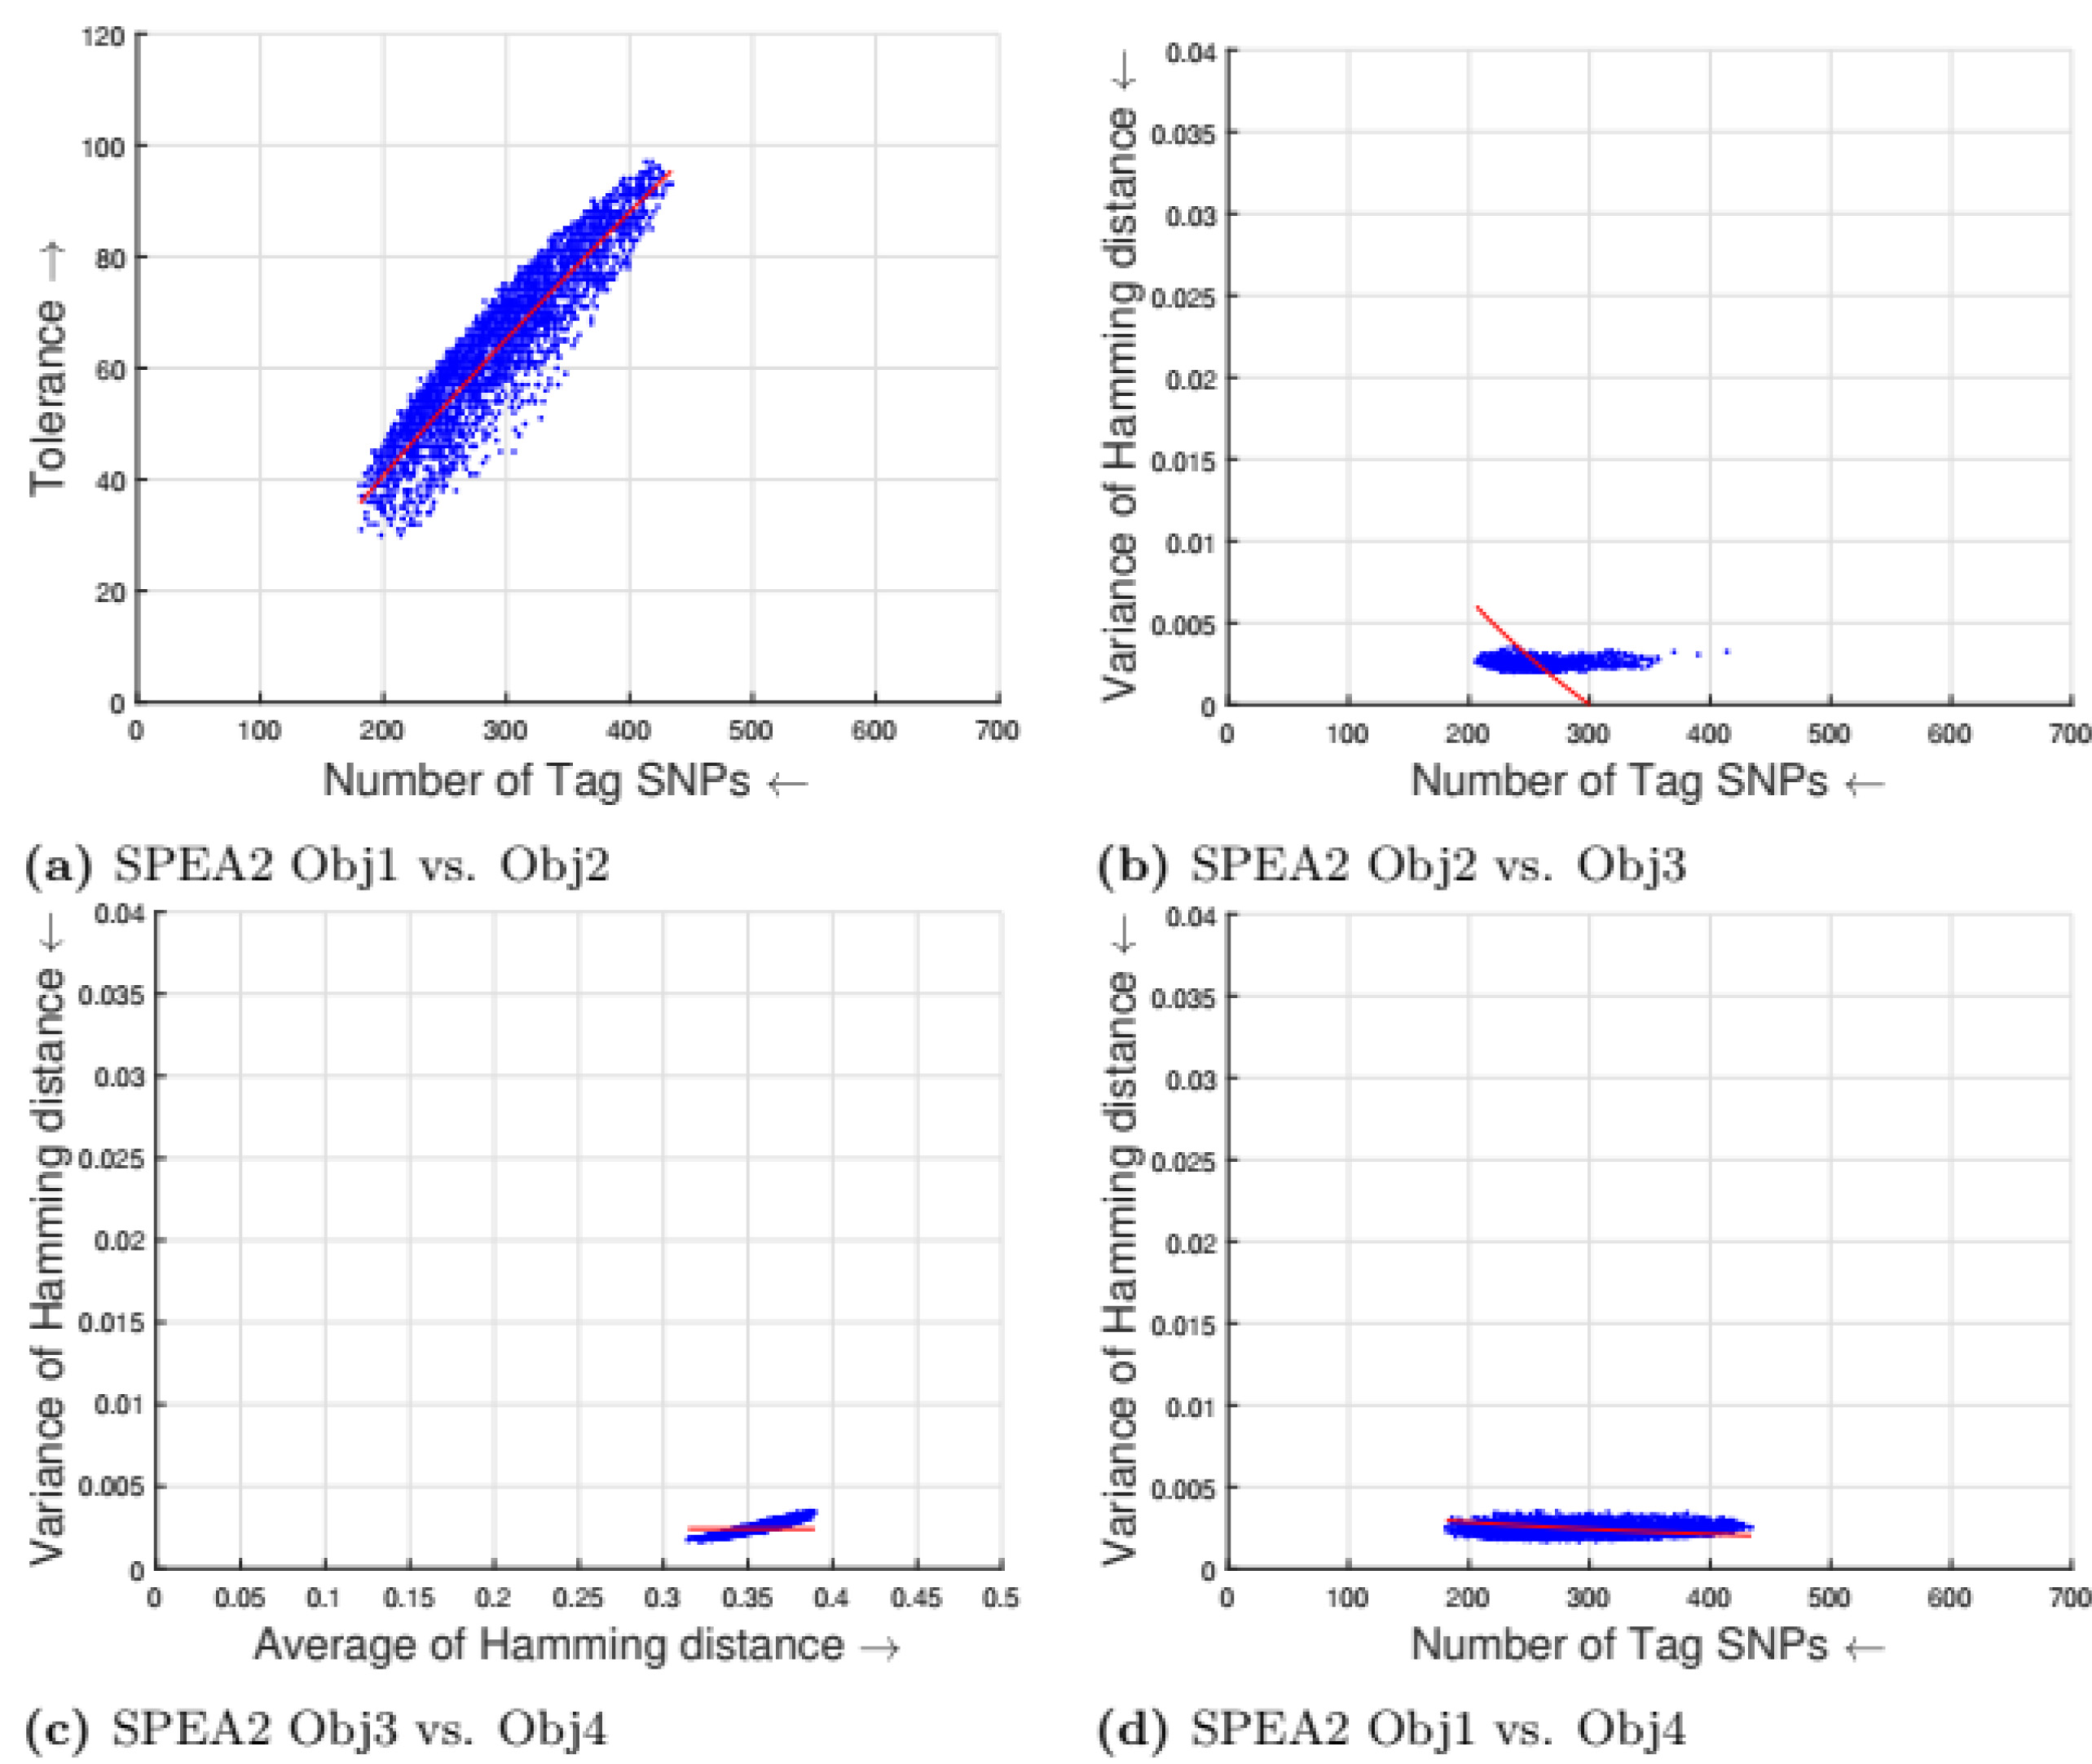
\includegraphics[width=\textwidth]{analisis_assets/moqa_2022/figures/moqa_fig_spea2_greedy.jpeg}
        \caption{SPEA2: Greedy (Moqa)}
    \end{subfigure}
    \begin{subfigure}[b]{0.32\textwidth}
        \centering
        
\includegraphics[width=\textwidth]{analisis_assets/20260425T180636/2_comparativa/1_frentes/frentes_pareto/frentes_pareto_spea2_greedy_hybrid_full.png}
        \caption{SPEA2: GH (Exp. A)}
    \end{subfigure}
    \begin{subfigure}[b]{0.32\textwidth}
        \centering
        
\includegraphics[width=\textwidth]{analisis_assets/20260425T170417/2_comparativa/1_frentes/frentes_pareto/frentes_pareto_spea2_greedy_hybrid_full.png}
        \caption{SPEA2: GH (Exp. B)}
    \end{subfigure}

    \vspace{0.3cm}

    \begin{subfigure}[b]{0.32\textwidth}
        \centering
        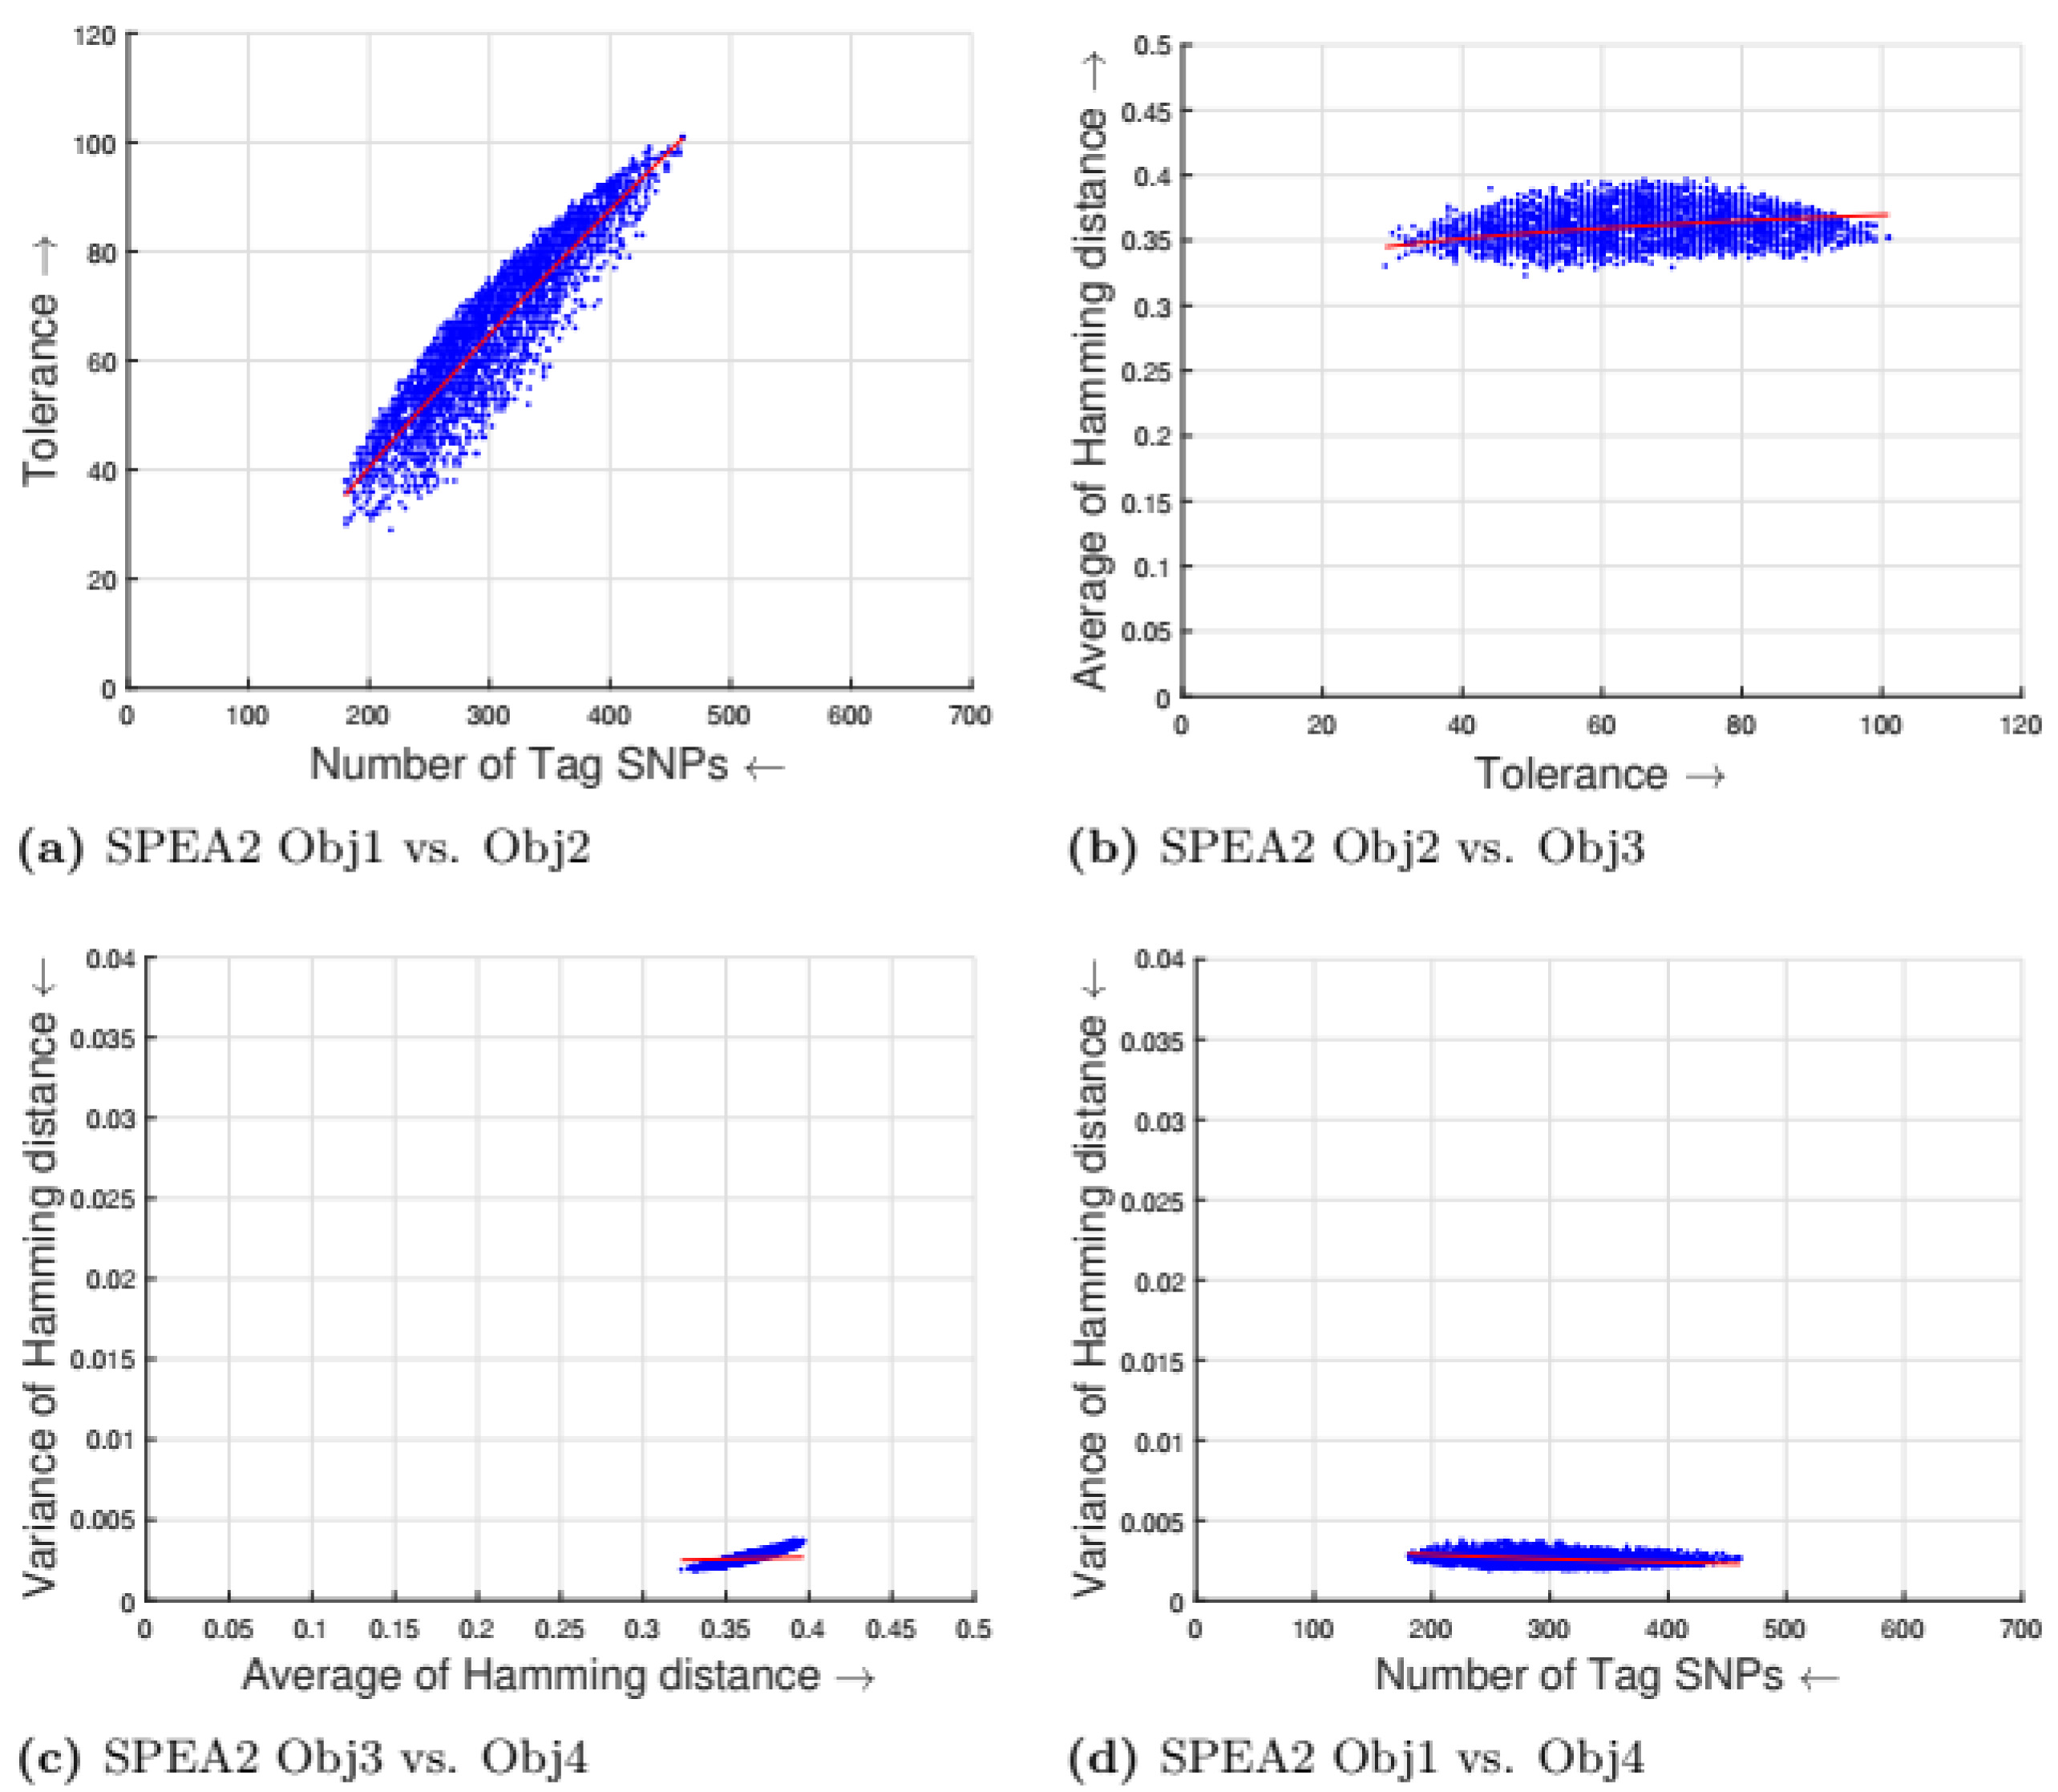
\includegraphics[width=\textwidth]{analisis_assets/moqa_2022/figures/moqa_fig_spea2_random.jpeg}
        \caption{SPEA2: Random (Moqa)}
    \end{subfigure}
    \begin{subfigure}[b]{0.32\textwidth}
        \centering
        
\includegraphics[width=\textwidth]{analisis_assets/20260425T180636/2_comparativa/1_frentes/frentes_pareto/frentes_pareto_spea2_random_dense_full.png}
        \caption{SPEA2: RD (Exp. A)}
    \end{subfigure}
    \begin{subfigure}[b]{0.32\textwidth}
        \centering
        
\includegraphics[width=\textwidth]{analisis_assets/20260425T170417/2_comparativa/1_frentes/frentes_pareto/frentes_pareto_spea2_random_dense_full.png}
        \caption{SPEA2: RD (Exp. B)}
    \end{subfigure}
    \caption{Comparativa de frentes para SPEA2 frente al original de Moqa (Greedy y Random).}
\end{figure}

\subsubsection{Comparativa Algoritmo NSGA-III}

\begin{figure}[H]
    \centering
    \begin{subfigure}[b]{0.32\textwidth}
        \centering
        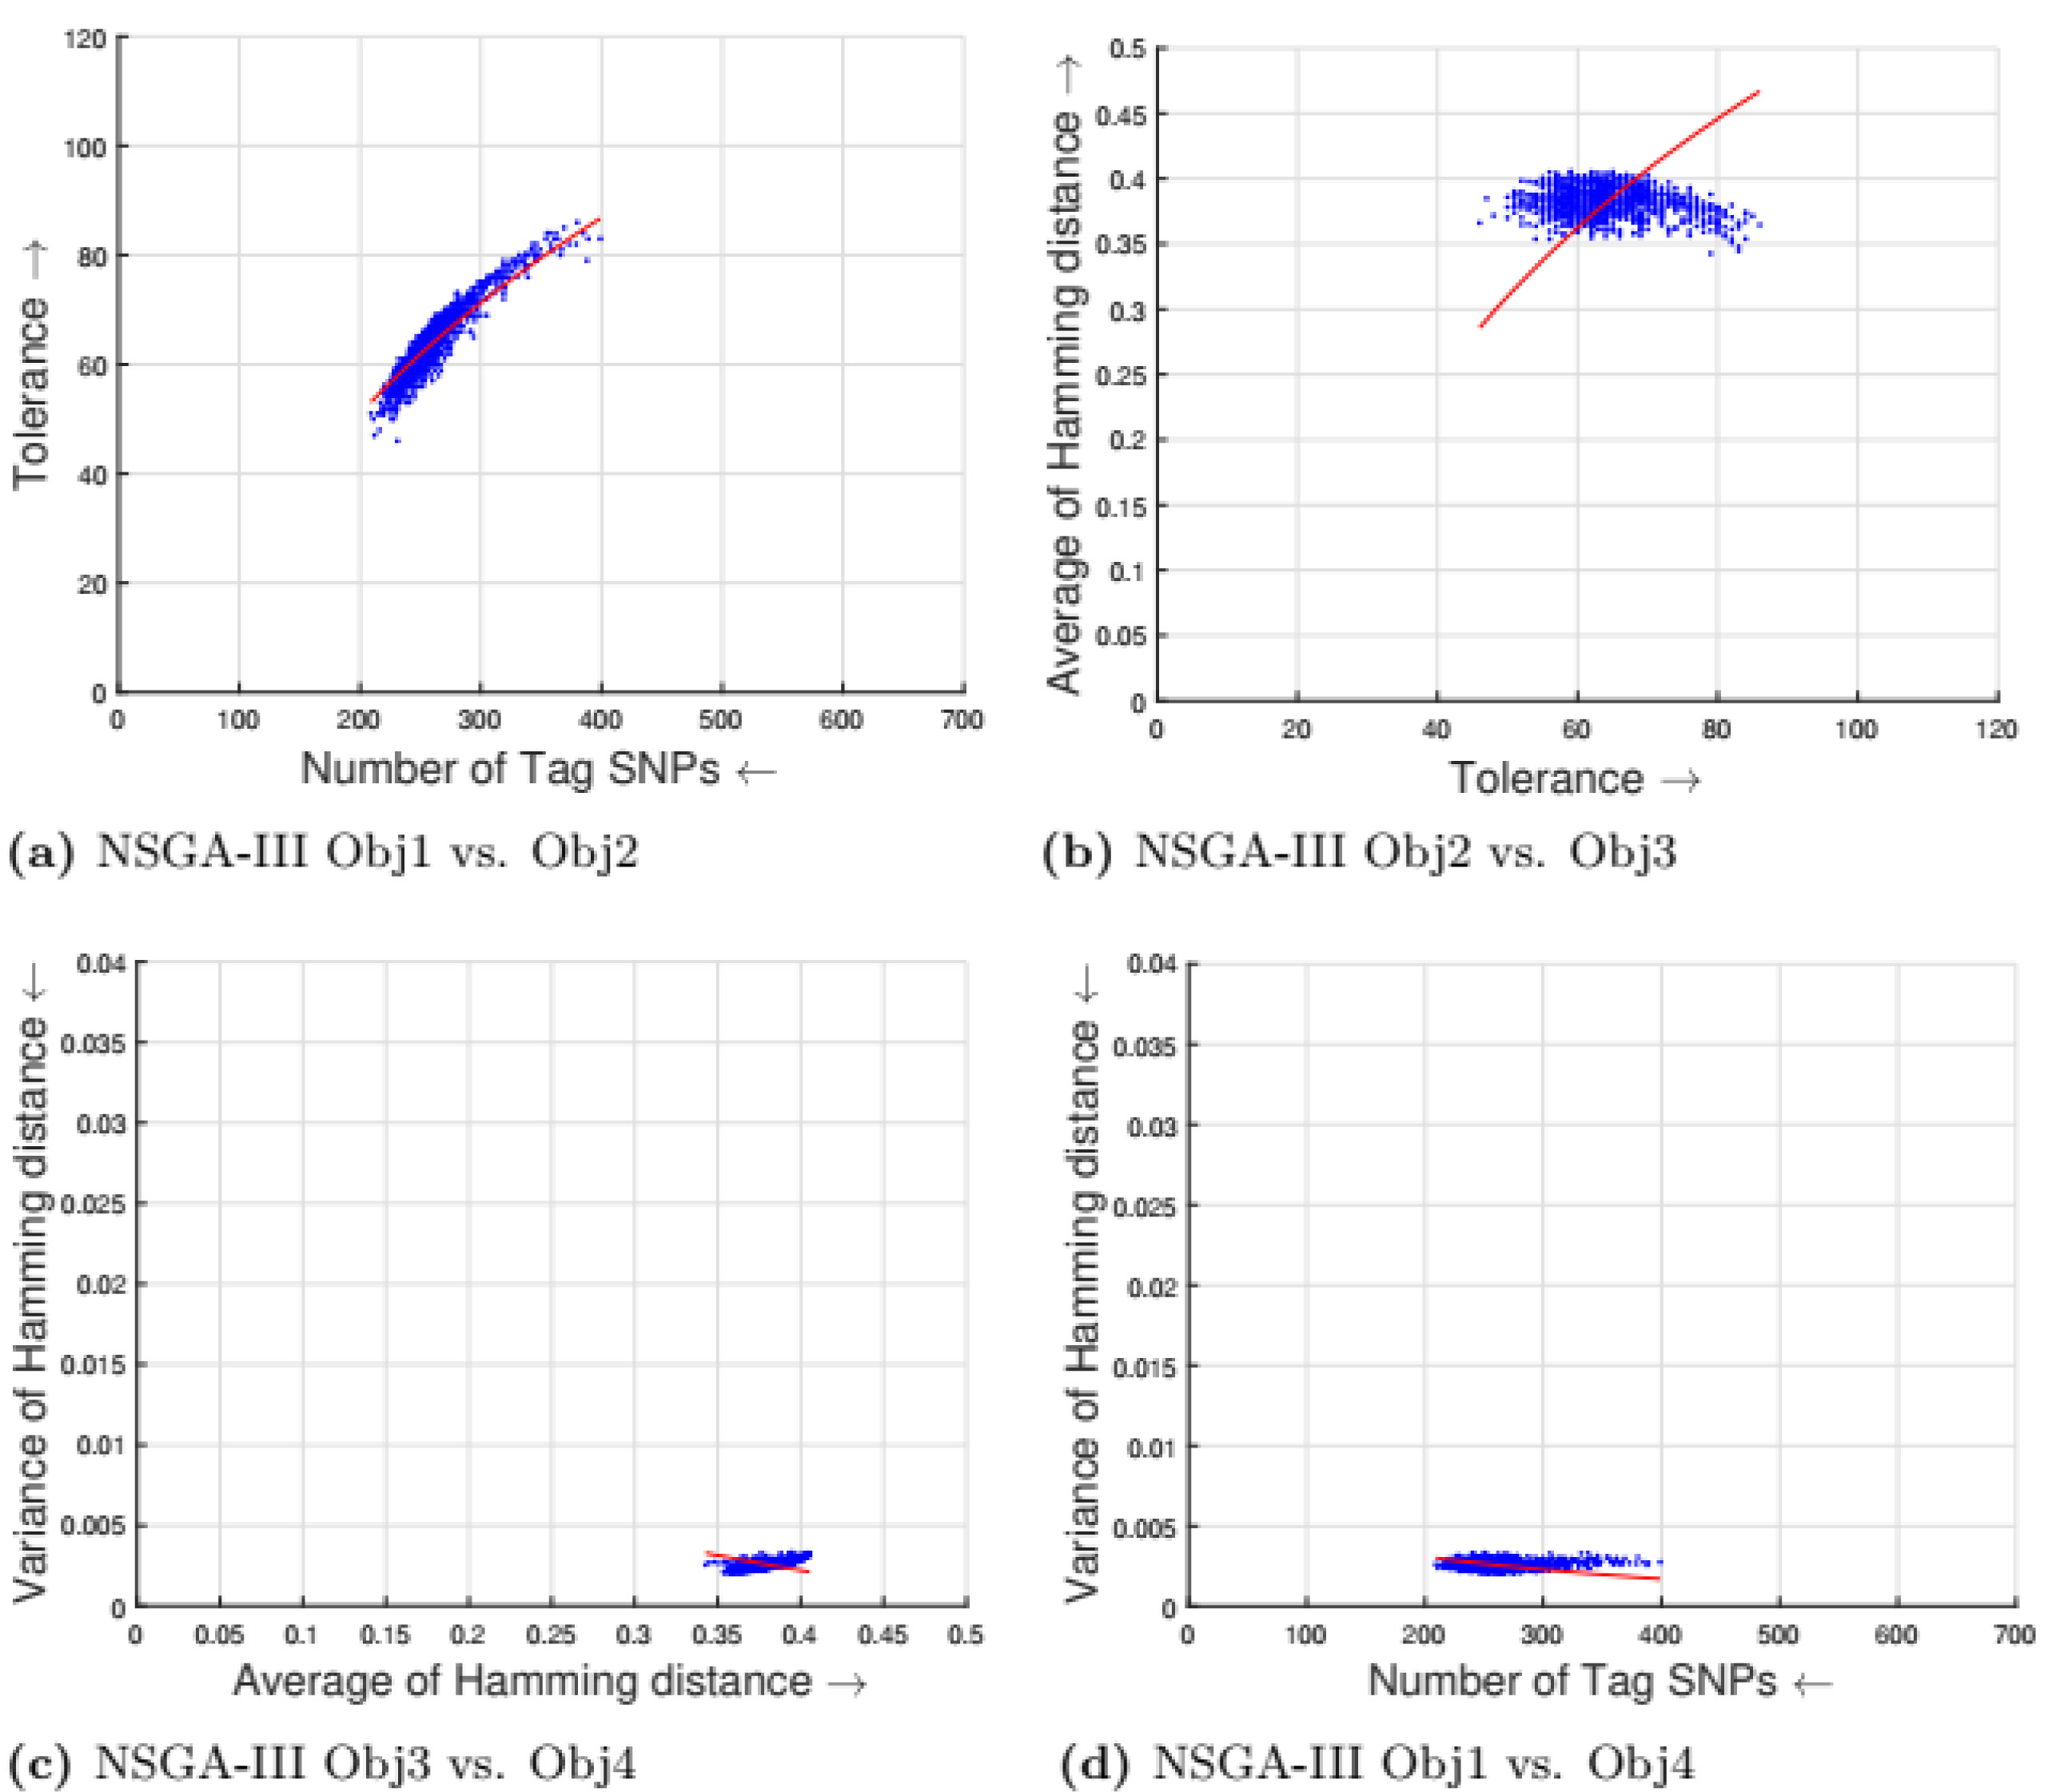
\includegraphics[width=\textwidth]{analisis_assets/moqa_2022/figures/moqa_fig_nsga3_greedy.jpeg}
        \caption{NSGA-III: Greedy (Moqa)}
    \end{subfigure}
    \begin{subfigure}[b]{0.32\textwidth}
        \centering
        
\includegraphics[width=\textwidth]{analisis_assets/20260425T180636/2_comparativa/1_frentes/frentes_pareto/frentes_pareto_nsga3_greedy_hybrid_full.png}
        \caption{NSGA-III: GH (Exp. A)}
    \end{subfigure}
    \begin{subfigure}[b]{0.32\textwidth}
        \centering
        
\includegraphics[width=\textwidth]{analisis_assets/20260425T170417/2_comparativa/1_frentes/frentes_pareto/frentes_pareto_nsga3_greedy_hybrid_full.png}
        \caption{NSGA-III: GH (Exp. B)}
    \end{subfigure}

    \vspace{0.3cm}

    \begin{subfigure}[b]{0.32\textwidth}
        \centering
        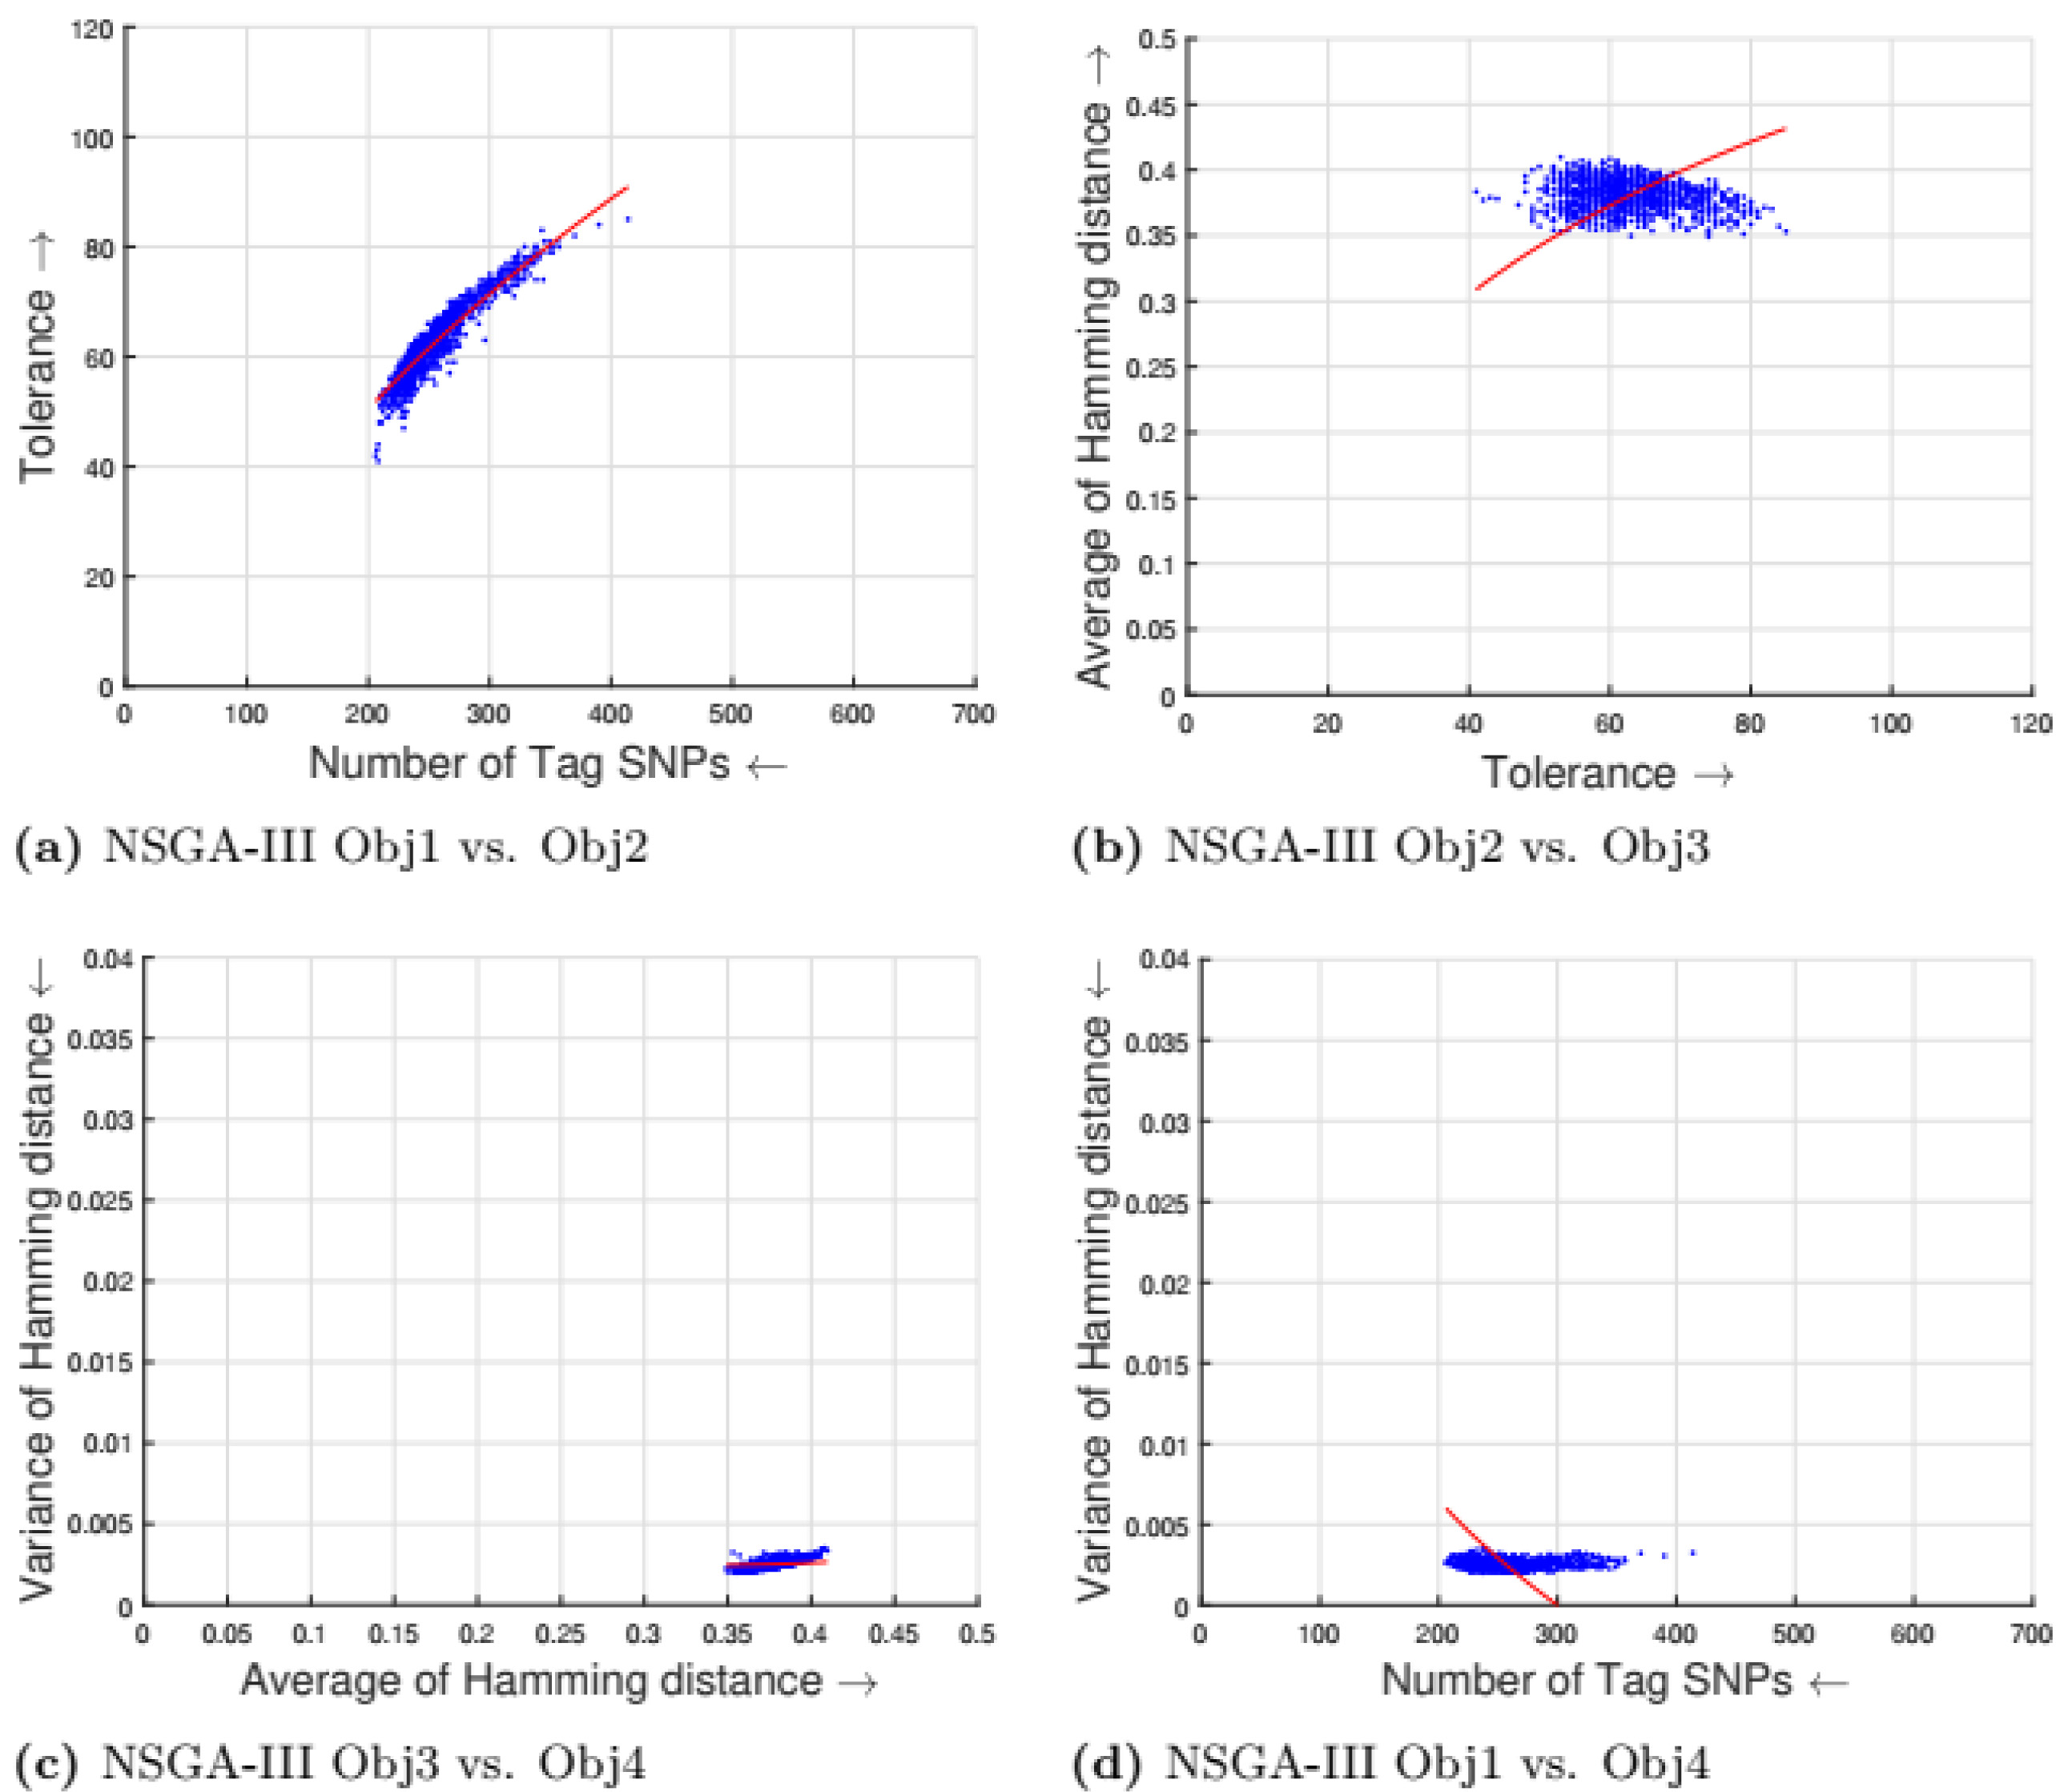
\includegraphics[width=\textwidth]{analisis_assets/moqa_2022/figures/moqa_fig_nsga3_random.jpeg}
        \caption{NSGA-III: Random (Moqa)}
    \end{subfigure}
    \begin{subfigure}[b]{0.32\textwidth}
        \centering
        
\includegraphics[width=\textwidth]{analisis_assets/20260425T180636/2_comparativa/1_frentes/frentes_pareto/frentes_pareto_nsga3_random_dense_full.png}
        \caption{NSGA-III: RD (Exp. A)}
    \end{subfigure}
    \begin{subfigure}[b]{0.32\textwidth}
        \centering
        
\includegraphics[width=\textwidth]{analisis_assets/20260425T170417/2_comparativa/1_frentes/frentes_pareto/frentes_pareto_nsga3_random_dense_full.png}
        \caption{NSGA-III: RD (Exp. B)}
    \end{subfigure}
    \caption{Comparativa de frentes para NSGA-III frente al original de Moqa (Greedy y Random).}
\end{figure}

\subsubsection{MOEA/D: Análisis de la variante PBI}

\begin{figure}[H]
    \centering
    \begin{subfigure}[b]{0.32\textwidth}
        \centering
        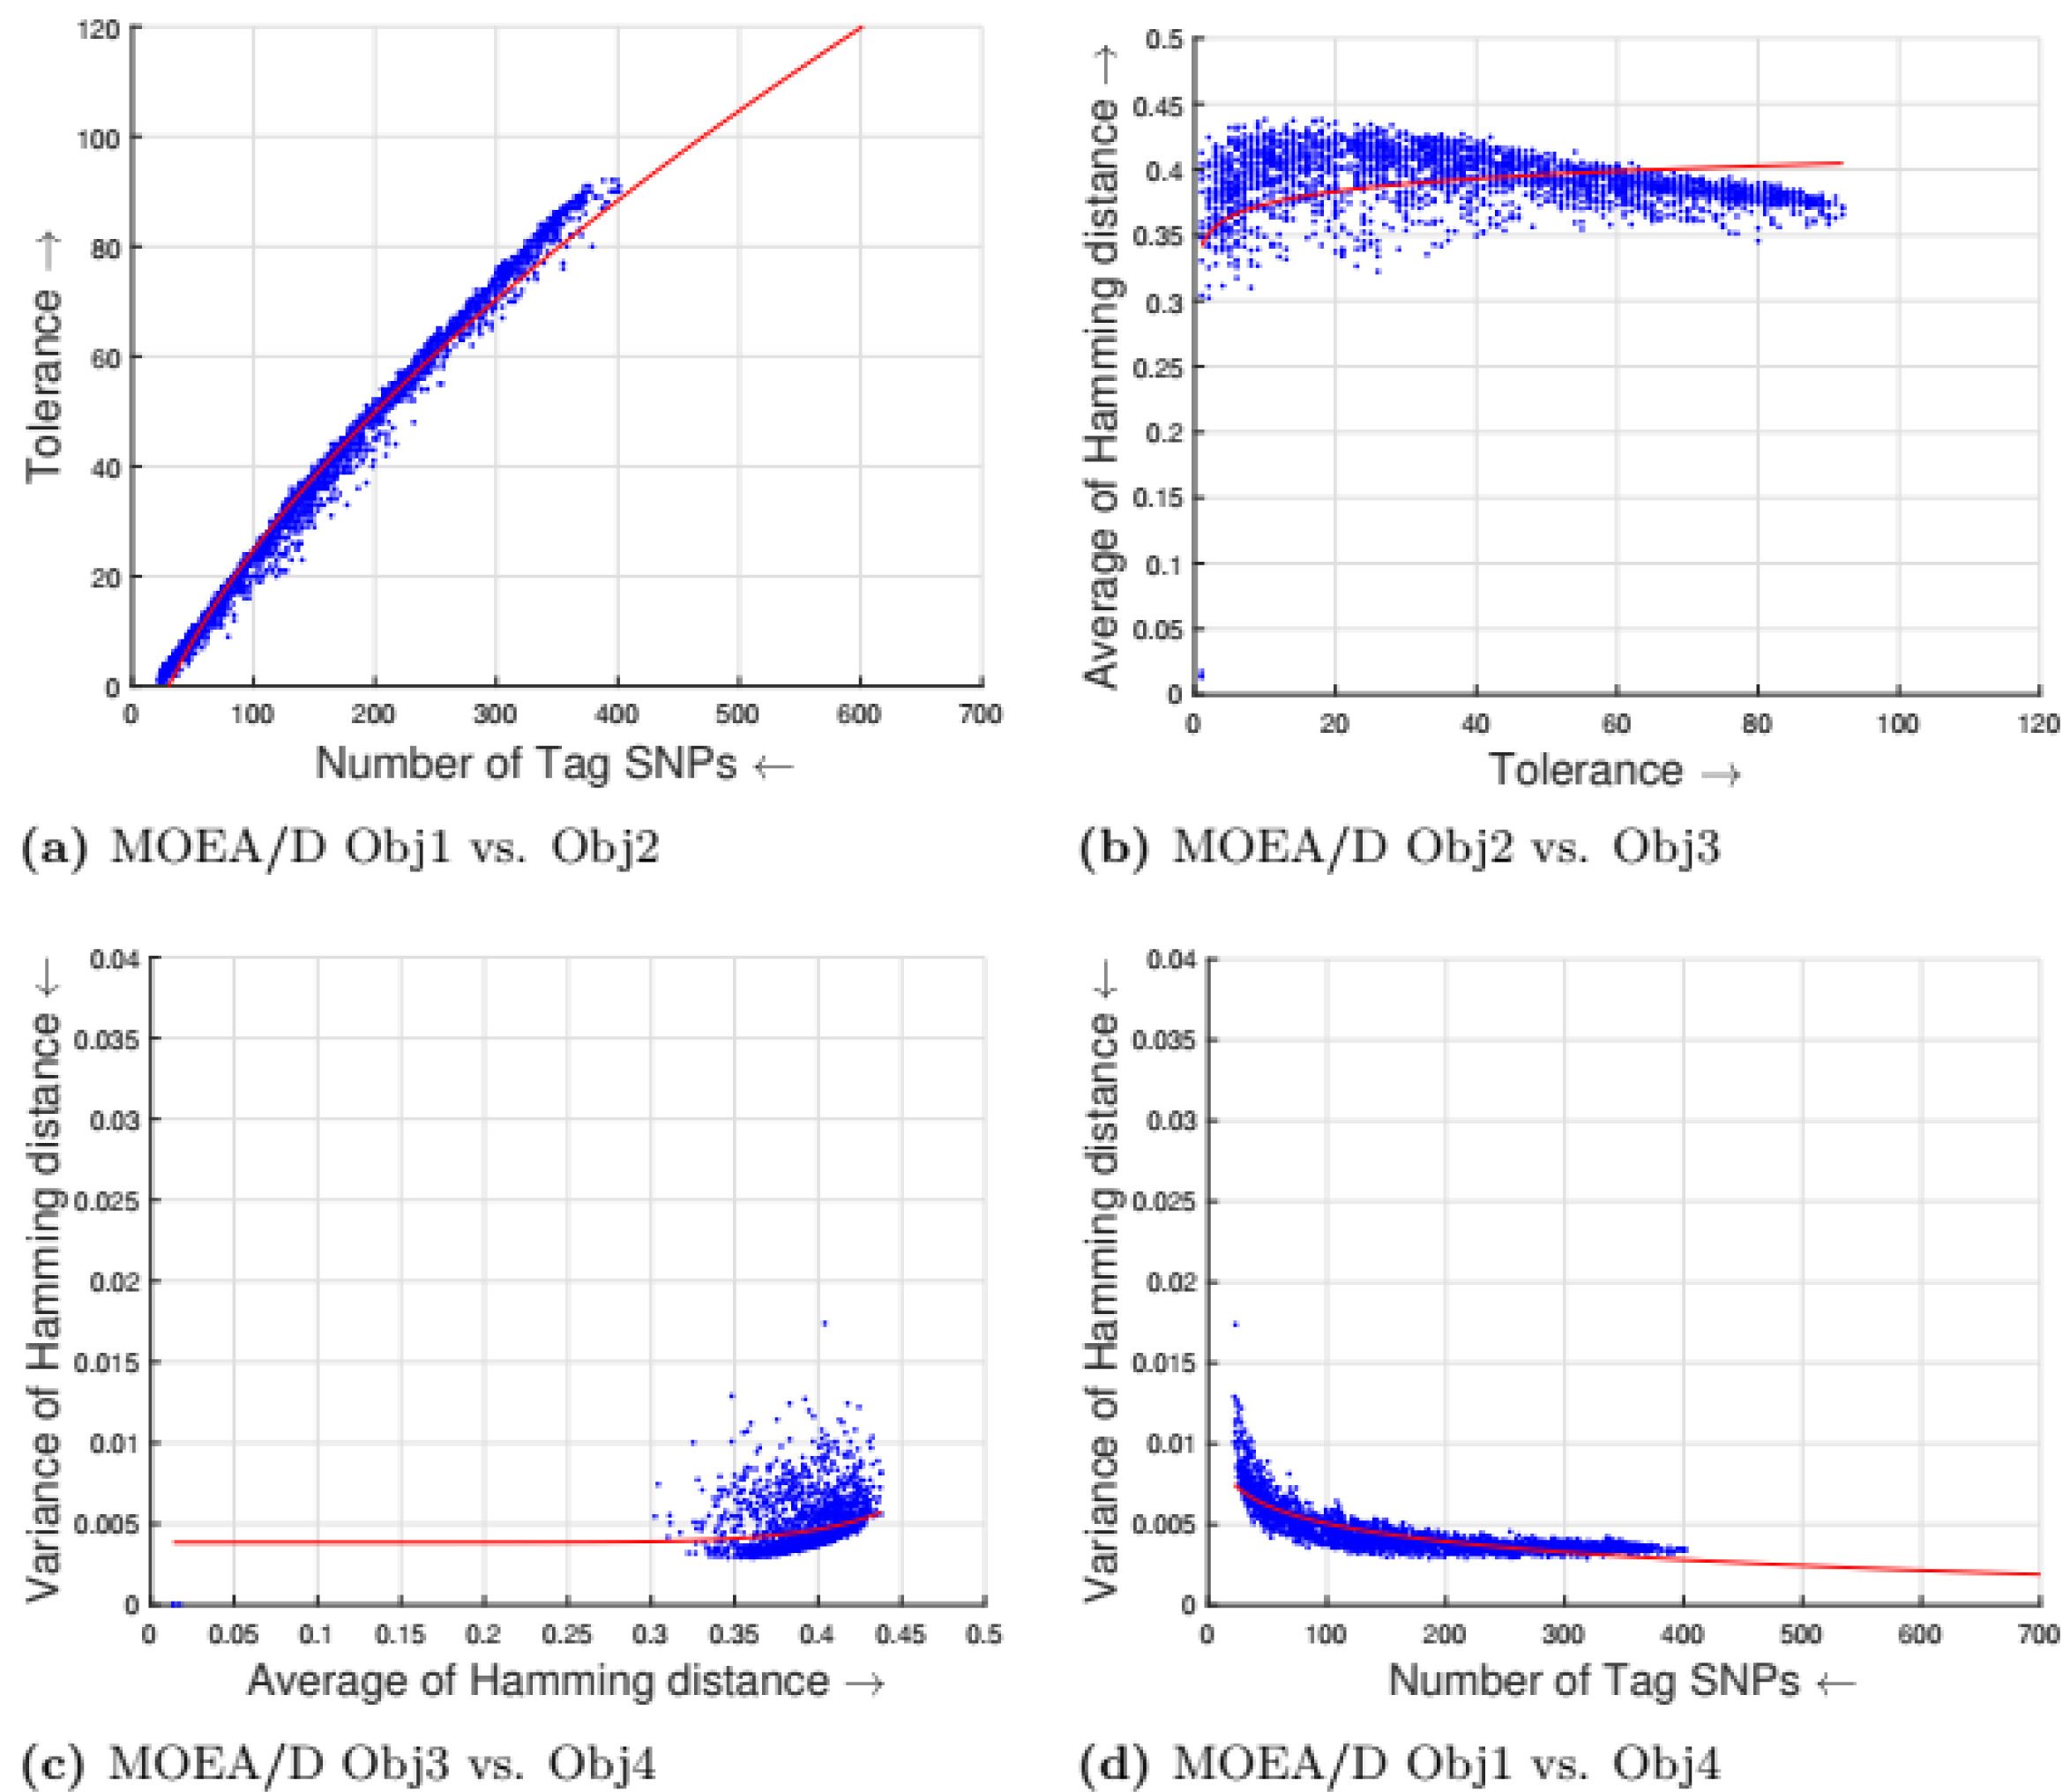
\includegraphics[width=\textwidth]{analisis_assets/moqa_2022/figures/moqa_fig_moead_greedy.jpeg}
        \caption{MOEA/D: Greedy (Moqa)}
    \end{subfigure}
    \begin{subfigure}[b]{0.32\textwidth}
        \centering
        
\includegraphics[width=\textwidth]{analisis_assets/20260425T180636/2_comparativa/1_frentes/frentes_pareto/frentes_pareto_moead_pbi_greedy_hybrid_full.png}
        \caption{PBI: Greedy Hybrid (Exp. A)}
    \end{subfigure}
    \begin{subfigure}[b]{0.32\textwidth}
        \centering
        
\includegraphics[width=\textwidth]{analisis_assets/20260425T170417/2_comparativa/1_frentes/frentes_pareto/frentes_pareto_moead_pbi_greedy_hybrid_full.png}
        \caption{PBI: Greedy Hybrid (Exp. B)}
    \end{subfigure}

    \vspace{0.3cm}

    \begin{subfigure}[b]{0.32\textwidth}
        \centering
        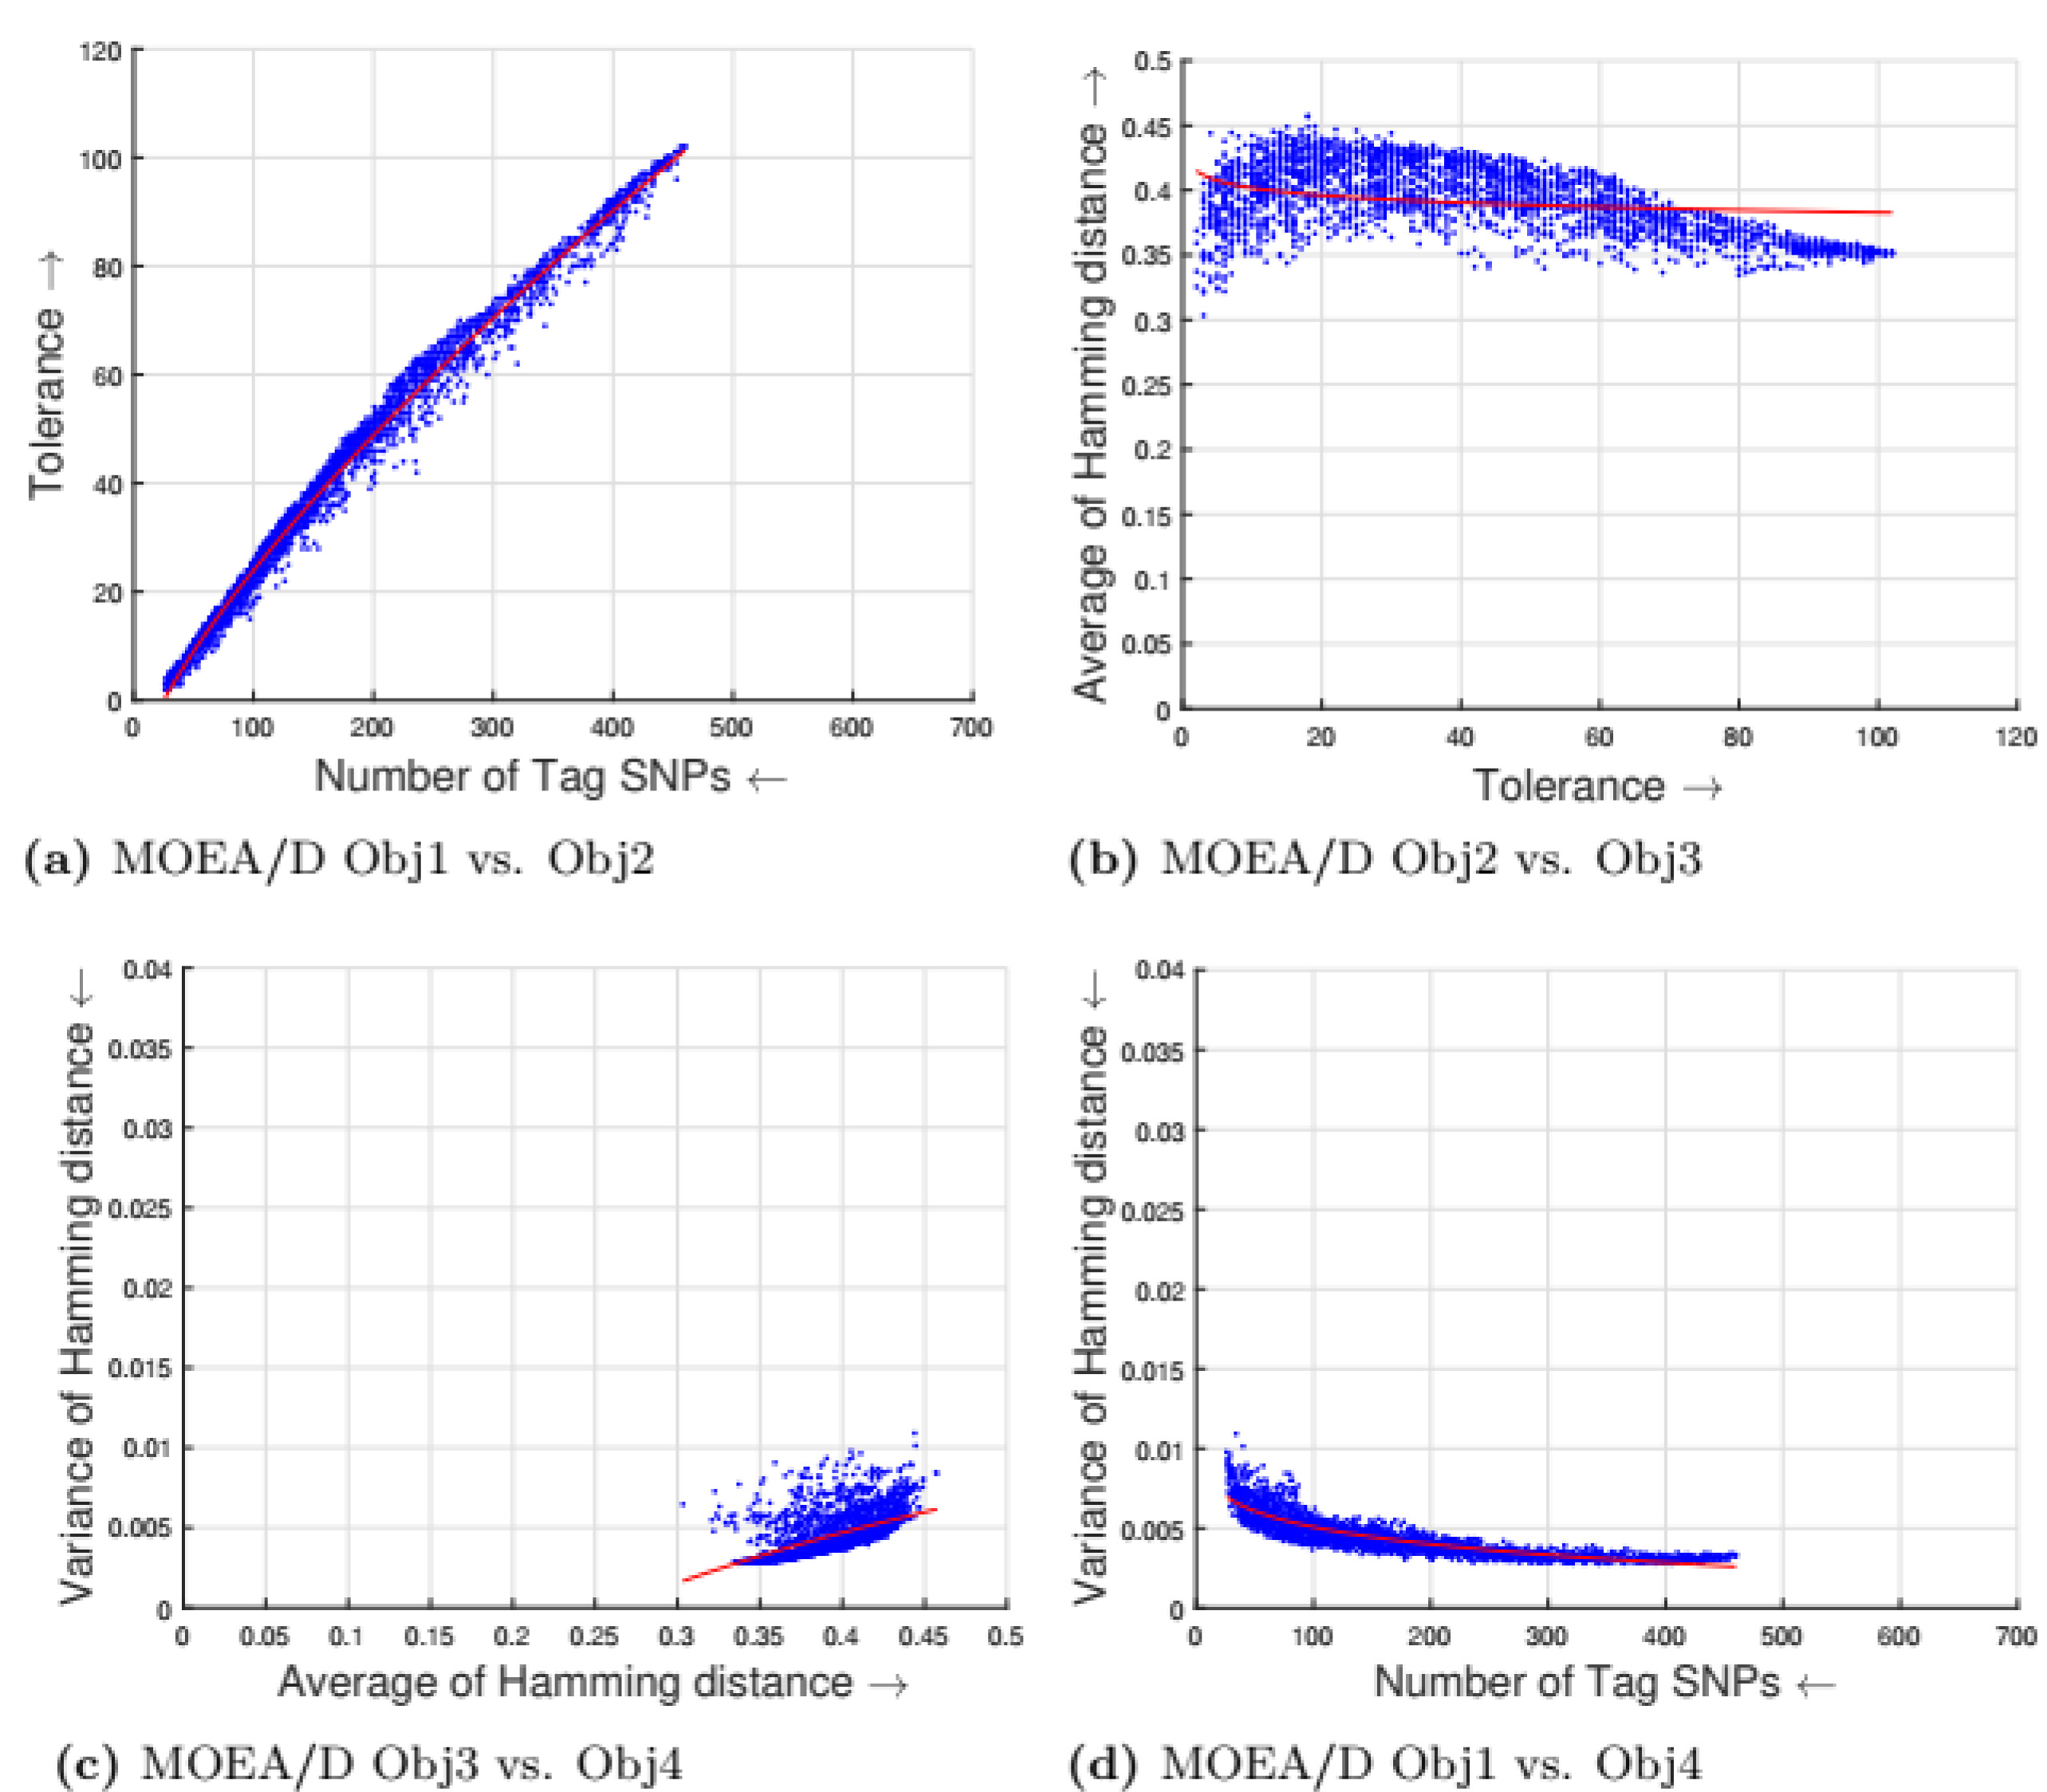
\includegraphics[width=\textwidth]{analisis_assets/moqa_2022/figures/moqa_fig_moead_random.jpeg}
        \caption{MOEA/D: Random (Moqa)}
    \end{subfigure}
    \begin{subfigure}[b]{0.32\textwidth}
        \centering
        
\includegraphics[width=\textwidth]{analisis_assets/20260425T180636/2_comparativa/1_frentes/frentes_pareto/frentes_pareto_moead_pbi_random_dense_full.png}
        \caption{PBI: Random Dense (Exp. A)}
    \end{subfigure}
    \begin{subfigure}[b]{0.32\textwidth}
        \centering
        
\includegraphics[width=\textwidth]{analisis_assets/20260425T170417/2_comparativa/1_frentes/frentes_pareto/frentes_pareto_moead_pbi_random_dense_full.png}
        \caption{PBI: Random Dense (Exp. B)}
    \end{subfigure}
    \caption{Comparativa de frentes para MOEA/D-PBI frente al original de Moqa (Greedy y Random).}
\end{figure}

\subsubsection{MOEA/D: Análisis de la variante Tchebycheff (TCHE)}

\begin{figure}[H]
    \centering
    \begin{subfigure}[b]{0.32\textwidth}
        \centering
        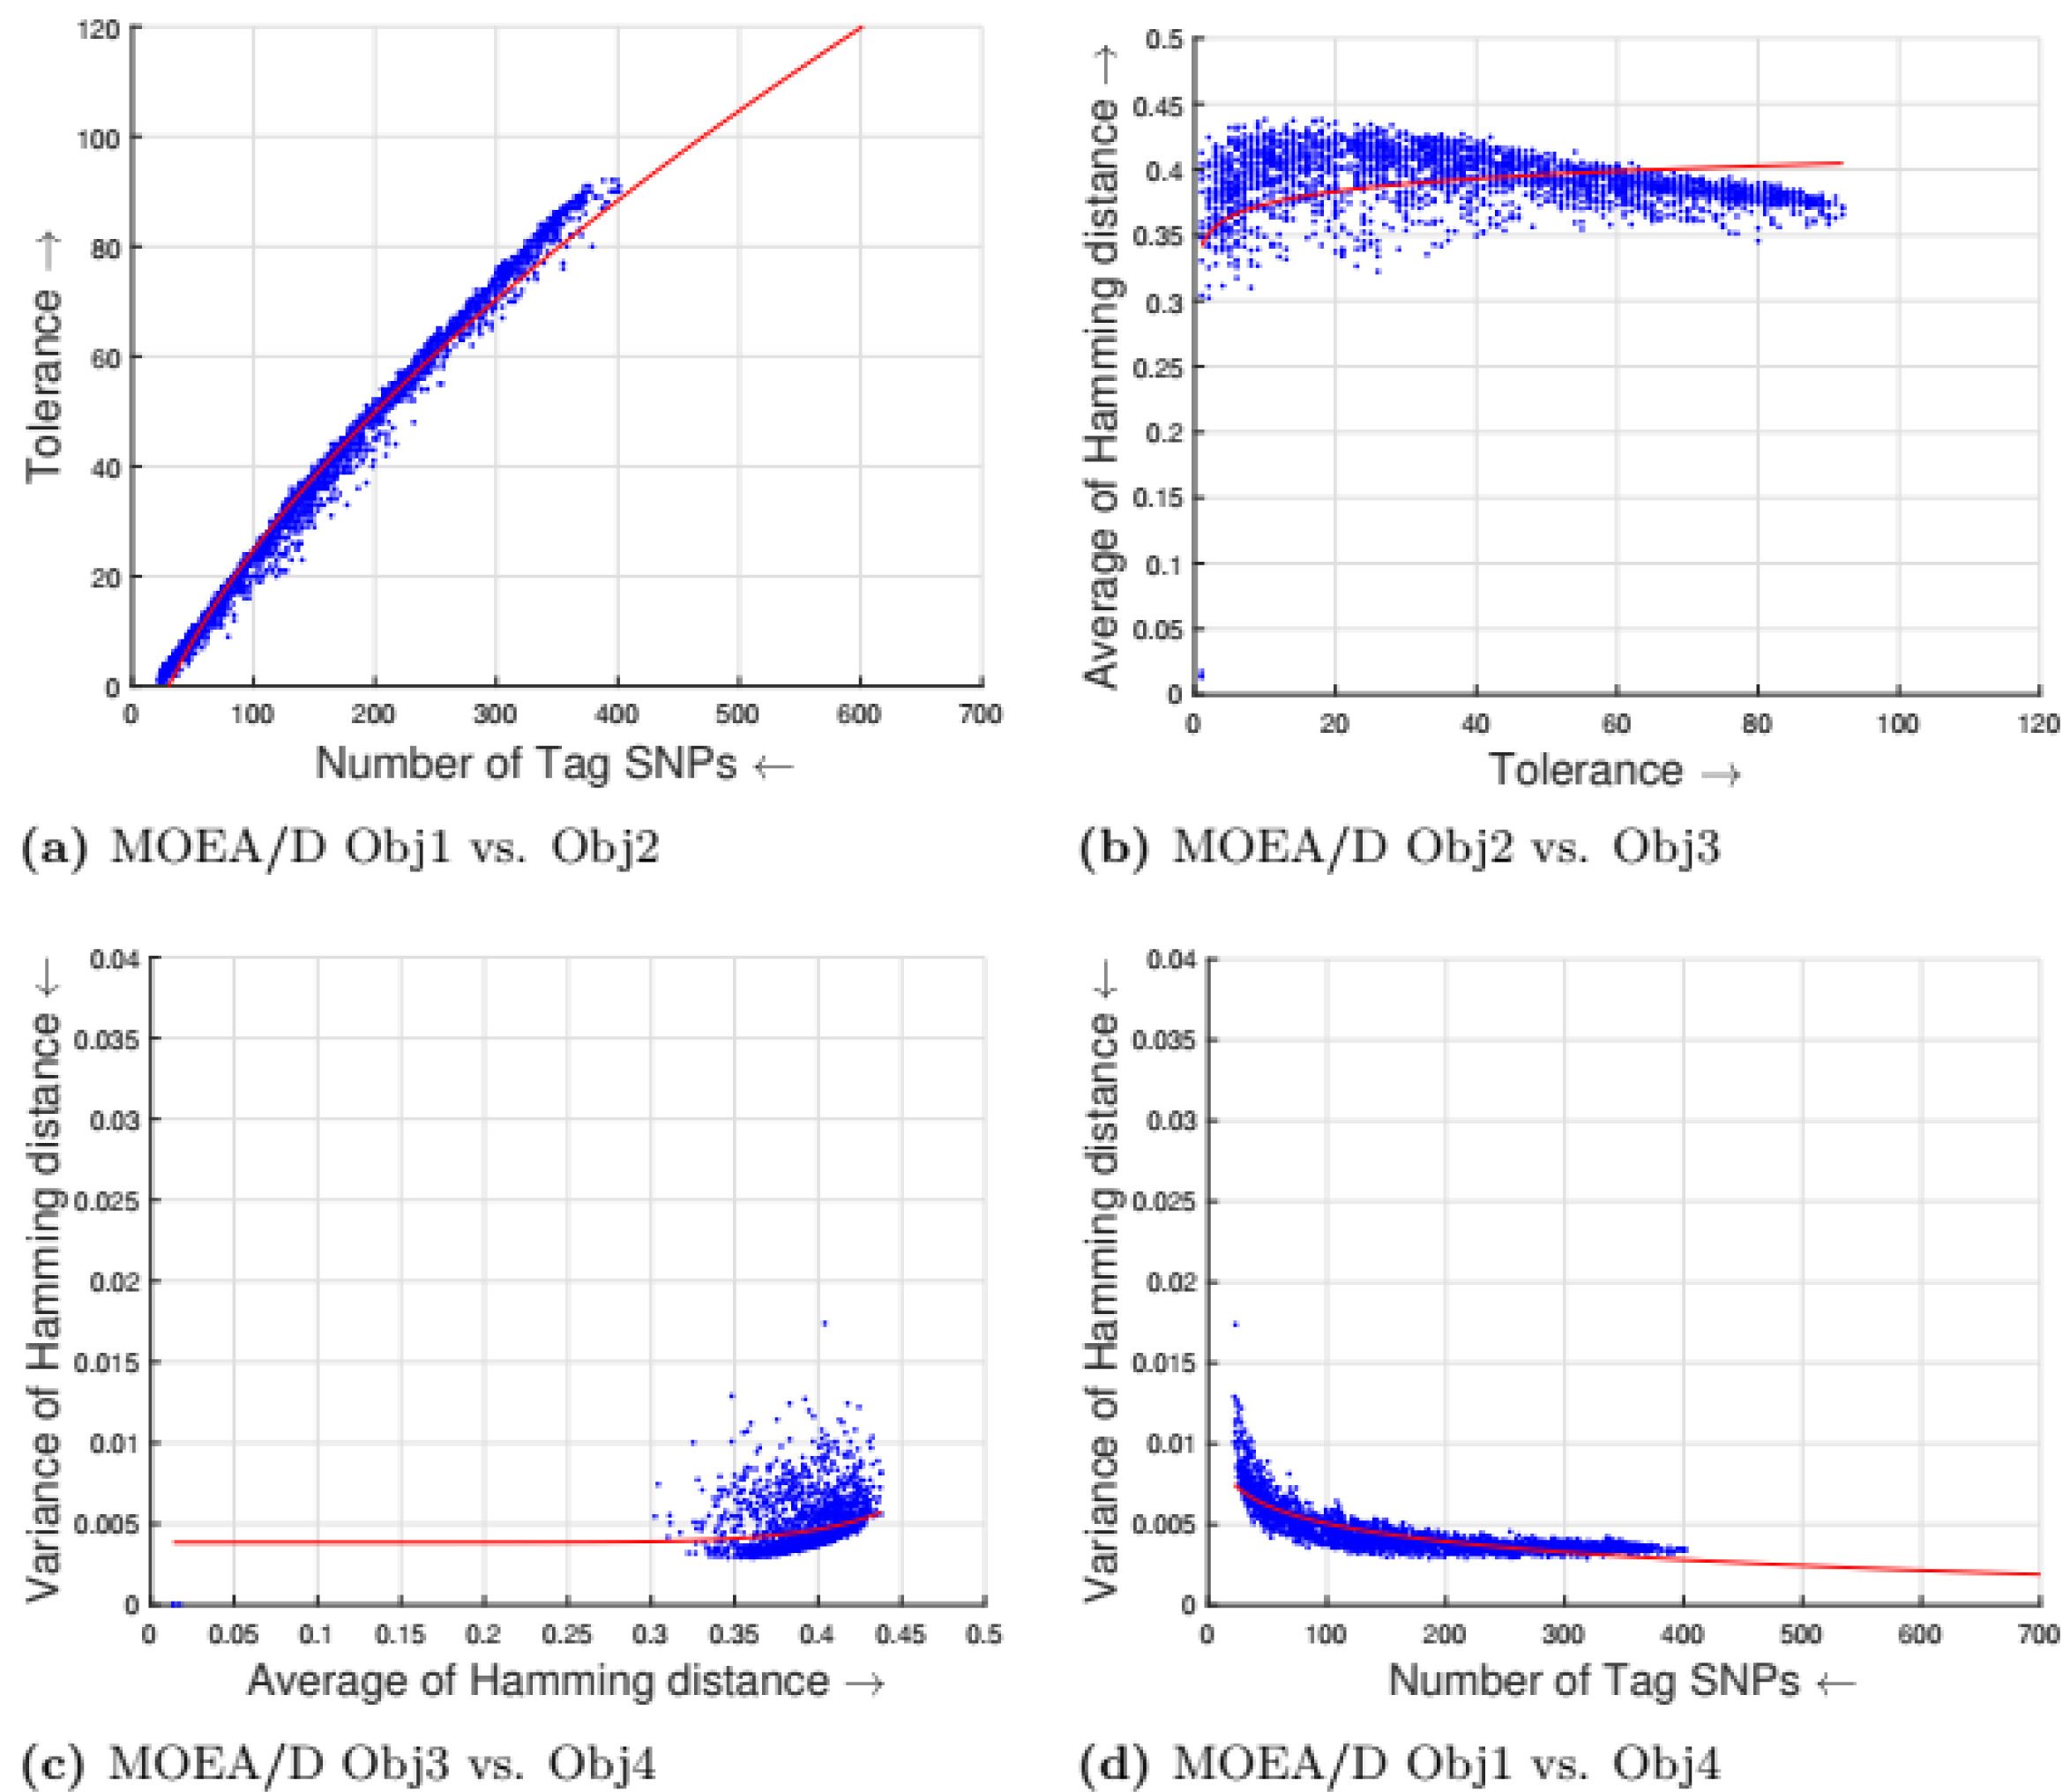
\includegraphics[width=\textwidth]{analisis_assets/moqa_2022/figures/moqa_fig_moead_greedy.jpeg}
        \caption{MOEA/D: Greedy (Moqa)}
    \end{subfigure}
    \begin{subfigure}[b]{0.32\textwidth}
        \centering
        
\includegraphics[width=\textwidth]{analisis_assets/20260425T180636/2_comparativa/1_frentes/frentes_pareto/frentes_pareto_moead_tche_greedy_hybrid_full.png}
        \caption{TCHE: Greedy Hybrid (Exp. A)}
    \end{subfigure}
    \begin{subfigure}[b]{0.32\textwidth}
        \centering
        
\includegraphics[width=\textwidth]{analisis_assets/20260425T170417/2_comparativa/1_frentes/frentes_pareto/frentes_pareto_moead_tche_greedy_hybrid_full.png}
        \caption{TCHE: Greedy Hybrid (Exp. B)}
    \end{subfigure}

    \vspace{0.3cm}

    \begin{subfigure}[b]{0.32\textwidth}
        \centering
        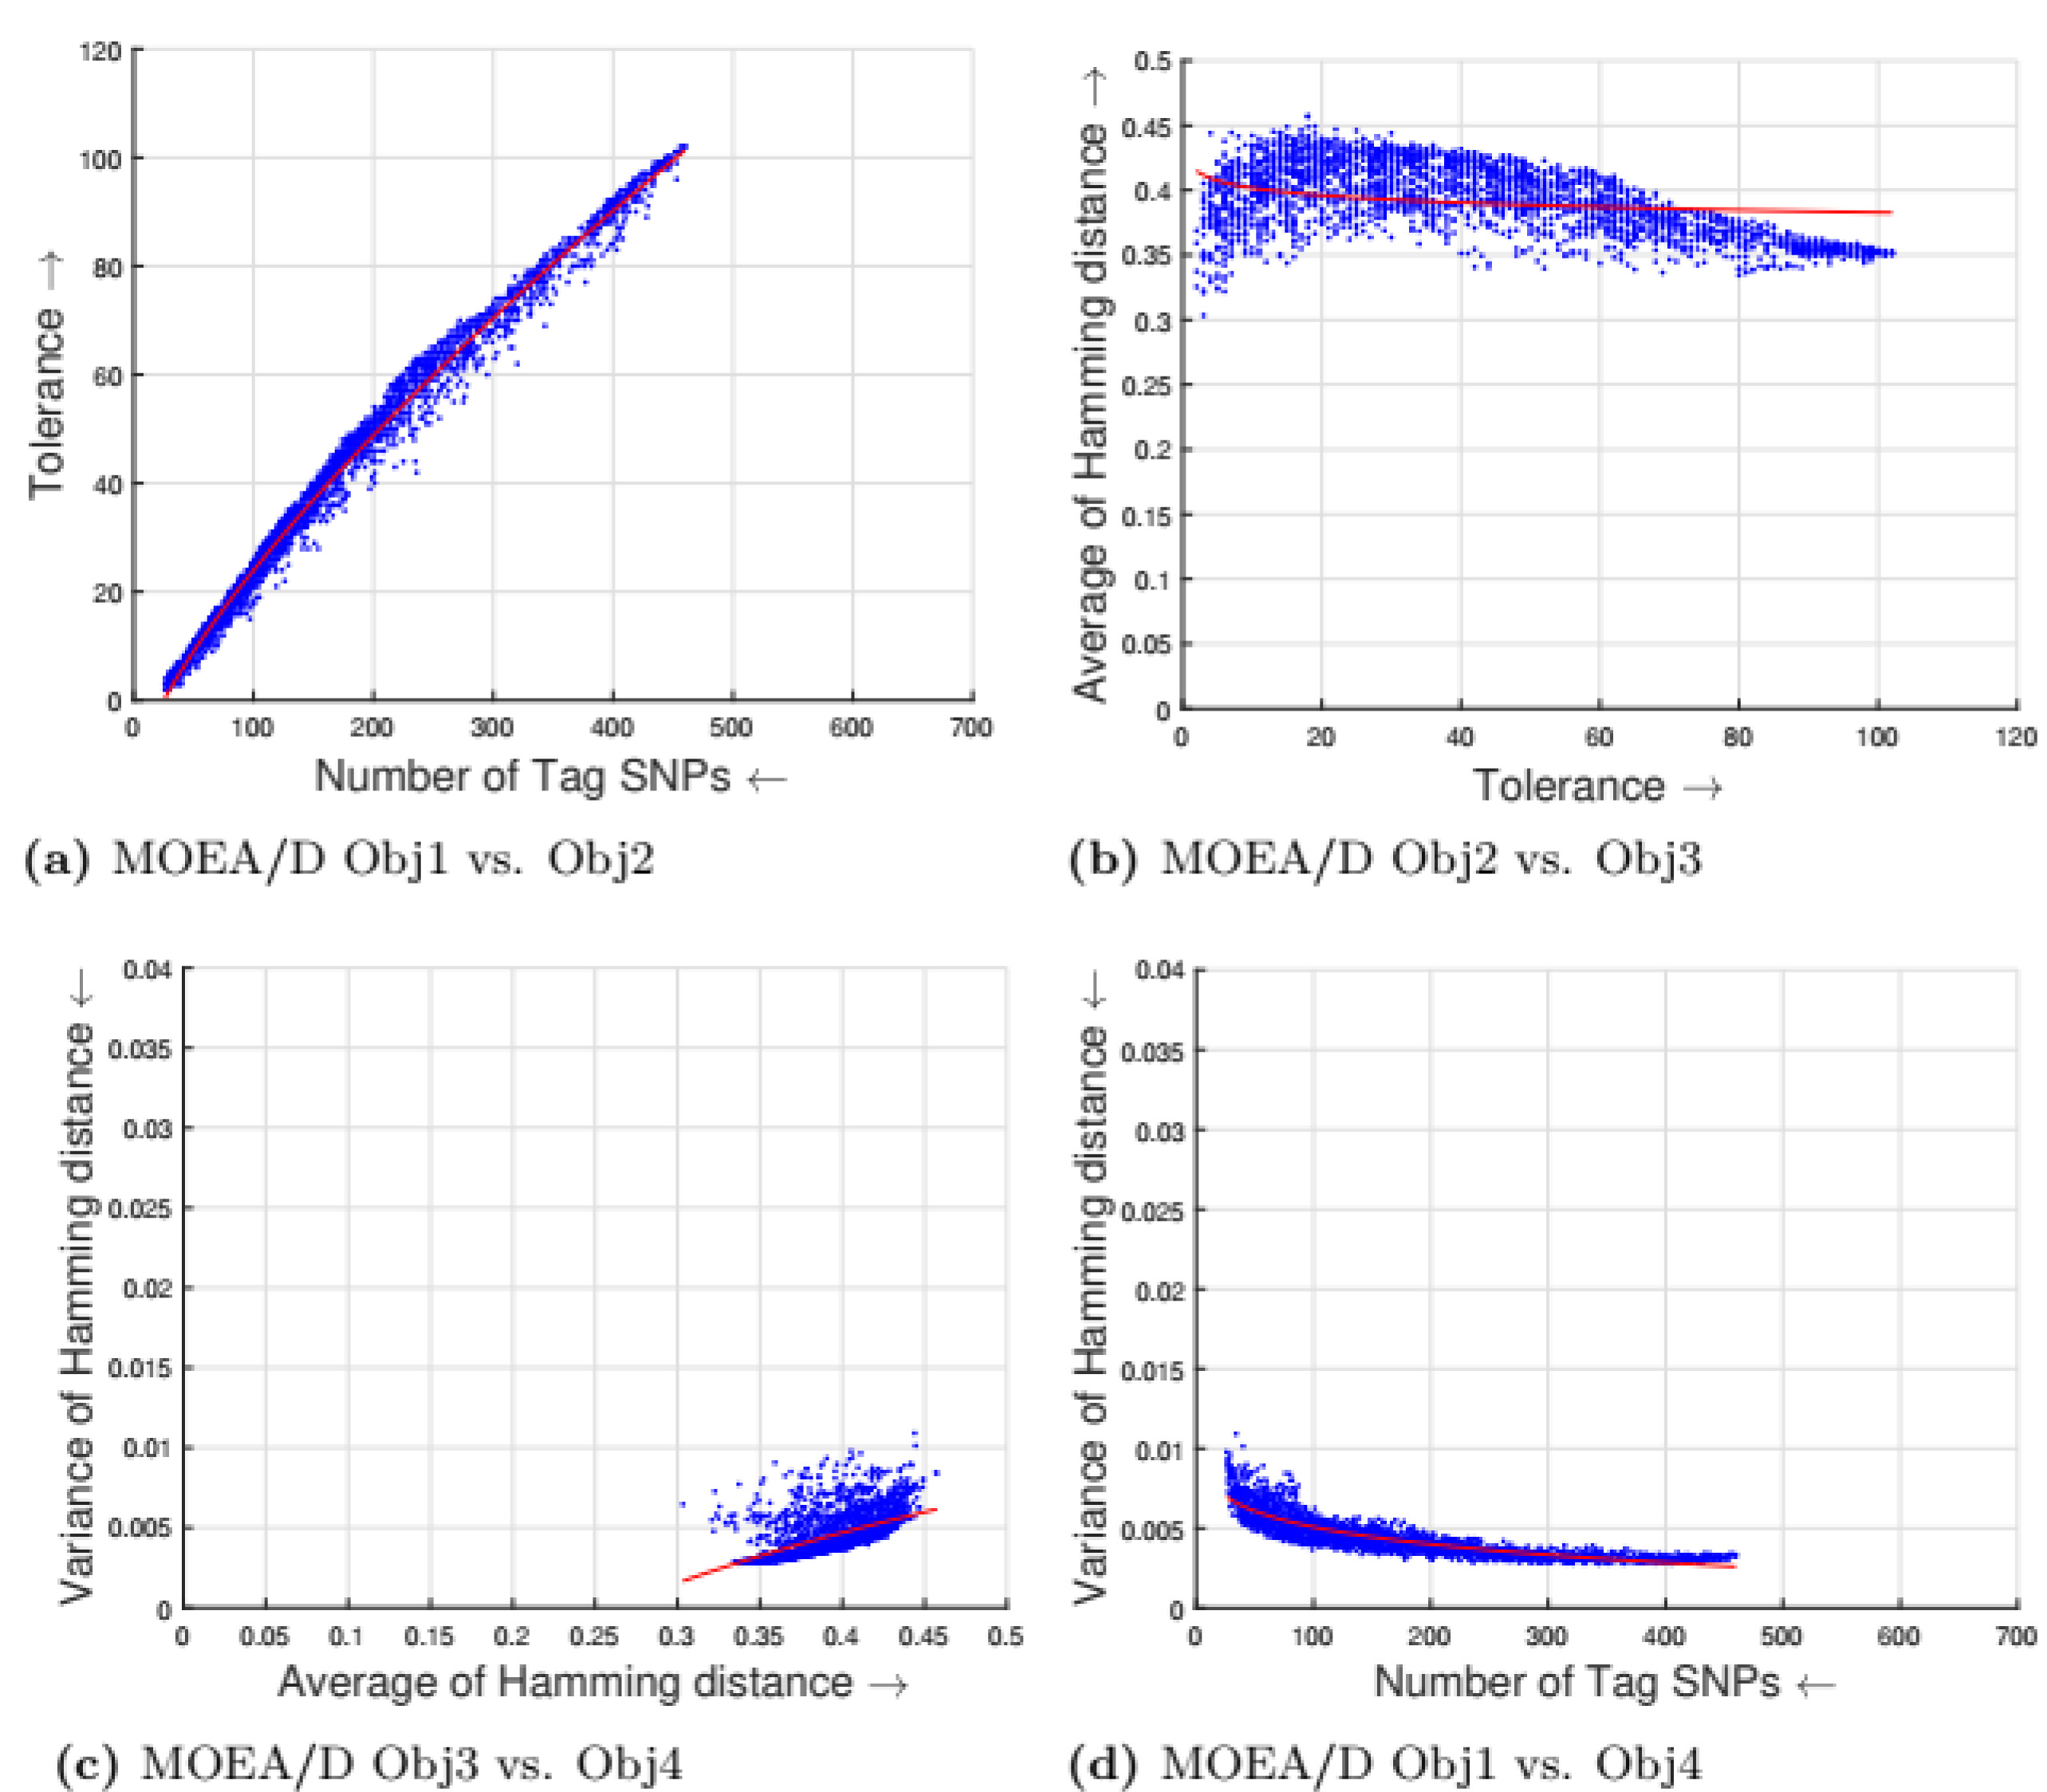
\includegraphics[width=\textwidth]{analisis_assets/moqa_2022/figures/moqa_fig_moead_random.jpeg}
        \caption{MOEA/D: Random (Moqa)}
    \end{subfigure}
    \begin{subfigure}[b]{0.32\textwidth}
        \centering
        
\includegraphics[width=\textwidth]{analisis_assets/20260425T180636/2_comparativa/1_frentes/frentes_pareto/frentes_pareto_moead_tche_random_dense_full.png}
        \caption{TCHE: Random Dense (Exp. A)}
    \end{subfigure}
    \begin{subfigure}[b]{0.32\textwidth}
        \centering
        
\includegraphics[width=\textwidth]{analisis_assets/20260425T170417/2_comparativa/1_frentes/frentes_pareto/frentes_pareto_moead_tche_random_dense_full.png}
        \caption{TCHE: Random Dense (Exp. B)}
    \end{subfigure}
    \caption{Comparativa de frentes para MOEA/D-TCHE frente al original de Moqa (Greedy y Random).}
\end{figure}

\subsubsection{MOEA/D: Análisis de la variante Weighted Sum (WS)}

\begin{figure}[H]
    \centering
    \begin{subfigure}[b]{0.32\textwidth}
        \centering
        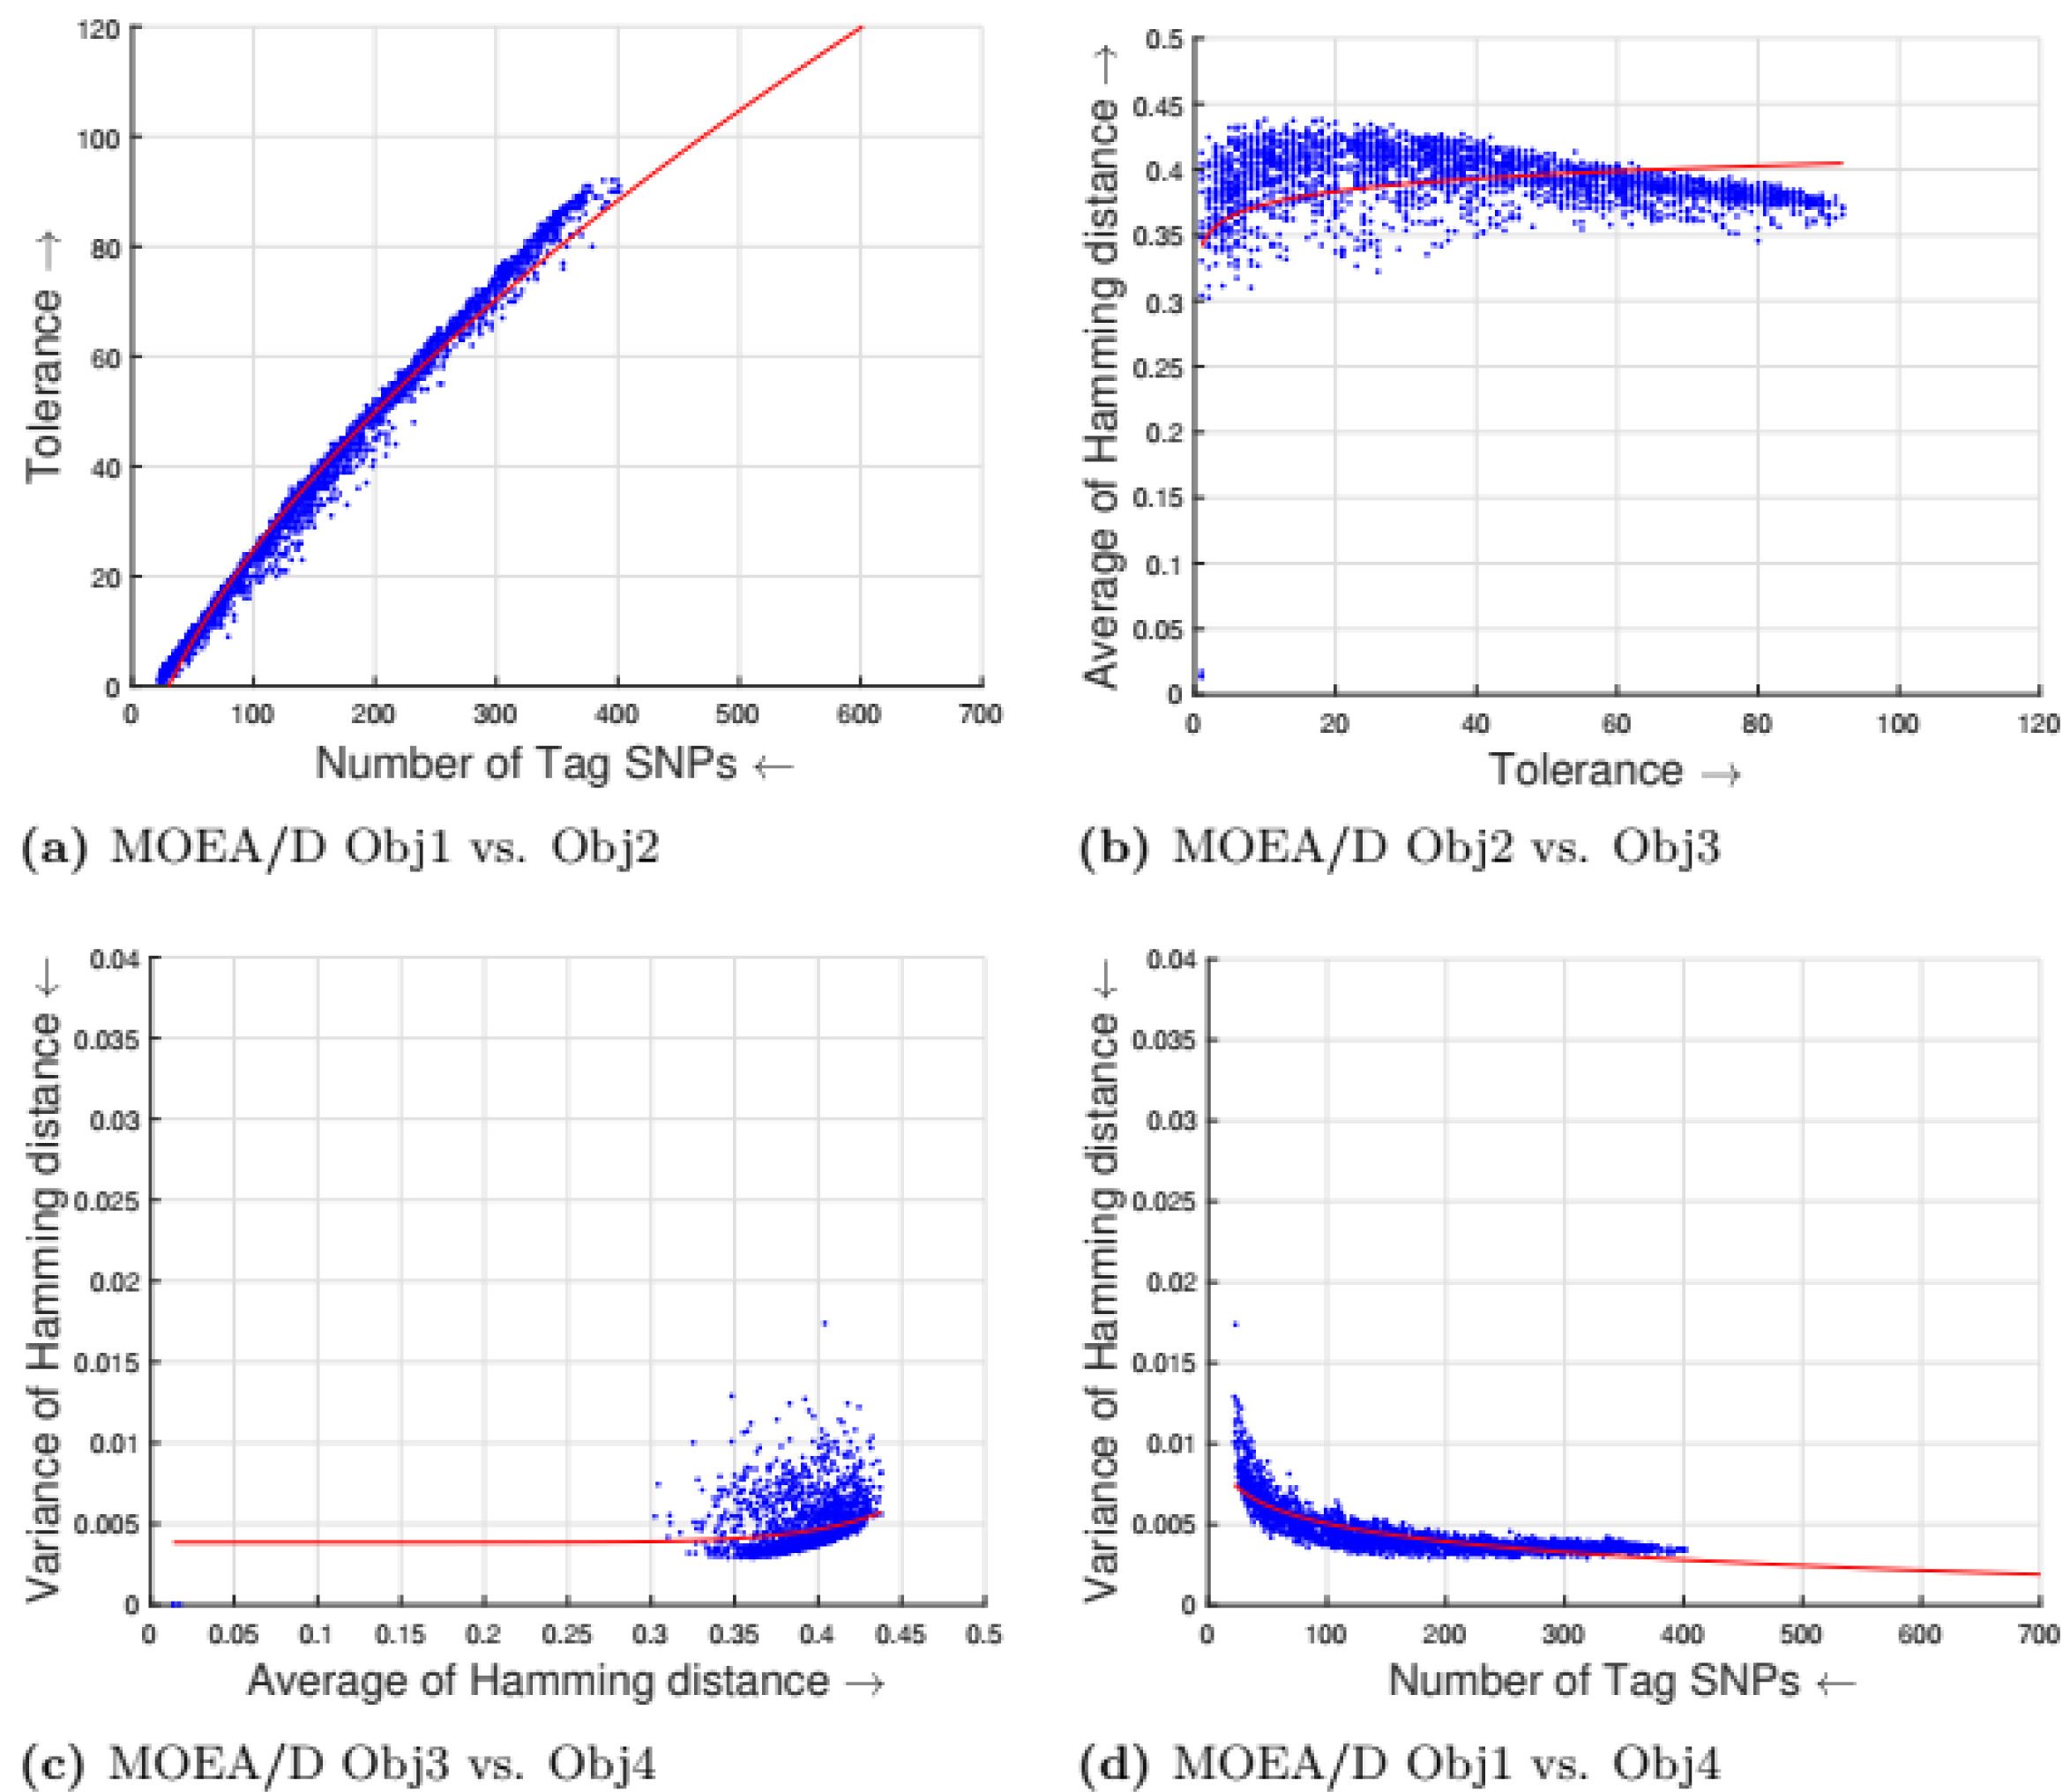
\includegraphics[width=\textwidth]{analisis_assets/moqa_2022/figures/moqa_fig_moead_greedy.jpeg}
        \caption{MOEA/D: Greedy (Moqa)}
    \end{subfigure}
    \begin{subfigure}[b]{0.32\textwidth}
        \centering
        
\includegraphics[width=\textwidth]{analisis_assets/20260425T180636/2_comparativa/1_frentes/frentes_pareto/frentes_pareto_moead_ws_greedy_hybrid_full.png}
        \caption{WS: Greedy Hybrid (Exp. A)}
    \end{subfigure}
    \begin{subfigure}[b]{0.32\textwidth}
        \centering
        
\includegraphics[width=\textwidth]{analisis_assets/20260425T170417/2_comparativa/1_frentes/frentes_pareto/frentes_pareto_moead_ws_greedy_hybrid_full.png}
        \caption{WS: Greedy Hybrid (Exp. B)}
    \end{subfigure}

    \vspace{0.3cm}

    \begin{subfigure}[b]{0.32\textwidth}
        \centering
        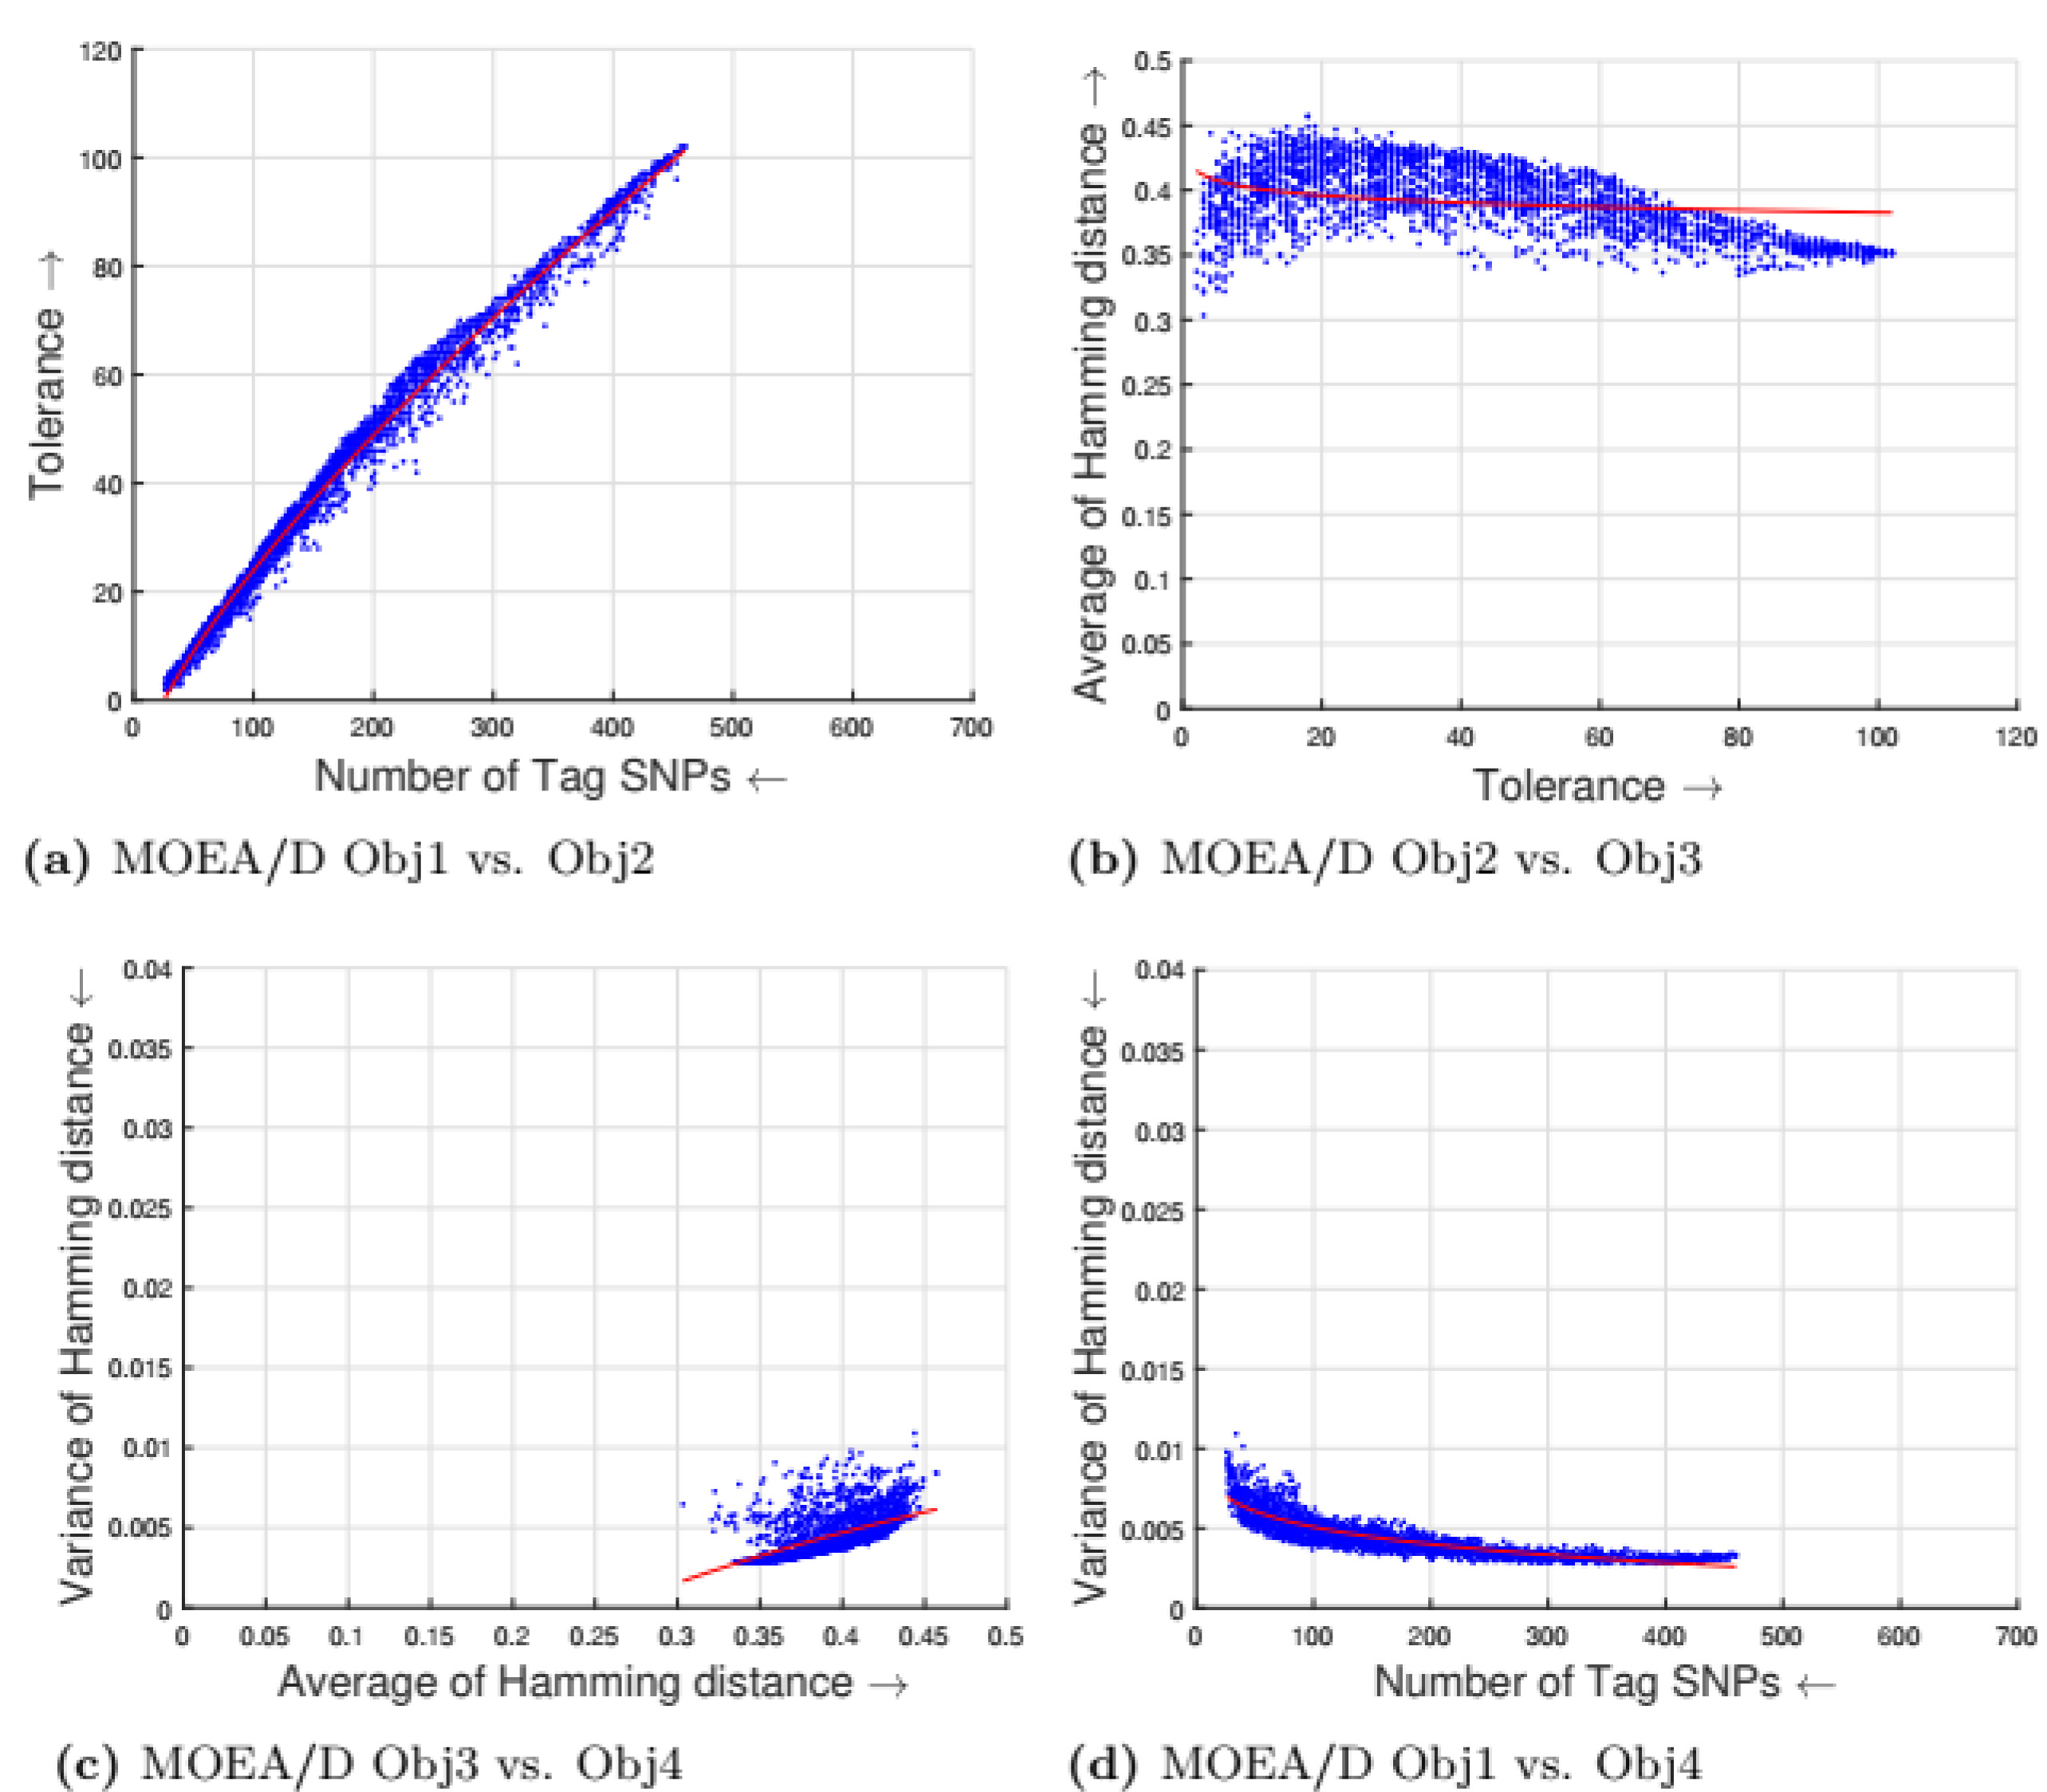
\includegraphics[width=\textwidth]{analisis_assets/moqa_2022/figures/moqa_fig_moead_random.jpeg}
        \caption{MOEA/D: Random (Moqa)}
    \end{subfigure}
    \begin{subfigure}[b]{0.32\textwidth}
        \centering
        
\includegraphics[width=\textwidth]{analisis_assets/20260425T180636/2_comparativa/1_frentes/frentes_pareto/frentes_pareto_moead_ws_random_dense_full.png}
        \caption{WS: Random Dense (Exp. A)}
    \end{subfigure}
    \begin{subfigure}[b]{0.32\textwidth}
        \centering
        
\includegraphics[width=\textwidth]{analisis_assets/20260425T170417/2_comparativa/1_frentes/frentes_pareto/frentes_pareto_moead_ws_random_dense_full.png}
        \caption{WS: Random Dense (Exp. B)}
    \end{subfigure}
    \caption{Comparativa de frentes para MOEA/D-WS frente al original de Moqa (Greedy y Random).}
\end{figure}
\subsection{Análisis Numérico y Estadístico por Métricas}
Tras la inspección visual, se procede al análisis de jerarquías de rendimiento. A continuación, se presenta el contraste de los rankings Top 8 para cada métrica, enfrentando los resultados originales de Moqa (2022) con las ejecuciones A y B de este TFG.

\subsubsection{Métrica 1: Range \texorpdfstring{($\uparrow$)}{(up)}}
\begin{table}[H]
    \centering
    \begin{minipage}[t]{0.32\textwidth}
        \centering\scriptsize\textbf{Moqa (2022)}\\
        \begin{tabular}{rl}
            \toprule
            Pos & Algo+Init \\ \midrule
            1 & MOEAD+G \\
            2 & NSGA2+G \\
            3 & NSGA3+G \\
            4 & NSGA2+R \\
            5 & SPEA2+R \\
            6 & SPEA2+G \\
            7 & NSGA3+R \\
            8 & MOEAD+R \\
            \\
            \bottomrule
        \end{tabular}
    \end{minipage}
    \hfill
    \begin{minipage}[t]{0.32\textwidth}
        \centering\scriptsize\textbf{Exp. A (neg)}\\
        \begin{tabular}{rl}
            \toprule
            Pos & Algo+Init \\ \midrule
            1 & NSGA2+GH \\
            2 & MOEAD\_W+GH \\
            3 & MOEAD\_T+GH \\
            4 & NSGA3+GH \\
            5 & SPEA2+GH \\
            6 & MOEAD\_P+GH \\
            7 & NSGA2+RD \\
            8 & NSGA2+RS \\
            \\
            \bottomrule
        \end{tabular}
    \end{minipage}
    \hfill
    \begin{minipage}[t]{0.32\textwidth}
        \centering\scriptsize\textbf{Exp. B (inv)}\\
        \begin{tabular}{rl}
            \toprule
            Pos & Algo+Init \\ \midrule
            1 & NSGA2+GH \\
            2 & NSGA2+RS \\
            3 & SPEA2+GH \\
            4 & SPEA2+RS \\
            5 & NSGA3+GH \\
            6 & MOEAD\_T+GH \\
            7 & MOEAD\_W+GH \\
            8 & NSGA3+RS \\
            \\
            \bottomrule
        \end{tabular}
    \end{minipage}
    \caption{Comparativa de Rankings: Range (Extensión del frente).}
\end{table}

\textbf{Análisis comparativo entre experimentos:}
\begin{itemize}
    \item \textbf{Similitudes:} La inicialización basada en heurísticas Greedy (G en Moqa y GH en Exp. A/B) demuestra ser la más eficaz para maximizar la extensión del frente en todos los entornos evaluados. 
    \item \textbf{Discrepancias:} Mientras que Moqa sitúa a MOEA/D como el algoritmo líder en extensión, en los experimentos A y B es NSGA-II el que ocupa sistemáticamente la primera posición del ranking. Asimismo, en el entorno recíproco (B), las inicializaciones aleatorias de baja densidad (\texttt{random\_sparse}) logran escalar hasta el Top 2, comportamiento no observado en Moqa ni en el entorno lineal (A).
\end{itemize}


\subsubsection{Métrica 2: SumMin \texorpdfstring{($\downarrow$)}{(down)}}
\begin{table}[H]
    \centering
    \begin{minipage}[t]{0.32\textwidth}
        \centering\scriptsize\textbf{Moqa (2022)}\\
        \begin{tabular}{rl}
            \toprule
            Pos & Algo+Init \\ \midrule
            1 & MOEAD+G \\
            2 & NSGA3+G \\
            3 & MOEAD+R \\
            4 & NSGA2+G \\
            5 & NSGA2+R \\
            6 & SPEA2+G \\
            7 & SPEA2+R \\
            8 & NSGA3+R \\
            \\
            \bottomrule
        \end{tabular}
    \end{minipage}
    \hfill
    \begin{minipage}[t]{0.32\textwidth}
        \centering\scriptsize\textbf{Exp. A (neg)}\\
        \begin{tabular}{rl}
            \toprule
            Pos & Algo+Init \\ \midrule
            1 & NSGA2+GH \\
            2 & MOEAD\_W+GH \\
            3 & MOEAD\_T+GH \\
            4 & NSGA3+GH \\
            5 & NSGA2+RD \\
            6 & SPEA2+GH \\
            7 & MOEAD\_P+GH \\
            8 & SPEA2+RD \\
            \\
            \bottomrule
        \end{tabular}
    \end{minipage}
    \hfill
    \begin{minipage}[t]{0.32\textwidth}
        \centering\scriptsize\textbf{Exp. B (inv)}\\
        \begin{tabular}{rl}
            \toprule
            Pos & Algo+Init \\ \midrule
            1 & NSGA2+GH \\
            2 & MOEAD\_W+GH \\
            3 & MOEAD\_T+GH \\
            4 & NSGA3+GH \\
            5 & SPEA2+GH \\
            6 & NSGA2+RS \\
            7 & SPEA2+RS \\
            8 & MOEAD\_T+RS \\
            \\
            \bottomrule
        \end{tabular}
    \end{minipage}
    \caption{Comparativa de Rankings: SumMin (Convergencia al ideal).}
\end{table}

\textbf{Análisis comparativo entre experimentos:}
\begin{itemize}
    \item \textbf{Similitudes:} Existe una coincidencia plena en la jerarquía de los experimentos A y B, donde la inicialización \texttt{greedy\_hybrid} monopoliza las primeras posiciones del ranking.
    \item \textbf{Discrepancias:} Moqa (2022) reporta a MOEA/D como el método con mejor convergencia al ideal, mientras que en este estudio NSGA-II+GH lidera de forma robusta. Se observa una discrepancia notable en la sensibilidad de NSGA-II, que en Moqa ocupa la 4ª posición pero en este estudio se consolida como el referente de convergencia.
\end{itemize}


\subsubsection{Métrica 3: MinSum \texorpdfstring{($\downarrow$)}{(down)}}
\begin{table}[H]
    \centering
    \begin{minipage}[t]{0.32\textwidth}
        \centering\scriptsize\textbf{Moqa (2022)}\\
        \begin{tabular}{rl}
            \toprule
            Pos & Algo+Init \\ \midrule
            1 & MOEAD+G \\
            2 & MOEAD+R \\
            3 & NSGA2+G \\
            4 & NSGA2+R \\
            5 & SPEA2+G \\
            6 & SPEA2+R \\
            7 & NSGA3+G \\
            8 & NSGA3+R \\
            \\
            \bottomrule
        \end{tabular}
    \end{minipage}
    \hfill
    \begin{minipage}[t]{0.32\textwidth}
        \centering\scriptsize\textbf{Exp. A (neg)}\\
        \begin{tabular}{rl}
            \toprule
            Pos & Algo+Init \\ \midrule
            1 & NSGA3+RD \\
            2 & MOEAD\_T+GH \\
            3 & SPEA2+RD \\
            4 & MOEAD\_T+RD \\
            5 & MOEAD\_P+GH \\
            6 & NSGA2+RD \\
            7 & MOEAD\_W+RD \\
            8 & NSGA3+GH \\
            \\
            \bottomrule
        \end{tabular}
    \end{minipage}
    \hfill
    \begin{minipage}[t]{0.32\textwidth}
        \centering\scriptsize\textbf{Exp. B (inv)}\\
        \begin{tabular}{rl}
            \toprule
            Pos & Algo+Init \\ \midrule
            1 & MOEAD\_W+GH \\
            2 & MOEAD\_T+GH \\
            3 & MOEAD\_T+RS \\
            4 & NSGA3+GH \\
            5 & MOEAD\_W+RS \\
            6 & NSGA3+RS \\
            7 & MOEAD\_P+RS \\
            8 & MOEAD\_P+GH \\
            \\
            \bottomrule
        \end{tabular}
    \end{minipage}
    \caption{Comparativa de Rankings: MinSum (Mejor solución individual).}
\end{table}

\textbf{Análisis comparativo entre experimentos:}
\begin{itemize}
    \item \textbf{Similitudes:} MOEA/D se confirma como el algoritmo más capacitado para encontrar la "mejor solución individual" a través de los tres experimentos, liderando los rankings de Moqa y del entorno recíproco (B).
    \item \textbf{Discrepancias:} En el entorno lineal (A), el liderazgo es asumido inesperadamente por NSGA-III vinculado a una inicialización densa (\texttt{random\_dense}), una configuración que en Moqa queda relegada a las posiciones finales (7º puesto).
\end{itemize}


\subsubsection{Métrica 4: MaxToleranceRate \texorpdfstring{($\uparrow$)}{(up)}}
\begin{table}[H]
    \centering
    \begin{minipage}[t]{0.32\textwidth}
        \centering\scriptsize\textbf{Moqa (2022)}\\
        \begin{tabular}{rl}
            \toprule
            Pos & Algo+Init \\ \midrule
            1 & NSGA3+G \\
            2 & NSGA3+R \\
            3 & MOEAD+R \\
            4 & MOEAD+G \\
            5 & NSGA2+G \\
            6 & NSGA2+R \\
            7 & SPEA2+G \\
            8 & SPEA2+R \\
            \\
            \bottomrule
        \end{tabular}
    \end{minipage}
    \hfill
    \begin{minipage}[t]{0.32\textwidth}
        \centering\scriptsize\textbf{Exp. A (neg)}\\
        \begin{tabular}{rl}
            \toprule
            Pos & Algo+Init \\ \midrule
            1 & MOEAD\_P+GH \\
            2 & NSGA3+RS \\
            3 & MOEAD\_T+GH \\
            4 & NSGA3+RD \\
            5 & SPEA2+RD \\
            6 & MOEAD\_T+RS \\
            7 & NSGA2+RD \\
            8 & MOEAD\_T+RD \\
            \\
            \bottomrule
        \end{tabular}
    \end{minipage}
    \hfill
    \begin{minipage}[t]{0.32\textwidth}
        \centering\scriptsize\textbf{Exp. B (inv)}\\
        \begin{tabular}{rl}
            \toprule
            Pos & Algo+Init \\ \midrule
            1 & MOEAD\_W+GH \\
            2 & NSGA3+RD \\
            3 & MOEAD\_T+GH \\
            4 & MOEAD\_T+RS \\
            5 & MOEAD\_W+RS \\
            6 & NSGA2+RD \\
            7 & SPEA2+RD \\
            8 & NSGA3+GH \\
            \\
            \bottomrule
        \end{tabular}
    \end{minipage}
    \caption{Comparativa de Rankings: Max Tolerance ($f_1$).}
\end{table}

\textbf{Análisis comparativo entre experimentos:}
\begin{itemize}
    \item \textbf{Similitudes:} Se observa una alta consistencia jerárquica en la que los algoritmos de muchos objetivos (\textit{many-objective}), específicamente NSGA-III y MOEA/D, dominan la captura de tolerancia en todos los entornos evaluados.
    \item \textbf{Discrepancias:} Moqa reporta un dominio exclusivo de NSGA-III en las dos primeras posiciones, mientras que en los experimentos A y B, las variantes de MOEA/D (PBI y WS) logran disputar y arrebatar el primer puesto del ranking.
\end{itemize}


\subsubsection{Métrica 5: AvgToleranceRate \texorpdfstring{($\uparrow$)}{(up)}}
\begin{table}[H]
    \centering
    \begin{minipage}[t]{0.32\textwidth}
        \centering\scriptsize\textbf{Moqa (2022)}\\
        \begin{tabular}{rl}
            \toprule
            Pos & Algo+Init \\ \midrule
            1 & MOEAD+R \\
            2 & MOEAD+G \\
            3 & NSGA3+R \\
            4 & NSGA3+G \\
            5 & NSGA2+R \\
            6 & NSGA2+G \\
            7 & SPEA2+G \\
            8 & SPEA2+R \\
            \\
            \bottomrule
        \end{tabular}
    \end{minipage}
    \hfill
    \begin{minipage}[t]{0.32\textwidth}
        \centering\scriptsize\textbf{Exp. A (neg)}\\
        \begin{tabular}{rl}
            \toprule
            Pos & Algo+Init \\ \midrule
            1 & NSGA3+RD \\
            2 & MOEAD\_P+GH \\
            3 & SPEA2+RD \\
            4 & MOEAD\_T+RD \\
            5 & NSGA2+RD \\
            6 & MOEAD\_W+RD \\
            7 & MOEAD\_P+RS \\
            8 & MOEAD\_P+RD \\
            \\
            \bottomrule
        \end{tabular}
    \end{minipage}
    \hfill
    \begin{minipage}[t]{0.32\textwidth}
        \centering\scriptsize\textbf{Exp. B (inv)}\\
        \begin{tabular}{rl}
            \toprule
            Pos & Algo+Init \\ \midrule
            1 & NSGA3+RD \\
            2 & MOEAD\_P+RS \\
            3 & MOEAD\_W+GH \\
            4 & MOEAD\_W+RD \\
            5 & MOEAD\_T+RD \\
            6 & MOEAD\_W+RS \\
            7 & NSGA2+RD \\
            8 & MOEAD\_T+RS \\
            \\
            \bottomrule
        \end{tabular}
    \end{minipage}
    \caption{Comparativa de Rankings: Avg Tolerance.}
\end{table}

\textbf{Análisis comparativo entre experimentos:}
\begin{itemize}
    \item \textbf{Similitudes:} Los algoritmos MOEA/D y NSGA-III se mantienen en el bloque superior (Top 4) en todas las ejecuciones, confirmando su estabilidad para optimizar la tasa de tolerancia promedio.
    \item \textbf{Discrepancias:} Existe una inversión en el liderazgo; mientras Moqa sitúa a MOEA/D en la cima, los experimentos A y B identifican a NSGA-III con inicialización \texttt{random\_dense} como la configuración superior.
\end{itemize}


\subsubsection{Métrica 6: Avg Hamming Distance (\texorpdfstring{$f_3$}{f3}) \texorpdfstring{($\uparrow$)}{(up)}}
\begin{table}[H]
    \centering
    \begin{minipage}[t]{0.32\textwidth}
        \centering\scriptsize\textbf{Moqa (2022)}\\
        \begin{tabular}{rl}
            \toprule
            Pos & Algo+Init \\ \midrule
            1 & SPEA2+G \\
            2 & SPEA2+R \\
            3 & NSGA2+R \\
            4 & NSGA2+G \\
            5 & NSGA3+G \\
            6 & NSGA3+R \\
            7 & MOEAD+G \\
            8 & MOEAD+R \\
            \\
            \bottomrule
        \end{tabular}
    \end{minipage}
    \hfill
    \begin{minipage}[t]{0.32\textwidth}
        \centering\scriptsize\textbf{Exp. A (neg)}\\
        \begin{tabular}{rl}
            \toprule
            Pos & Algo+Init \\ \midrule
            1 & MOEAD\_P+GP \\
            2 & MOEAD\_T+GP \\
            3 & MOEAD\_W+GP \\
            4 & NSGA3+GP \\
            5 & MOEAD\_T+RS \\
            6 & MOEAD\_W+GH \\
            7 & MOEAD\_T+GH \\
            8 & MOEAD\_W+RS \\
            \\
            \bottomrule
        \end{tabular}
    \end{minipage}
    \hfill
    \begin{minipage}[t]{0.32\textwidth}
        \centering\scriptsize\textbf{Exp. B (inv)}\\
        \begin{tabular}{rl}
            \toprule
            Pos & Algo+Init \\ \midrule
            1 & MOEAD\_P+GP \\
            2 & MOEAD\_W+GH \\
            3 & NSGA3+GP \\
            4 & MOEAD\_T+GP \\
            5 & MOEAD\_W+GP \\
            6 & MOEAD\_T+GH \\
            7 & MOEAD\_T+RS \\
            8 & MOEAD\_W+RS \\
            \\
            \bottomrule
        \end{tabular}
    \end{minipage}
    \caption{Comparativa de Rankings: Diversidad de Hamming ($f_3$).}
\end{table}

\textbf{Análisis comparativo entre experimentos:}
\begin{itemize}
    \item \textbf{Similitudes:} No se detectan similitudes jerárquicas ni numéricas significativas en esta métrica entre los estudios.
    \item \textbf{Discrepancias:} Se observa una inversión completa en la jerarquía de los algoritmos. Mientras que Moqa identifica a SPEA2 y NSGA2 como los métodos superiores, en este estudio el liderazgo es ocupado por las variantes de MOEA/D.
\end{itemize}


\subsubsection{Métrica 7: Hypervolume \texorpdfstring{($\uparrow$)}{(up)}}
\begin{table}[H]
    \centering
    \begin{minipage}[t]{0.32\textwidth}
        \centering\scriptsize\textbf{Moqa (2022)}\\
        \begin{tabular}{rl}
            \toprule
            Pos & Algo+Init \\ \midrule
            1 & Sin datos \\
            2 & Sin datos \\
            3 & Sin datos \\
            4 & Sin datos \\
            5 & Sin datos \\
            6 & Sin datos \\
            7 & Sin datos \\
            8 & Sin datos \\
            \bottomrule
        \end{tabular}
    \end{minipage}
    \hfill
    \begin{minipage}[t]{0.32\textwidth}
        \centering\scriptsize\textbf{Exp. A (neg)}\\
        \begin{tabular}{rl}
            \toprule
            Pos & Algo+Init \\ \midrule
            1 & MOEAD\_T+GH \\
            2 & NSGA2+RD \\
            3 & NSGA3+RD \\
            4 & NSGA3+GH \\
            5 & NSGA2+GH \\
            6 & SPEA2+RD \\
            7 & MOEAD\_P+GH \\
            8 & SPEA2+GH \\
            \bottomrule
        \end{tabular}
    \end{minipage}
    \hfill
    \begin{minipage}[t]{0.32\textwidth}
        \centering\scriptsize\textbf{Exp. B (inv)}\\
        \begin{tabular}{rl}
            \toprule
            Pos & Algo+Init \\ \midrule
            1 & MOEAD\_W+GH \\
            2 & MOEAD\_T+GH \\
            3 & NSGA3+GH \\
            4 & NSGA2+GH \\
            5 & SPEA2+GH \\
            6 & NSGA2+RS \\
            7 & MOEAD\_T+RS \\
            8 & NSGA3+RS \\
            \bottomrule
        \end{tabular}
    \end{minipage}
    \caption{Comparativa de Rankings: Hypervolume global.}
\end{table}

\textbf{Análisis comparativo entre experimentos:}
\begin{itemize}
    \item \textbf{Similitudes:} Ante la ausencia de datos en el estudio original, los experimentos A y B coinciden en situar a las variantes de MOEA/D (Tchebycheff y Weight Sum) como los algoritmos con mayor capacidad de cobertura del espacio objetivo. En ambos entornos, la inicialización \texttt{greedy\_hybrid} se consolida como el factor clave para entrar en el Top 5 de rendimiento.
    \item \textbf{Discrepancias:} Se observa una diferencia notable en la competitividad de las inicializaciones aleatorias. En el entorno lineal (A), la configuración \texttt{random\_dense} logra un rendimiento sobresaliente, posicionando a NSGA-II y NSGA-III en el segundo y tercer puesto del ranking respectivamente. Por el contrario, en el entorno recíproco (B), el podio es un monopolio exclusivo de \texttt{greedy\_hybrid}, mostrando una mayor dependencia de la semilla heurística para maximizar el volumen.
\end{itemize}

\subsection{Análisis del Ranking Global (Average Rank)}

Tras evaluar cada métrica de forma individual, se procede al análisis del \textit{Average Rank} global, el cual sintetiza el desempeño de cada configuración a través de las dimensiones del estudio. Este análisis se divide en dos enfoques: uno integrado que incluye todas las métricas del TFG, y otro de comparabilidad que omite el \textit{Hypervolume} para alinearse con las métricas disponibles en el estudio original.

\subsubsection{Ranking Global Integrado (7 métricas) \texorpdfstring{($\downarrow$)}{(down)}}

Esta subsección presenta el ranking global considerando la totalidad de los indicadores calculados en este TFG, incluyendo el \textit{Hypervolume} como métrica fundamental de la calidad del frente.

Cabe destacar que esta comparativa no es complemente justa, ya que el estudio original no tiene en cuenta el hypervolume como métrica de evaluación de los algoritmos. Por ello, más adelante se realizará un análisis comparativo sin incluir el hypervolume. Aún así, el hypervolume es una métrica fundamental de la calidad del frente, por lo que se incluye en el análisis global.

\begin{table}[H]
    \centering
    \begin{minipage}[t]{0.32\textwidth}
        \centering\scriptsize\textbf{Moqa (2022)}\\
        \begin{tabular}{rl}
            \toprule
            Pos & Algo+Init \\ \midrule
            1 & MOEAD+G \\
            2 & MOEAD+R \\
            3 & NSGA3+G \\
            4 & NSGA2+G \\
            5 & NSGA2+R \\
            6 & SPEA2+G \\
            7 & NSGA3+R \\
            8 & SPEA2+R \\
            \bottomrule
        \end{tabular}
    \end{minipage}
    \hfill
    \begin{minipage}[t]{0.32\textwidth}
        \centering\scriptsize\textbf{Exp. A (neg)}\\
        \begin{tabular}{rl}
            \toprule
            Pos & Algo+Init \\ \midrule
            1 & MOEAD\_T+GH \\
            2 & MOEAD\_P+GH \\
            3 & NSGA3+RD \\
            4 & NSGA2+RD \\
            5 & SPEA2+RD \\
            6 & NSGA3+GH \\
            7 & NSGA2+GH \\
            8 & MOEAD\_T+RD \\
            \bottomrule
        \end{tabular}
    \end{minipage}
    \hfill
    \begin{minipage}[t]{0.32\textwidth}
        \centering\scriptsize\textbf{Exp. B (inv)}\\
        \begin{tabular}{rl}
            \toprule
            Pos & Algo+Init \\ \midrule
            1 & MOEAD\_W+GH \\
            2 & MOEAD\_T+GH \\
            3 & MOEAD\_T+RS \\
            4 & NSGA3+GH \\
            5 & MOEAD\_W+RS \\
            6 & NSGA2+GH \\
            7 & SPEA2+GH \\
            8 & MOEAD\_P+RS \\
            \bottomrule
        \end{tabular}
    \end{minipage}
    \caption{Comparativa de Rankings Globales Integrados (7 métricas).}
\end{table}

\textbf{Análisis comparativo (Ranking Integrado):}
\begin{itemize}
    \item \textbf{Similitudes:} El ranking integrado consolida a los algoritmos basados en descomposición (MOEA/D) como los más equilibrados. En todos los casos, variantes de MOEA/D bajo inicialización dirigida (G/GH) ocupan la primera posición, demostrando robustez al promediar rendimiento en convergencia, diversidad y volumen.
    \item \textbf{Discrepancias:} En el entorno lineal (A), las inicializaciones aleatorias densas (\texttt{random\_dense}) logran escalar hasta los puestos 3, 4 y 5, mostrando una mayor competitividad que en el entorno recíproco (B), donde el podio es un monopolio de la inicialización heurística.
\end{itemize}

\subsubsection{Ranking Global de Comparabilidad (Sin Hypervolume) \texorpdfstring{($\downarrow$)}{(down)}}

Dado que el estudio original de Moqa et al. (2022) no reporta valores de \textit{Hypervolume}, esta subsección recalcula los rankings de los experimentos A y B omitiendo dicha métrica. Esto permite establecer una comparativa estrictamente basada en las 6 dimensiones compartidas: \textit{Range, SumMin, MinSum, MaxTolerance, AvgTolerance} y \textit{Hamming}.

\begin{table}[H]
    \centering
    \begin{minipage}[t]{0.32\textwidth}
        \centering\scriptsize\textbf{Moqa (2022)}\\
        \begin{tabular}{rl}
            \toprule
            Pos & Algo+Init \\ \midrule
            1 & MOEAD+G \\
            2 & MOEAD+R \\
            3 & NSGA3+G \\
            4 & NSGA2+G \\
            5 & NSGA2+R \\
            6 & SPEA2+G \\
            7 & NSGA3+R \\
            8 & SPEA2+R \\
            \bottomrule
        \end{tabular}
    \end{minipage}
    \hfill
    \begin{minipage}[t]{0.32\textwidth}
        \centering\scriptsize\textbf{Exp. A (neg)}\\
        \begin{tabular}{rl}
            \toprule
            Pos & Algo+Init \\ \midrule
            1 & MOEAD\_T+GH \\
            2 & MOEAD\_P+GH \\
            3 & NSGA3+RD \\
            4 & SPEA2+RD \\
            5 & NSGA2+RD \\
            6 & NSGA3+GH \\
            7 & MOEAD\_W+GH \\
            8 & MOEAD\_T+RD \\
            \bottomrule
        \end{tabular}
    \end{minipage}
    \hfill
    \begin{minipage}[t]{0.32\textwidth}
        \centering\scriptsize\textbf{Exp. B (inv)}\\
        \begin{tabular}{rl}
            \toprule
            Pos & Algo+Init \\ \midrule
            1 & MOEAD\_W+GH \\
            2 & MOEAD\_T+GH \\
            3 & MOEAD\_T+RS \\
            4 & NSGA3+GH \\
            5 & MOEAD\_W+RS \\
            6 & MOEAD\_P+RS \\
            7 & SPEA2+GH \\
            8 & NSGA2+GH \\
            \bottomrule
        \end{tabular}
    \end{minipage}
    \caption{Comparativa de Rankings Globales de Comparabilidad (6 métricas compartidas).}
\end{table}

\textbf{Análisis comparativo (Ranking sin Hypervolume):}
\begin{itemize}
    \item \textbf{Similitudes:} La estabilidad del ranking es el hallazgo más significativo. A pesar de retirar el indicador de volumen, el orden jerárquico de las 5 mejores configuraciones se mantiene prácticamente inalterado en ambos experimentos. Esto ratifica que el liderazgo de las variantes de MOEA/D (Tchebycheff en A y WeightSum en B) es estructural y responde a una superioridad consistente en la aproximación biológica y la convergencia de rangos, no a un sesgo de una métrica específica.
    \item \textbf{Discrepancias:} Las variaciones son mínimas y se limitan a ligeros ajustes en la mitad inferior del Top 8. En la Ejecución A, solo ocurre un intercambio de posiciones entre NSGA-II y SPEA-2 (puestos 4 y 5), mientras que en la B, la configuración \texttt{MOEAD\_P+RS} escala dos posiciones al no ser penalizada por su volumen. La alta correlación entre ambos rankings valida la robustez de la metodología y la fiabilidad de la comparativa con el paper original.
\end{itemize}

\subsection{Discusión General y Síntesis de Resultados}

Tras el análisis detallado de cada métrica y el estudio de los rankings globales, se presenta una síntesis integral que evalúe la solidez de los experimentos realizados frente al estado del arte:

\begin{itemize}
    \item \textbf{Consistencia Estructural con Moqa (2022):} A pesar de las discrepancias puntuales en el comportamiento de métricas individuales (especialmente bajo la transformación lineal de la Ejecución A), la tendencia macroscópica y la jerarquía de rendimiento de los algoritmos son consistentemente similares a las reportadas en el estudio original.
    \item \textbf{Superioridad de la Descomposición:} En las tres fuentes evaluadas (Moqa, Ejecución A y Ejecución B), MOEA/D emerge como el motor de optimización más equilibrado. Esto demuestra que la segmentación del problema en subproblemas escalares es la estrategia más robusta para el diseño de paneles de Tag SNPs, independientemente de la normalización o transformación de los objetivos aplicada.
    \item \textbf{Primacía de la Inicialización Heurística:} Se valida externamente que la calidad de la población inicial es el factor más determinante del éxito evolutivo. La brecha de rendimiento entre las configuraciones heurísticas (\texttt{greedy\_hybrid} / \texttt{greedy}) y las aleatorias es significativamente mayor que la diferencia entre los algoritmos evolutivos, tal como sugería el paper de referencia.
\end{itemize}

\section{Conclusiones generales}
El análisis comparativo integral de las ejecuciones A y B, respaldado por la validación estadística de Friedman y Nemenyi, permite extraer las siguientes conclusiones fundamentales para el TFG:

\begin{enumerate}
    \item \textbf{Impacto Crítico de la Inicialización:} La superioridad de \texttt{greedy\_hybrid} es indiscutible en ambos entornos. La combinación de una semilla heurística de alta calidad con una exploración estocástica balanceada permite a los algoritmos alcanzar frentes de Pareto más profundos y diversificados. El test de Friedman confirma que la inicialización es un factor de variabilidad de primer orden ($p < 0.05$).
    \item \textbf{Robustez del Algoritmo vs. Entorno:} Mientras que NSGA-II demuestra una robustez excepcional en el espacio lineal (A), los algoritmos basados en descomposición como MOEA/D-WS muestran una ventaja competitiva en el espacio recíproco (B). Esto sugiere que la elección del algoritmo debe estar estrechamente ligada a la transformación de objetivos aplicada.
    \item \textbf{Validez de la Validación Estadística:} La incorporación de los mapas de significancia de Nemenyi permite concluir con un nivel de confianza del 95\% qué configuraciones son genuinamente superiores, eliminando la incertidumbre asociada a la estocasticidad de las ejecuciones individuales.
    \item \textbf{Consistencia Biológica:} Independientemente de la técnica de optimización, la estrategia \texttt{random\_dense} sigue siendo la más eficaz para maximizar la representatividad biológica (Avg. Tolerance Rate), lo cual es crucial para la aplicabilidad real del panel de SNPs resultante.
    \item \textbf{Potencia Estadística y Relevancia Práctica:} Si bien algunos factores como el algoritmo no han alcanzado la significancia de forma consistente (especialmente en la Ejecución A con $p=0,0514$), se concluye que esto es una limitación de la potencia del test por el tamaño de muestra ($n=5$). No obstante, la enorme diferencia en los p-valores entre ``Algoritmo'' e ``Inicialización'' demuestra que el verdadero cuello de botella del rendimiento reside en la calidad de la población inicial y no en la arquitectura del buscador evolutivo.
\end{enumerate}

\end{document}
